\chapter{Precoding for SU-MIMO systems}
\label{chapter:su_mimo_precoding}

This chapter develops linear precoding strategies for \ac{SU}-\ac{MIMO} systems under a total transmit-power constraint.
First, we analyze the capacity in greater detail. Next, a generalized \acs{WMMSE} design framework for the joint optimization of the precoder and combiner is derived.
Finally, the performance is evaluated through Monte Carlo simulations for different system configurations.


\section{Capacity Achieving Precoding}
\label{section:capacity_achieving_precoding}
% ==========================================
%      Capacity Achieving Precoding
% ==========================================

Consider the \ac{SU}-\ac{MIMO} system model introduced in Section~\ref{subsection:su_mimo_system_model} together with the associated capacity optimization problem in \eqref{eq:capacity_su_mimo_gaussian_channel_optimization_problem}.
We first derive a more explicit expression for the channel capacity and then show that this capacity can be achieved by means of linear precoding.
Parts of this section follow a structure similar to that in Chapter 3 of~\cite{cornelis_2025}.

\subsection{SU-MIMO Capacity}
\label{subsection:su_mimo_capacity}
% ==========================
%    SU-MIMO Capacity
% ========================== 

The \ac{SVD}~\cite{svd_lecture_notes} of the channel matrix yields
\begin{equation}
\label{eq:svd_channel_matrix}
    \mathbf{H} = \mathbf{U} \boldsymbol{\Sigma} \mathbf{V}^{\mathsf{H}},
\end{equation}
where $\mathbf{U} \in \mathbb{C}^{N_R \times N_R}$ and $\mathbf{V} \in \mathbb{C}^{N_T \times N_T}$ are unitary matrices, and $\mathbf{\Sigma} \in \mathbb{R}^{N_R \times N_T}$ is a rectangular diagonal matrix which contains the singular values of $\mathbf{H}$ on its main diagonal in decreasing order.
The columns of $\mathbf{U}$ and $\mathbf{V}$ contain the left and right singular vectors of $\mathbf{H}$, respectively.

Now define the transformed variables $\tilde{\mathbf{y}} = \mathbf{U}^{\mathsf{H}} \mathbf{y}$, $\tilde{\mathbf{x}} = \mathbf{V} \mathbf{x}$, and $\tilde{\mathbf{n}} = \mathbf{U}^{\mathsf{H}} \mathbf{n}$.
Since multiplication by a unitary matrix preserves the distribution of \ac{CS} complex Gaussian noise, $\tilde{\mathbf{n}}$ has the same distribution as $\mathbf{n}$. 
Moreover, because $\mathbf{U}$ and $\mathbf{V}$ are unitary, the transformations between $(\mathbf{x},\mathbf{y})$ and $(\tilde{\mathbf{x}},\tilde{\mathbf{y}})$ are bijective. 
The original channel from~\eqref{eq:su_mimo_io} can therefore be represented equivalently as
\begin{comment}
\begin{subequations}
\label{eq:su_mimo_equivalent_io_extended}
\begin{align}
    & \mathbf{y} = \mathbf{H} \mathbf{x} + \mathbf{n} \\
    & \Leftrightarrow \quad \mathbf{y} = \mathbf{U} \mathbf{\Sigma} \mathbf{V}^{\mathsf{H}} \, \mathbf{x} + \mathbf{n} \\
    & \Leftrightarrow \quad \mathbf{U} \tilde{\mathbf{y}} = \mathbf{U} \mathbf{\Sigma} \mathbf{V}^{\mathsf{H}} \, \mathbf{V} \tilde{\mathbf{x}} + \mathbf{n} \\
    & \Leftrightarrow \quad \tilde{\mathbf{y}} = \mathbf{U}^{\mathsf{H}} \mathbf{U} \mathbf{\Sigma} \mathbf{V}^{\mathsf{H}} \mathbf{V} \, \tilde{\mathbf{x}} + \mathbf{U}^{\mathsf{H}} \mathbf{n} \\
    & \Leftrightarrow \quad \tilde{\mathbf{y}} = \mathbf{\Sigma} \tilde{\mathbf{x}} + \tilde{\mathbf{n}}.
\end{align}
\end{subequations}
\end{comment}
\begin{equation}
\label{eq:su_mimo_equivalent_io}
    \tilde{\mathbf{y}} = \mathbf{\Sigma}\tilde{\mathbf{x}} + \tilde{\mathbf{n}},
\end{equation}
which is obtained by applying the \ac{SVD} of the channel matrix and performing a change of variables. 
The channel in~\eqref{eq:su_mimo_equivalent_io} is equivalent to the original channel in the sense that the transformation preserves the mutual information between input and output. Consequently, both channels have the same capacity.

The channel matrix $\mathbf{H}$ has exactly as many non-zero singular values $\{\sigma_i\}$ as its rank, denoted as $R_H$.
Written component-wise, the equivalent channel becomes
\begin{equation}
\label{eq:su_mimo_equivalent_io_component_wise}
    \tilde{y}_i = \sigma_i \, \tilde{x}_i + \tilde{n}_i \qquad \text{for} \quad i = 1, \dots, R_H,
\end{equation}
with $\tilde{y}_i = \tilde{n}_i$ for $R_H < i \leq N_R$. 
The equivalent channel decomposes into $R_H$ independent parallel scalar Gaussian subchannels, each with their own channel gain $\sigma_i$. These subchannels and their gains are referred to as eigen subchannels and eigenmodes, respectively.
Since the components $\tilde{x}_i$ for $R_H < i \leq N_T$ have no effect on the output, they carry no information and can be set to zero.

For each eigen subchannel, the \acf{MI} is maximized by a zero-mean, \ac{CS} complex Gaussian input~\cite{telatar_1999}. Under this choice, the optimization problem~\eqref{eq:capacity_su_mimo_gaussian_channel_optimization_problem} simplifies to
\begin{equation}
\label{eq:capacity_su_mimo_gaussian_channel_optimization_problem_simplified}
\begin{aligned}
    & C = \max_{\{\mathbb{E}\left[|\tilde{x}_i|^2\right] \, \}} \; \sum_{i=1}^{R_H} \log_2\!\left(1 + \mathbb{E}\left[|\tilde{x}_i|^2\right] \, \frac{\sigma^2_i}{N_0} \right) \\
    & \text{s.t.} \quad \sum_{i=1}^{R_H} \mathbb{E}\left[|\tilde{x}_i|^2\right] \leq P_T.
\end{aligned}
\end{equation}

This maximization problem is solved using the Lagrange multiplier method (see Appendix~\ref{appendix:waterfilling}).
The variances of the channel input need to be chosen according to the waterfilling solution~\cite{gallager_1968}:
\begin{equation}
    \mathbb{E}\left[\left\|\tilde{x}_i\right\|^2\right] = \left(\mu_{\text{w}} - \frac{N_0}{\sigma^2_i}\right)_{+},
\end{equation}
where the water level $\mu_{\text{w}}$ is found iteratively to satisfy the transmit power constraint with equality.

The resulting capacity is given by
\begin{equation}
\label{eq:capacity_su_mimo_gaussian_channel}
    C = \sum_{i=1}^{R_H} \, \log_2\!\left( \max(1, \, \mu_{\text{w}} \frac{\sigma^2_i}{N_0}) \right).
\end{equation}

\subsection{Optimal Precoder Design}
\label{subsection:optimal_precoder_design}
% ==========================
%  Optimal Precoder Design
% ========================== 

In this section, we design a linear precoder and combiner that together achieve the capacity of the \ac{SU}-\ac{MIMO} channel.
We assume that the data symbol vector is \ac{CS} complex Gaussian distributed and spatially uncorrelated, and restrict ourselves to the case where the number of data streams is not fixed in advance, but can be chosen freely as part of the design.

% prove F and G achieve capacity by construction
For an arbitrary precoding matrix $\mathbf{F}$ and combining matrix $\mathbf{G}$, the data processing inequality~\cite{cover_thomas_2005} yields $I(\mathbf{x}; \mathbf{y}) \geq I(\mathbf{a}; \mathbf{z})$, where the \ac{MI} between the transmitted data symbols $\mathbf{a}$ and the decision variables $\mathbf{z}$ is given by:
\begin{subequations}
\label{eq:mi_az}
\begin{align}
    I(\mathbf{a}; \mathbf{z}) 
    &= \log_2\!\left(\det\!\left(\mathbf{I}_{N_S} + (\mathbf{G} \, \mathbf{C}_{\mathrm{n}} \, \mathbf{G}^{\mathsf{H}})^{-1} \, (\mathbf{G} \mathbf{H} \mathbf{F}) \, \mathbf{C}_{\mathrm{a}} \, (\mathbf{G} \mathbf{H} \mathbf{F})^{\mathsf{H}}\right)\right) \label{eq:mi_az_a} \\
    &= \log_2\!\left(\det\!\left(\mathbf{I}_{N_S} + \tfrac{1}{N_0}(\mathbf{G} \mathbf{G}^{\mathsf{H}})^{-1} \, (\mathbf{G} \mathbf{H} \mathbf{F}) \, (\mathbf{G} \mathbf{H} \mathbf{F})^{\mathsf{H}}\right)\right) \label{eq:mi_az_b}.
\end{align}
\end{subequations}
Expression~\eqref{eq:mi_az_a} follows directly from~\eqref{eq:mi_su_mimo_gaussian_channel} and the structural similarity between~\eqref{eq:su_mimo_io} and~\eqref{eq:su_mimo_precoding_combining_io}.
Expression~\eqref{eq:mi_az_b} then follows from~\eqref{eq:mi_az_a} upon substituting $\mathbf{C}_{\mathrm{a}} = \mathbf{I}_{N_S}$ and $\mathbf{C}_{\mathrm{n}} = N_0 \mathbf{I}_{N_R}$.

Motivated by the capacity derivation in the previous subsection, we choose the columns of $\mathbf{F}$ and the rows of $\mathbf{G}$ as the $R_H$ most dominant right and left singular vectors of $\mathbf{H}$, respectively.
These are precisely the singular vectors associated with the non-zero singular values of $\mathbf{H}$. The number of data streams is therefore chosen equal to the rank of the channel matrix.
In addition, the precoder incorporates the power allocation through a diagonal matrix $\mathbf{P}$.
More specifically, we set
\begin{equation}
\label{eq:su_mimo_optimal_precoder_and_combiner}
    \mathbf{F} = \mathbf{V}_{N_S} \, \sqrt{\mathbf{P}} \qquad \text{and} \qquad \mathbf{G} = \mathbf{U}_{N_S}^{\mathsf{H}}.
\end{equation}

It follows from~\eqref{eq:su_mimo_optimal_precoder_and_combiner} that $I(\mathbf{a}; \mathbf{z}) = I(\mathbf{x}; \mathbf{y})$ for an appropriate choice of the power allocation matrix~$\mathbf{P}$.
This result can be verified in a brute-force way by substituting the particular precoder and combiner matrices from~\eqref{eq:su_mimo_optimal_precoder_and_combiner} into~\eqref{eq:mi_az} and replacing the channel matrix by its \ac{SVD}.
\begin{comment}
\begin{subequations}
\begin{align}
    I(\mathbf{a}; \mathbf{z}) 
    &= \log_2\!\left(\det\!\left(\mathbf{I}_{N_S} + \tfrac{1}{N_0} (\mathbf{U}_{N_S}^{\mathsf{H}} \mathbf{U}_{N_S})^{-1} \, (\mathbf{U}_{N_S}^{\mathsf{H}} (\mathbf{U} \mathbf{\Sigma} \mathbf{V}^{\mathsf{H}}) \mathbf{V}_{N_S} \sqrt{\mathbf{P}}) \, (\mathbf{U}_{N_S}^{\mathsf{H}} (\mathbf{U} \mathbf{\Sigma} \mathbf{V}^{\mathsf{H}}) \mathbf{V}_{N_S} \sqrt{\mathbf{P}})^{\mathsf{H}}\right)\right) \\
    &= \log_2\!\left(\det\!\left(\mathbf{I}_{N_S} + \tfrac{1}{N_0} \mathbf{I}_{N_S} \, (\mathbf{U}_{N_S}^{\mathsf{H}} \mathbf{U} \mathbf{\Sigma} \mathbf{V}^{\mathsf{H}} \mathbf{V}_{N_S} \sqrt{\mathbf{P}}) \, (\mathbf{U}_{N_S}^{\mathsf{H}} \mathbf{U} \mathbf{\Sigma} \mathbf{V}^{\mathsf{H}} \mathbf{V}_{N_S} \sqrt{\mathbf{P}})^{\mathsf{H}}\right)\right) \\
    &= \log_2\!\left(\det\!\left(\mathbf{I}_{N_S} + \tfrac{1}{N_0} \, \left(\begin{bmatrix} \mathbf{I}_{N_S} & \mathbf{0} \end{bmatrix} \, \begin{bmatrix} \mathbf{\Sigma}_{R_H} & \mathbf{0} \\ \mathbf{0} & \mathbf{0} \end{bmatrix} \, \begin{bmatrix} \mathbf{I}_{N_S} \\ \mathbf{0} \end{bmatrix} \sqrt{\mathbf{P}}\right) \, \left(\begin{bmatrix} \mathbf{I}_{N_S} & \mathbf{0} \end{bmatrix} \, \begin{bmatrix} \mathbf{\Sigma}_{R_H} & \mathbf{0} \\ \mathbf{0} & \mathbf{0} \end{bmatrix} \, \begin{bmatrix} \mathbf{I}_{N_S} \\ \mathbf{0} \end{bmatrix} \sqrt{\mathbf{P}}\right)^{\mathsf{H}}\right)\right)  \\
    &= \log_2\!\left(\det\!\left(\mathbf{I}_{N_S} + \tfrac{1}{N_0} \, (\mathbf{\Sigma}_{N_S} \sqrt{\mathbf{P}}) \, (\mathbf{\Sigma}_{N_S} \sqrt{\mathbf{P}})^{\mathsf{H}}\right)\right) \\
    &= \log_2\!\left(\det\!\left(\mathbf{I}_{N_S} + \tfrac{1}{N_0} \, \mathbf{\Sigma}_{N_S}^2 \, \mathbf{P}\right)\right) \\
    &= \log_2\!\left( \prod_{i=1}^{N_S} \left(1 + \frac{\sigma^2_i}{N_0}\, p_i \right) \right)  \\
    &= \sum_{i=1}^{N_S} \log_2\!\left(1 + \frac{\sigma^2_i}{N_0}\, p_i \right)
\end{align}
\label{eq:mi_az_equals_mi_xy}
\end{subequations}
\end{comment}

An alternative and more elegant approach consists in substituting the particular precoder and combiner into~\eqref{eq:su_mimo_precoding_combining_io} and comparing the resulting expression with the equivalent channel given in~\eqref{eq:su_mimo_equivalent_io}.
This yields
\begin{subequations}
\label{eq:su_mimo_optimal_precoding_combining_io}
\begin{align}
    \mathbf{z} &= \mathbf{U}_{N_S}^{\mathsf{H}} \, \mathbf{U} \mathbf{\Sigma} \mathbf{V}^{\mathsf{H}} \, \mathbf{V}_{N_S} \sqrt{\mathbf{P}} \, \mathbf{a} + \mathbf{U}_{N_S}^{\mathsf{H}} \mathbf{n} \\
    %&= \begin{bmatrix} \mathbf{I}_{N_S} & \mathbf{0} \end{bmatrix} \; \begin{bmatrix} \mathbf{\Sigma}_{R_H} & \mathbf{0} \\ \mathbf{0} & \mathbf{0} \end{bmatrix} \; \begin{bmatrix} \mathbf{I}_{N_S} \\ \mathbf{0} \end{bmatrix} \; \sqrt{\mathbf{P}} \, \mathbf{a} + \tilde{\mathbf{n}} \\
    &= \mathbf{\Sigma}_{N_S} \, \sqrt{\mathbf{P}} \, \mathbf{a} + \tilde{\mathbf{n}},
\end{align}
\end{subequations}
where $\mathbf{\Sigma}_{N_S} \in \mathbb{R}^{N_S \times N_S}$ contains the $N_S = R_H$ non-zero singular values of $\mathbf{H}$ on its diagonal.
Comparing~\eqref{eq:su_mimo_optimal_precoding_combining_io} with~\eqref{eq:su_mimo_equivalent_io}, one can readily verify that $I(\mathbf{a}; \mathbf{z}) = I(\mathbf{x}; \mathbf{y})$, provided that the power allocated to each stream is set according to the waterfilling solution.
Hence, transmission with the precoder and combiner from~\eqref{eq:su_mimo_optimal_precoder_and_combiner} achieves the capacity of the \ac{SU}-\ac{MIMO} channel.
\bigskip

% interpretation optimal precoding scheme: decomposition
Denoting the $i$th element of the decision variable vector $\mathbf{z}$ by $z_i$, one can write~\eqref{eq:su_mimo_optimal_precoding_combining_io} component-wise as
\begin{equation}
\label{eq:su_mimo_optimal_precoding_combining_io_component_wise}
    z_i = \sigma_i \, \sqrt{p_i} \, a_i + \tilde{n}_i \qquad \text{for} \quad i = 1, \dots, N_S.
\end{equation}

This expression shows that the precoder and combiner in~\eqref{eq:su_mimo_optimal_precoder_and_combiner} diagonalize the \ac{SU}-\ac{MIMO} transfer matrix from~\eqref{eq:su_mimo_precoding_combining_io}.
The original \ac{SU}-\ac{MIMO} channel is decoupled into $N_S$ independent parallel scalar \ac{SISO} Gaussian subchannels with gains $\sigma_i \neq 0$, which coincides exactly with the decomposition of the equivalent channel in~\eqref{eq:su_mimo_equivalent_io_component_wise}.
A visualization of this decomposition is shown in Fig.~\ref{fig:su_mimo_channel_decomposition}.

As a result, the individual data streams become statistically independent. 
Detection therefore reduces to symbol-by-symbol processing rather than joint detection of the full decision-variable vector. 
This leads to a significant reduction in receiver complexity, especially for systems with a large number of antennas and data streams.

\begin{figure}[htb]
    \centering
    \begin{subfigure}[c]{0.45\textwidth}
        \centering
        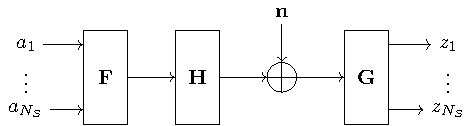
\includegraphics[width=\linewidth]
        {figures/background_material/03_su_mimo_precoding/out/channel_original.pdf}
        \caption{}
    \end{subfigure}
    \hfill
    \begin{subfigure}[c]{0.5\textwidth}
        \centering
        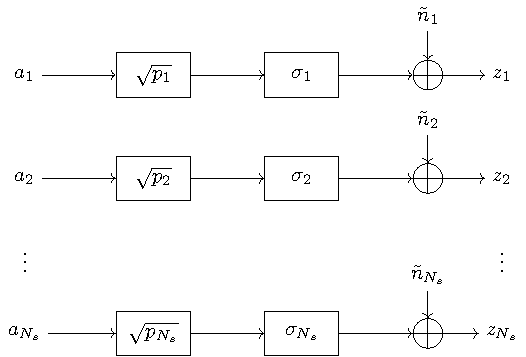
\includegraphics[width=\linewidth]
        {figures/background_material/03_su_mimo_precoding/out/channel_decomposition.pdf}
        \caption{}
    \end{subfigure}
    \caption[Decomposition of SU-MIMO channel]
    {A block diagram of the original \ac{SU}-\ac{MIMO} channel (a) and its decomposition into parallel \ac{SISO} Gaussian eigen subchannels (b) by means of the optimal precoder and combiner.}
    \label{fig:su_mimo_channel_decomposition}
\end{figure}
\bigskip

% power allocation interpretation.
No general closed-form expression exists for the optimal water level $\mu_{\mathrm{w}}$, and hence for the resulting power allocation.
Nevertheless, the optimal power allocation is fully characterized by
\begin{equation}
\label{eq:su_mimo_optimal_power_allocation}
    p_i = \left(\mu_{\mathrm{w}} - \frac{N_0}{\sigma^2_i}\right)_{+}
    \qquad \text{and} \qquad
    \sum_{i=1}^{N_S} p_i = P_T.
\end{equation}

\begin{figure}[!bt]
    \centering
    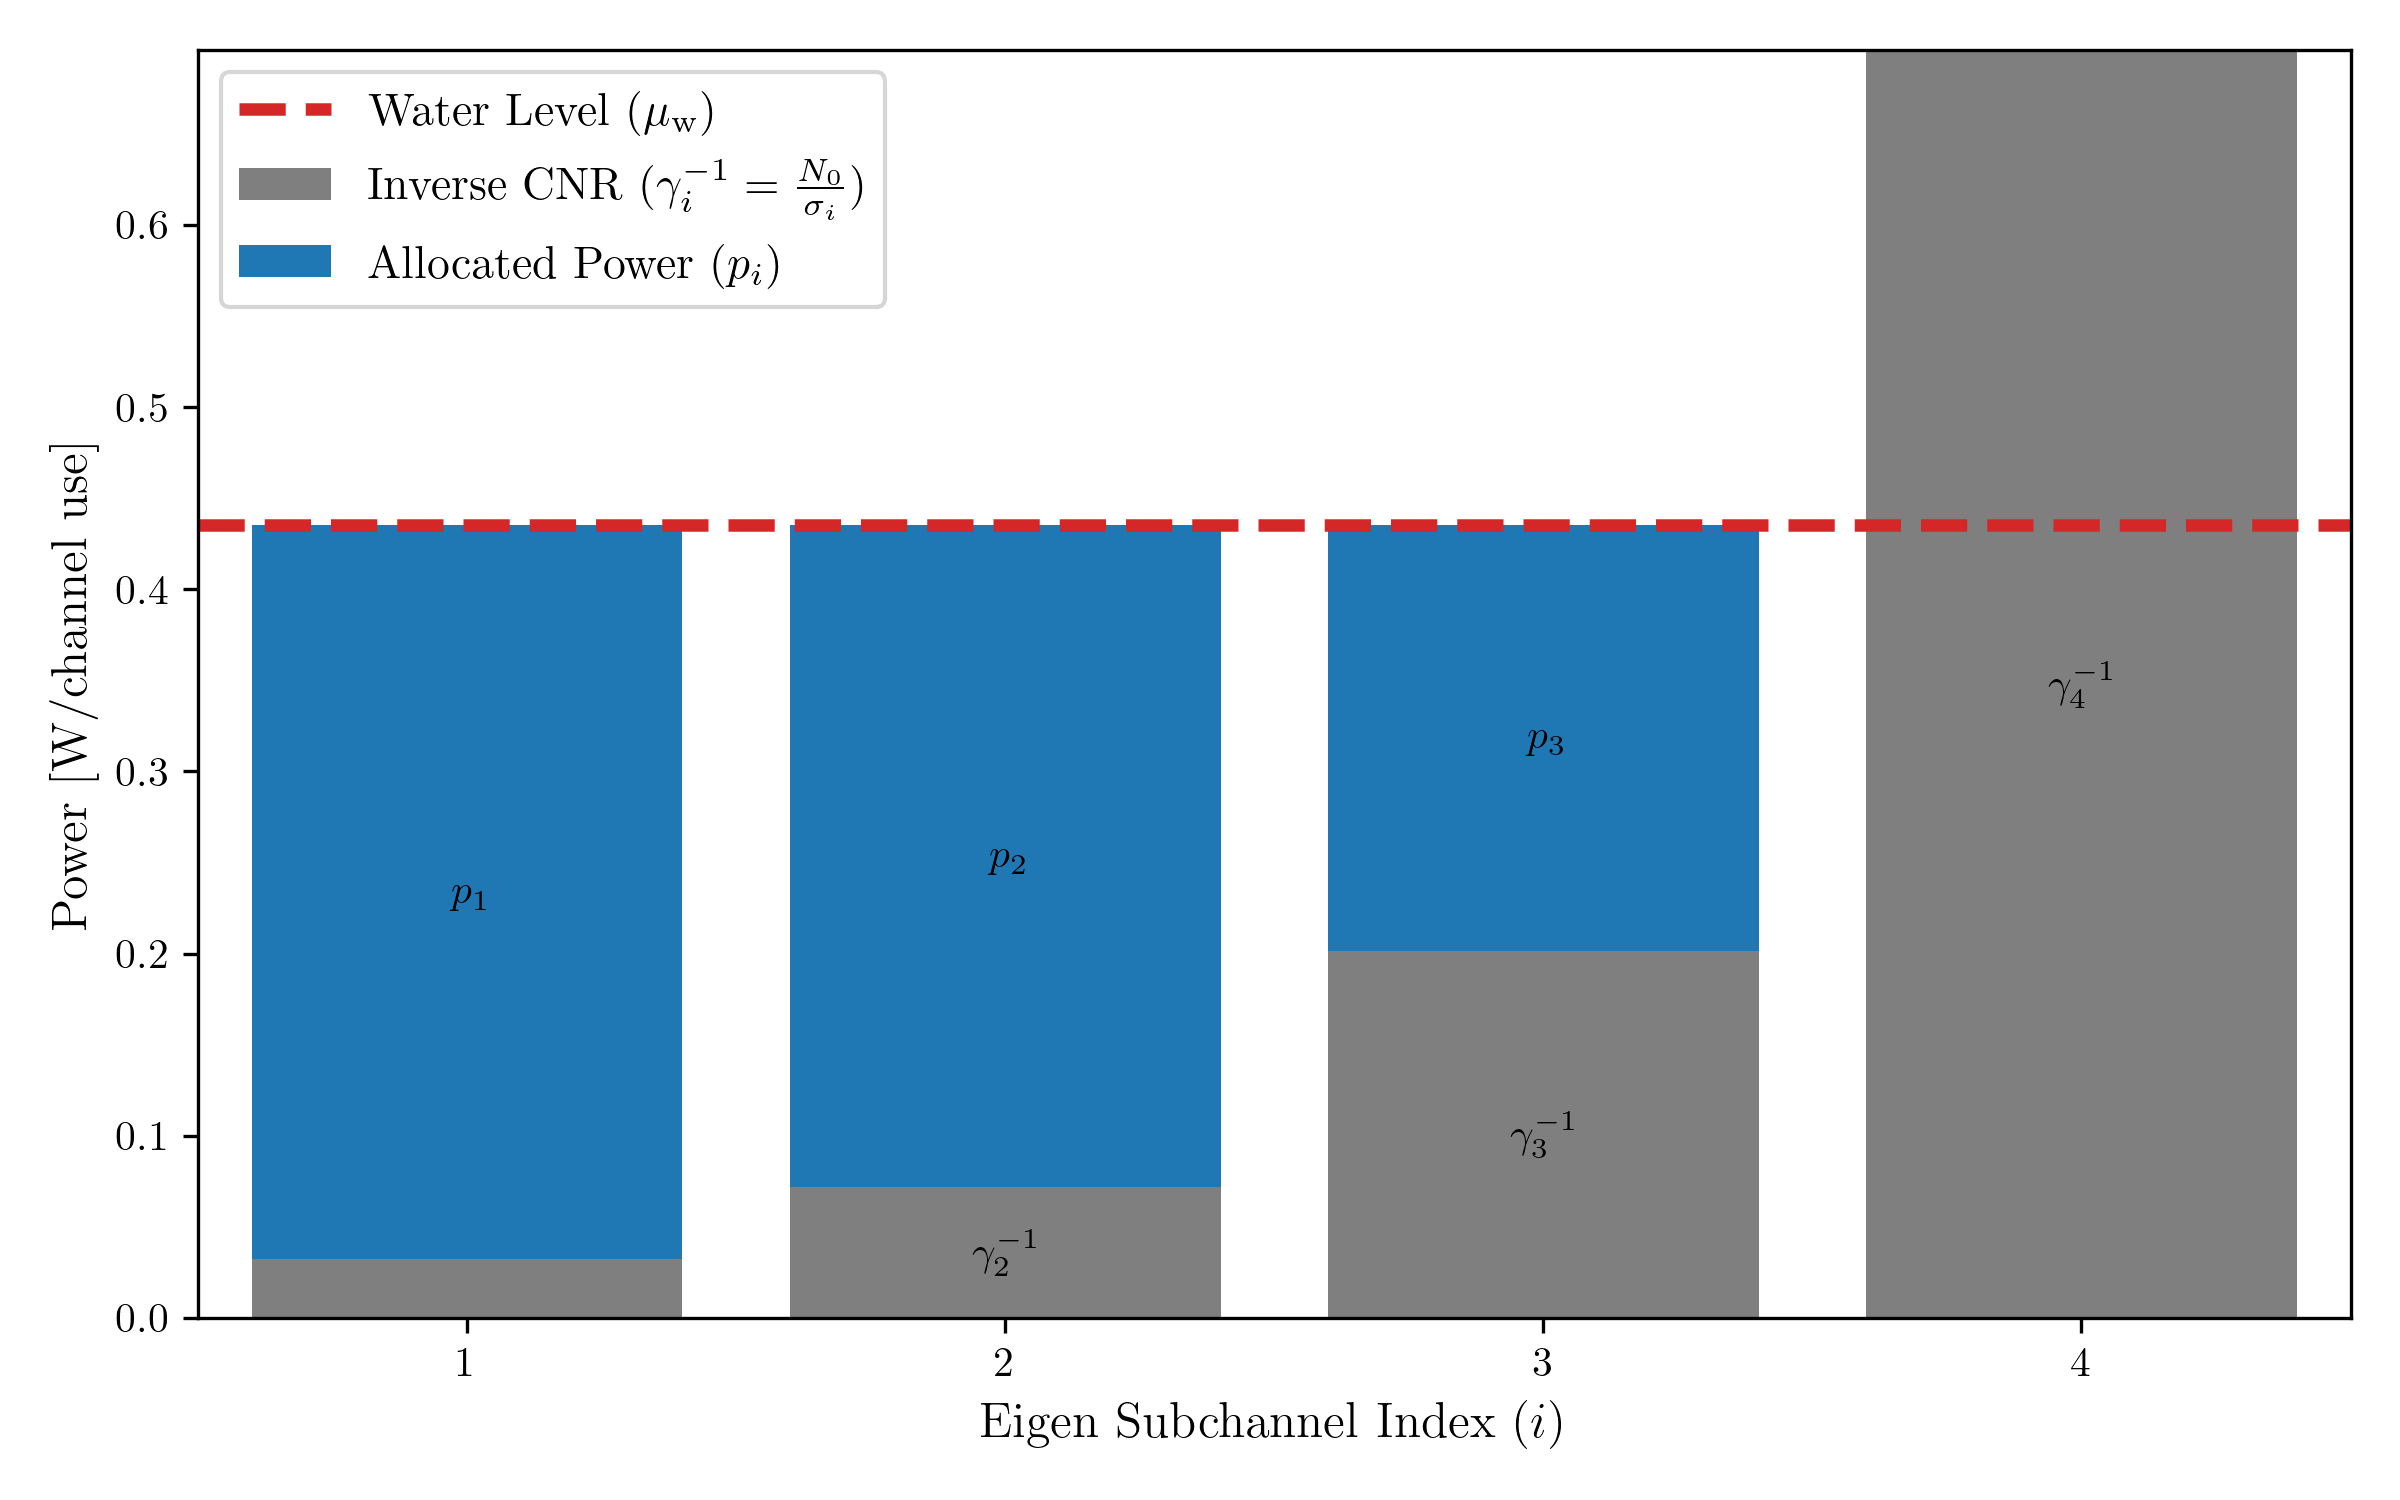
\includegraphics[width=0.6\linewidth]{figures/background_material/03_su_mimo_precoding/waterfilling/4x4__SNR_5dB.png}
    \caption[Waterfilling power allocation]
    {Optimal power allocation for a \ac{SU}-\ac{MIMO} system with 4 transmit and 4 receive antennas and a total transmit power $P_T$ of $\SI{1}{\watt}$ per channel use. The system operates at an \ac{SNR} of $5$ dB.}
    \label{fig:waterfilling_power_allocation}
\end{figure}

Since the total allocated power is a monotonically increasing function of the water level, the latter can be determined numerically by means of a bisection method.
A more efficient approach exploits the geometric interpretation of the waterfilling solution.
In the present \ac{SU}-\ac{MIMO} setting, each eigen subchannel can be represented as a container with unit width and floor level $N_0 / \sigma_i^2$, while the total transmit power is interpreted as water that is poured into these containers until a common water level is reached.
The complete procedure is summarized in Appendix~\ref{appendix_section:waterfilling_algorithm}.
The structure of the optimal power allocation is illustrated in Fig.~\ref{fig:waterfilling_power_allocation} for a \ac{SU}-\ac{MIMO} system with four transmit and four receive antennas operating at an \ac{SNR} of $5$ dB: eigen subchannels with stronger channel
conditions, i.e.\ larger gains $\sigma_i$, receive more power than weaker ones.

At extremely low \ac{SNR}, the waterfilling solution corresponds to the eigenbeamforming power allocation strategy, which concentrates all available power on the strongest eigen subchannel. As a result, only a single data stream is transmitted in this \ac{SNR} regime. This behavior is illustrated in Fig.~\ref{subfig:waterfilling_power_allocation_low_SNR}.
Conversely, at an extremely high \ac{SNR}, the optimal power allocation strategy reduces to the uniform power allocation, which distributes power equally across all eigen subchannels, as illustrated in Fig.~\ref{subfig:waterfilling_power_allocation_high_SNR}.
It is worth noting that uniform power allocation does not require knowledge of the current channel matrix, in contrast to the general waterfilling solution.

\begin{figure}[htb]
    \centering
    \begin{subfigure}[c]{0.475\textwidth}
        \centering
        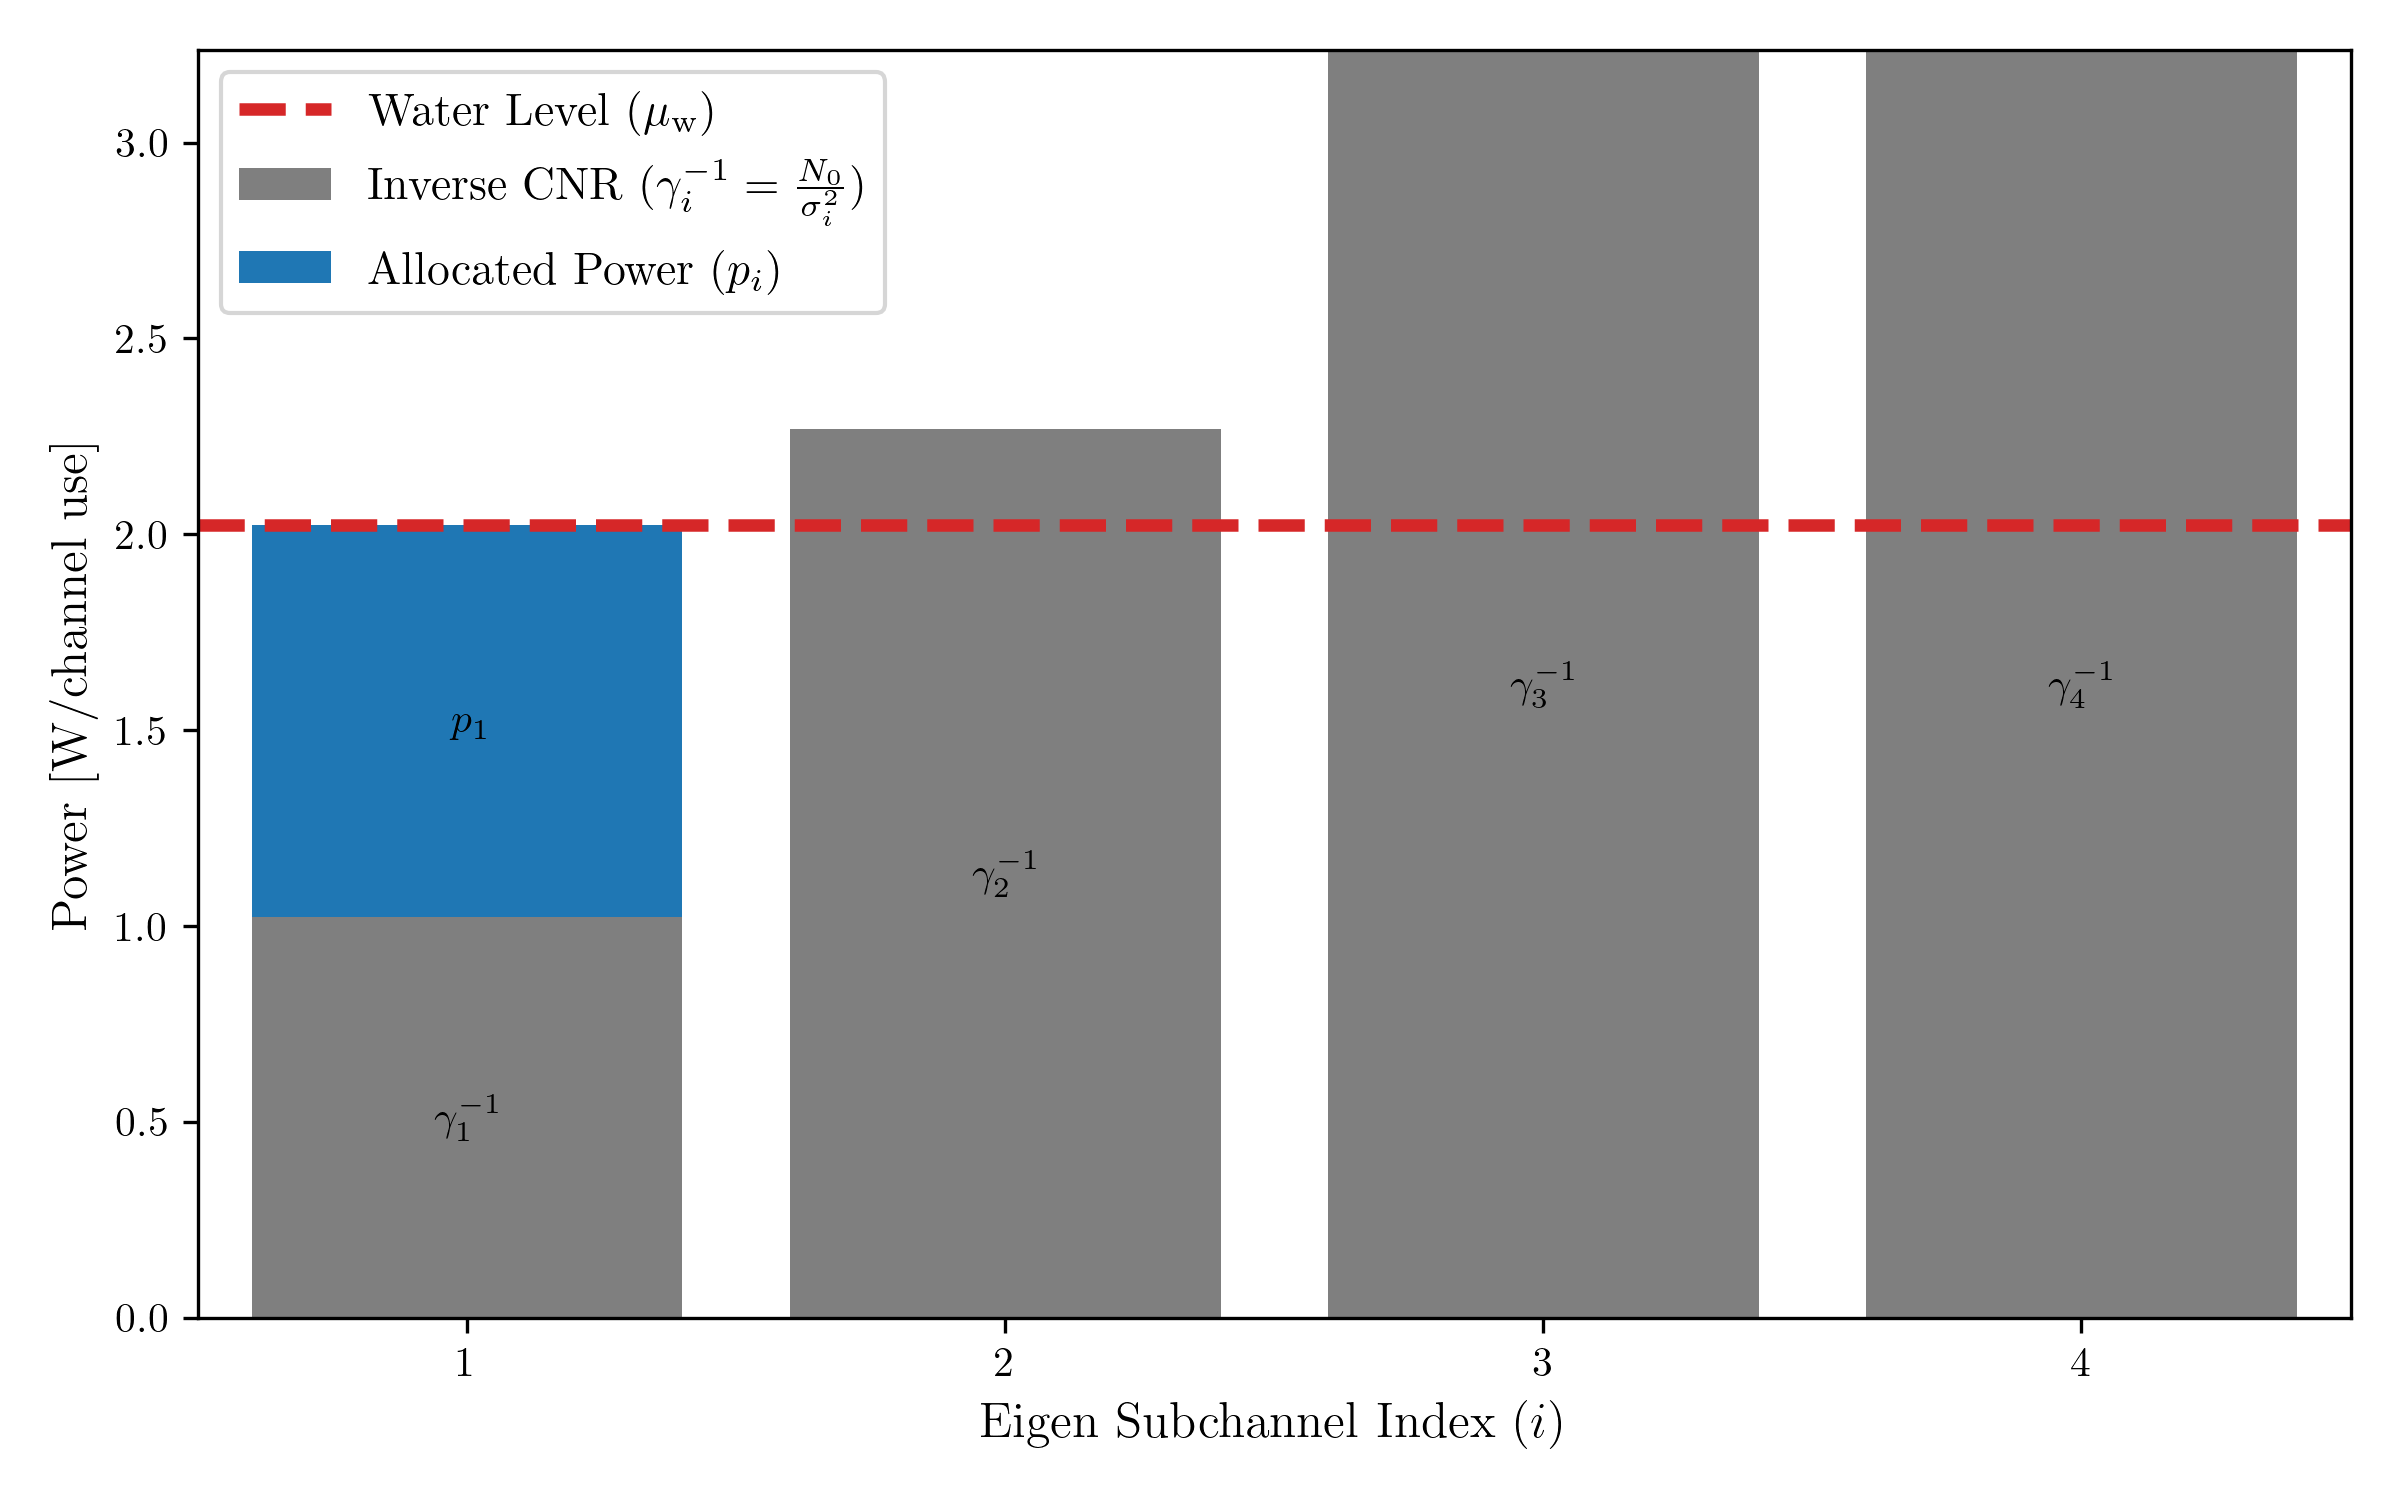
\includegraphics[width=\linewidth]
        {figures/background_material/03_su_mimo_precoding/waterfilling/4x4__SNR_-10dB.png}
        \caption{$\text{SNR} = -10 \text{ dB}$}
        \label{subfig:waterfilling_power_allocation_low_SNR}
    \end{subfigure}
    \hfill
    \begin{subfigure}[c]{0.475\textwidth}
        \centering
        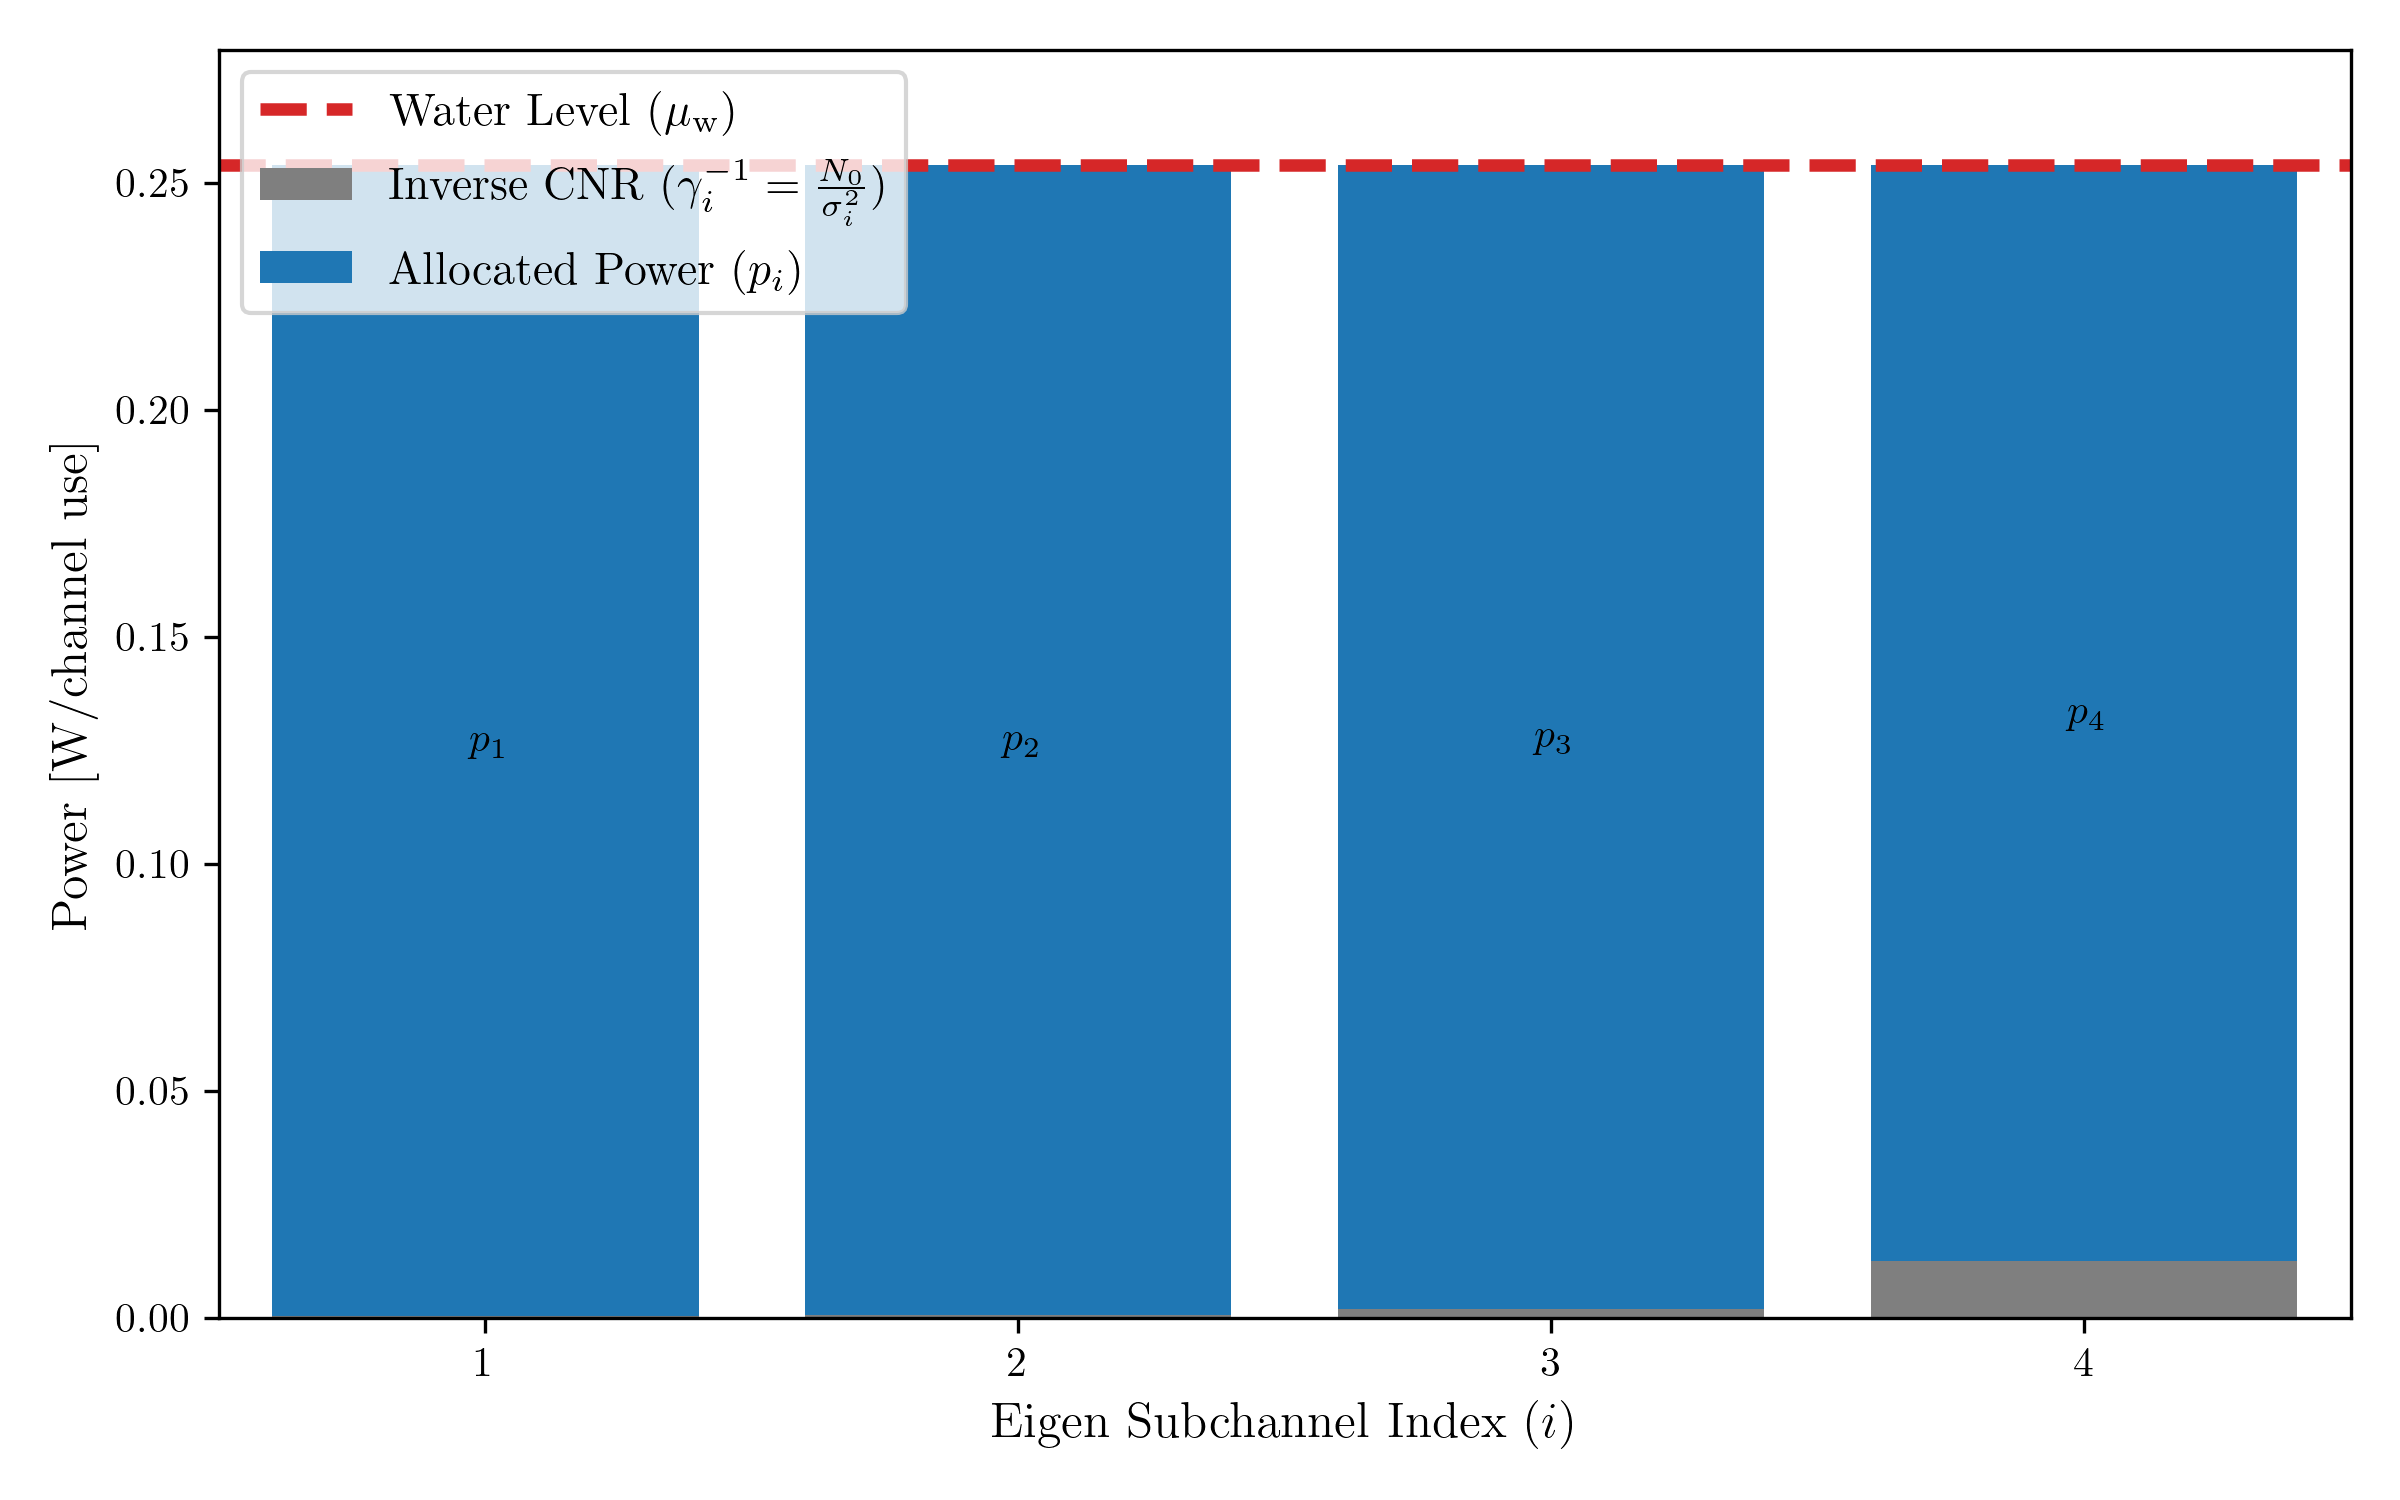
\includegraphics[width=\linewidth]
        {figures/background_material/03_su_mimo_precoding/waterfilling/4x4__SNR_25dB.png}
        \caption{$\text{SNR} = 25 \text{ dB}$}
        \label{subfig:waterfilling_power_allocation_high_SNR}
    \end{subfigure}
    \caption[Waterfilling power allocation at SNR extremes]
    {Waterfilling power allocation for a \ac{SU}-\ac{MIMO} system with 4 transmit and 4 receive antennas at different \ac{SNR} extremes. The maximum transmit power $P_T$ is $\SI{1}{\watt}$ per channel use.}

    \label{fig:waterfilling_power_allocation_SNR_extremes}
\end{figure}


\section{Joint Design for Linear Precoder and Combiner}
\label{section:joint_design_for_linear_precoder_and_combiner}
% ==========================================================
%      Joint Design for Linear Precoder and Combiner
% ==========================================================

In the previous section, a linear precoder and combiner that jointly decompose the \ac{SU}-\ac{MIMO} channel into independent parallel eigen subchannels were shown to achieve the channel capacity.
In this section, we generalize this result by adopting the minimization of a weighted sum of mean-square estimation errors as the design criterion.
It will be shown that the optimum precoder and combiner under this criterion likewise decouple the channel into parallel eigen subchannels, regardless of the specific choice of error weights.
By an appropriate selection of these weights, the framework specializes to the maximum information rate design, the \ac{QoS} design, and the unweighted \ac{MMSE} design.

\subsection{Generalized WMMSE Design}
\label{section:generalized_wmmse_design}
% ==========================
%  Generalized WMMSE Design
% ==========================

The objective is to jointly design the precoder $\mathbf{F}$ and the combiner $\mathbf{G}$ so as to minimize a weighted combination of mean-square estimation errors.
To this end, the estimation error vector $\mathbf{e} \in \mathbb{C}^{N_S}$ is defined as the difference between the transmitted data symbol vector $\mathbf{a}$ and the decision variable vector $\mathbf{z}$:
\begin{equation}
\label{eq:error_vector}
    \mathbf{e} 
    = \mathbf{a} - \mathbf{z} 
    = \mathbf{a} - (\mathbf{G}\mathbf{H}\mathbf{F}\,\mathbf{a} + \mathbf{G}\mathbf{n}).
\end{equation}

The \ac{MSE} matrix, also referred to as the error covariance matrix, is defined as
\begin{equation}
\label{eq:mse_matrix}
    \text{MSE} 
    = \mathbb{E}\!\left[\mathbf{e}\, \mathbf{e}^{\mathsf{H}}\right]
    = (\mathbf{G}\mathbf{H}\mathbf{F} - \mathbf{I}_{N_S})(\mathbf{G}\mathbf{H}\mathbf{F} - \mathbf{I}_{N_S})^{\mathsf{H}} + \mathbf{G} \mathbf{C}_{\mathrm{n}} \mathbf{G}^{\mathsf{H}}
\end{equation}
\begin{comment}
\begin{subequations}
\label{eq:mse_matrix}
\begin{align}
    \text{MSE} 
    &= \mathbb{E}\!\left[\mathbf{e}\, \mathbf{e}^{\mathsf{H}}\right] \\
    &= \mathbb{E}\!\left[(\mathbf{a} - \mathbf{G}\mathbf{H}\mathbf{F}\,\mathbf{a} - \mathbf{G}\mathbf{n}) (\mathbf{a} - \mathbf{G}\mathbf{H}\mathbf{F}\,\mathbf{a} - \mathbf{G}\mathbf{n})^{\mathsf{H}}\right] \\
    &= \mathbb{E}\!\left[(\mathbf{a} - \mathbf{G}\mathbf{H}\mathbf{F}\,\mathbf{a} - \mathbf{G}\mathbf{n}) (\mathbf{a}^{\mathsf{H}} - \mathbf{a}^{\mathsf{H}}(\mathbf{G}\mathbf{H}\mathbf{F})^{\mathsf{H}} - \mathbf{n}^{\mathsf{H}}\mathbf{G}^{\mathsf{H}})\right] \\
    &= \mathbb{E}\!\left[((\mathbf{I}_{N_S} - \mathbf{G}\mathbf{H}\mathbf{F})\,\mathbf{a} - \mathbf{G}\mathbf{n}) (\mathbf{a}^{\mathsf{H}}\,(\mathbf{I}_{N_S} - (\mathbf{G}\mathbf{H}\mathbf{F})^{\mathsf{H}}) - \mathbf{n}^{\mathsf{H}}\mathbf{G}^{\mathsf{H}})\right] \\
    &= \mathbb{E}\!\left[(\mathbf{I}_{N_S} - \mathbf{G}\mathbf{H}\mathbf{F}) \, \mathbf{a} \, \mathbf{a}^{\mathsf{H}} \, (\mathbf{I}_{N_S} - \mathbf{G}\mathbf{H}\mathbf{F})^{\mathsf{H}}\right] - \mathbb{E}\!\left[(\mathbf{I}_{N_S} - \mathbf{G}\mathbf{H}\mathbf{F}) \, \mathbf{a} \, \mathbf{n}^{\mathsf{H}}\mathbf{G}^{\mathsf{H}}\right] \notag \\
    & \quad \quad - \mathbb{E}\!\left[\mathbf{G}\mathbf{n} \, \mathbf{a}^{\mathsf{H}}\,(\mathbf{I}_{N_S} - (\mathbf{G}\mathbf{H}\mathbf{F})^{\mathsf{H}})\right] + \mathbb{E}\!\left[\mathbf{G}\mathbf{n} \, \mathbf{n}^{\mathsf{H}}\mathbf{G}^{\mathsf{H}}\right] \\
    &= (\mathbf{I}_{N_S} - \mathbf{G}\mathbf{H}\mathbf{F}) \, \mathbb{E}\!\left[\mathbf{a} \, \mathbf{a}^{\mathsf{H}}\right] \, (\mathbf{I}_{N_S} - \mathbf{G}\mathbf{H}\mathbf{F})^{\mathsf{H}} - (\mathbf{I}_{N_S} - \mathbf{G}\mathbf{H}\mathbf{F}) \, \mathbb{E}\!\left[\mathbf{a} \, \mathbf{n}^{\mathsf{H}}\right] \, \mathbf{G}^{\mathsf{H}} \notag \\
    & \quad \quad - \mathbf{G} \, \mathbb{E}\!\left[\mathbf{n} \, \mathbf{a}^{\mathsf{H}}\right] \, (\mathbf{I}_{N_S} - (\mathbf{G}\mathbf{H}\mathbf{F})^{\mathsf{H}}) + \mathbf{G} \, \mathbb{E}\!\left[\mathbf{n} \, \mathbf{n}^{\mathsf{H}}\right] \, \mathbf{G}^{\mathsf{H}}\\
    &= (\mathbf{I}_{N_S} - \mathbf{G}\mathbf{H}\mathbf{F}) \, \mathbf{I}_{N_S} \, (\mathbf{I}_{N_S} - \mathbf{G}\mathbf{H}\mathbf{F})^{\mathsf{H}} + \mathbf{G} \, \mathbf{C}_{\mathrm{n}} \, \mathbf{G}^{\mathsf{H}} \\
    &= (\mathbf{G}\mathbf{H}\mathbf{F} - \mathbf{I}_{N_S})(\mathbf{G}\mathbf{H}\mathbf{F} - \mathbf{I}_{N_S})^{\mathsf{H}} + \mathbf{G} \mathbf{C}_{\mathrm{n}} \mathbf{G}^{\mathsf{H}}
\end{align}
\end{subequations}
\end{comment}
where the last equality follows from the independence of the data symbols $\mathbf{a}$ and the noise vector $\mathbf{n}$, and the assumption that the data symbols are spatially uncorrelated and normalized.

The \ac{WMSE} is defined as
\begin{equation}
\label{eq:wmse_matrix}
    \text{WMSE} 
    = \mathbb{E}\!\left[ \left\|\mathbf{W}^{1/2}_{\mathrm{e}} \, \mathbf{e}\right\|^2 \right]
    = \mathbb{E}\!\left[ \mathrm{tr}(\mathbf{W}^{1/2}_{\mathrm{e}} \mathbf{e} \, \mathbf{e}^{\mathsf{H}} \mathbf{W}^{1/2 \, H}_{\mathrm{e}}) \right]
    = \mathrm{tr}(\mathbf{W}_{\mathrm{e}} \, \mathbb{E}\!\left[\mathbf{e} \mathbf{e}^{\mathsf{H}} \right]),
\end{equation}
where $\mathbf{W}_{\mathrm{e}}$ is a diagonal positive definite weight matrix that assigns a relative importance to the error of each data stream.

The \ac{WMMSE} optimization problem is then formulated as
\begin{equation}
\label{eq:su_mimo_WMMSE_optimization_problem}
\begin{aligned}
    & \min_{\mathbf{F}, \mathbf{G}} \; \mathrm{tr}(\mathbf{W}_{\mathrm{e}} \, \mathbb{E}\!\left[\mathbf{e} \mathbf{e}^{\mathsf{H}} \right]) \\
    & \text{s. t.} \quad \mathrm{tr}(\mathbf{F}\mathbf{F}^{\mathsf{H}}) \leq P_T.
\end{aligned}
\end{equation}

The optimization problem in~\eqref{eq:su_mimo_WMMSE_optimization_problem} can be solved using the Lagrange duality together with the \acf{KKT} conditions.
This leads to the following necessary optimality conditions~\cite{su_mimo_joint_precoder_decoder_design}:
\begin{subequations}
\begin{align}
    & \mathbf{H}\mathbf{F} = \mathbf{H}\mathbf{F} \, (\mathbf{G}\mathbf{H}\mathbf{F})^{\mathsf{H}} + \mathbf{C}_{\mathrm{n}}\mathbf{G}^{\mathsf{H}} \\
    & \mathbf{W}_{\mathrm{e}} \mathbf{G}\mathbf{H} = (\mathbf{G}\mathbf{H}\mathbf{F})^{\mathsf{H}} \, \mathbf{W}_{\mathrm{e}} \mathbf{G}\mathbf{H} + \mu \mathbf{F}^{\mathsf{H}}
\end{align}
\end{subequations}
where $\mu > 0$ is the Lagrange multiplier associated with the total transmit power constraint.

Solving these coupled matrix equations yields the optimum linear precoder and combiner.
As shown in~\cite{su_mimo_joint_precoder_decoder_design}, they admit the following closed-form expressions:
\begin{subequations}
\label{eq:solution_generalized_design}
\begin{align}
    \mathbf{F} &= \mathbf{V} \mathbf{\Phi}_{\mathrm{f}} \label{eq:solution_generalized_design_precoder}\\
    \mathbf{G} &= \mathbf{\Phi}_{\mathrm{g}} \mathbf{V}^{\mathsf{H}} \mathbf{H}^{\mathsf{H}} \mathbf{C}^{-1}_{\mathrm{n}} \label{eq:solution_generalized_design_combiner}
\end{align}
\end{subequations}
The matrices $\mathbf{\Phi}_{\mathrm{f}}, \mathbf{\Phi}_{\mathrm{g}} \in \mathbb{R}^{R_H \times R_H}$ are diagonal matrices with non-negative diagonal entries, and are given by
\begin{subequations}
\label{eq:solution_generalized_design_phi}
\begin{align}
    \mathbf{\Phi}_{\mathrm{f}} &= (\mu^{-1/2} \mathbf{\Lambda}^{-1/2} \mathbf{W}^{1/2}_{\mathrm{e}} - \mathbf{\Lambda}^{-1})^{1/2}_{+} \label{eq:solution_generalized_design_precoder_phi}\\
    \mathbf{\Phi}_{\mathrm{g}} &= (\mu^{1/2} \mathbf{\Lambda}^{-1/2} \mathbf{W}^{-1/2}_{\mathrm{e}} - \mu \mathbf{\Lambda}^{-1} \mathbf{W}^{-1}_{\mathrm{e}})^{1/2}_{+} \mathbf{\Lambda}^{1/2} \label{eq:solution_generalized_design_combiner_phi}
\end{align}
\end{subequations}
The matrices $\mathbf{V} \in \mathbb{C}^{N_T \times R_H}$ and $\mathbf{\Lambda} \in \mathbb{R}^{R_H \times R_H}$ are obtained from the \ac{EVD} of the noise-whitened Gram matrix of $\mathbf{H}$:
\begin{equation}
\label{eq:evd_generalized_design}
    \mathbf{H}^{\mathsf{H}} \mathbf{C}^{-1}_{\mathrm{n}} \mathbf{H} = \begin{bmatrix} \mathbf{V} & \bar{\mathbf{V}} \end{bmatrix} \begin{bmatrix} \mathbf{\Lambda} & \mathbf{0} \\ \mathbf{0} & \bar{\mathbf{\Lambda}} \end{bmatrix} \begin{bmatrix} \mathbf{V} & \bar{\mathbf{V}} \end{bmatrix}^{\mathsf{H}},
\end{equation}
where the columns of $\mathbf{V}$ form an orthonormal basis for the range space of $(\mathbf{H}^{\mathsf{H}} \mathbf{C}_{\mathrm{n}}^{-1} \mathbf{H})$, and the columns of $\bar{\mathbf{V}}$ span its null space.
The diagonal matrix $\mathbf{\Lambda}$ contains the $R_H$ non-zero eigenvalues arranged in descending order, whereas $\bar{\mathbf{\Lambda}}$ contains the remaining zero eigenvalues.
Note that, as in Section~\ref{subsection:optimal_precoder_design}, the number of data streams is set equal to the rank of the channel matrix, i.e.\ $N_S = R_H$. Moreover, the rank of the channel matrix is equal to the rank of $(\mathbf{H}^{\mathsf{H}} \mathbf{C}_{\mathrm{n}}^{-1} \mathbf{H})$ since $\mathbf{C}_{\mathrm{n}}^{-1}$ is positive definite and therefore does not alter the rank of the product.

Now, it only remains to show how to obtain the Lagrange multiplier that satisfies the power constraint and ensures that the bracketed matrices in both~\eqref{eq:solution_generalized_design_precoder_phi} and~\eqref{eq:solution_generalized_design_combiner_phi} are positive-definite.
Let $\mathbf{\Lambda} = \mathrm{diag}(\lambda_1, \dots, \lambda_{R_H})$ and $\mathbf{W}_{\mathrm{e}} = \mathrm{diag}(w_1, \dots, w_{R_H})$.
Suppose $k \leq R_H$ eigen subchannels are effectively used for transmission, i.e.\ they are allocated non-zero power.
From~\eqref{eq:solution_generalized_design_precoder_phi} and the total power constraint in~\eqref{eq:su_mimo_WMMSE_optimization_problem}, we have
\begin{equation}
\label{eq:power_constraint_generalized_design}
    \mathrm{tr}(\mathbf{F}\mathbf{F}^{\mathsf{H}}) = \mathrm{tr}(\mathbf{\Phi}_{\mathrm{f}}^2) = \mu^{-1/2} \sum_{i=1}^k \lambda_i^{-1/2} w^{1/2}_i - \sum_{i=1}^k \lambda_i^{-1} = P_T.
\end{equation}
Therefore, we can obtain the following expression for the Lagrange multiplier $\mu$:
\begin{equation}
\label{eq:lagrange_multiplier_generalized_design}
    \mu = \left( \frac{\sum_{i=1}^k \lambda_i^{-1/2} w^{1/2}_i}{P_T + \sum_{i=1}^k \lambda_i^{-1}} \right)^2.
\end{equation}
Let $\rho_k = \lambda_k w_k$ and let them be ordered in decreasing manner. To compute $\mathbf{\Phi}_{\mathrm{f}}$ optimally and ensure that it is positive-definite, we can compute $\mu$ according to~\eqref{eq:lagrange_multiplier_generalized_design} for each $k = 1, \dots, R_H$ iteratively, and select the largest $k$ such that $\mu \leq \rho_k$~\cite{su_mimo_joint_precoder_decoder_design}.


From~\eqref{eq:solution_generalized_design_precoder} and~\eqref{eq:solution_generalized_design_combiner}, we have:
\begin{equation}
\label{eq:diagonalization_transfer_matrix_generalized_design}
    \mathbf{T} = \mathbf{G}\mathbf{H}\mathbf{F} = \mathbf{\Phi}_{\mathrm{g}} \mathbf{\Lambda} \mathbf{\Phi}_{\mathrm{f}}.
\end{equation}
In other words, the optimum precoder and combiner diagonalize the \ac{SU}-\ac{MIMO} transfer matrix $\mathbf{T}$, and hence decouple the channel into parallel eigen subchannels, regardless of the specific choice of error weights.
This result is similar to the capacity-achieving precoder and combiner derived in Section~\ref{subsection:optimal_precoder_design}, which likewise decompose the channel matrix into parallel eigen subchannels.

By choosing the error weight matrix appropriately, the generalized \ac{WMMSE} framework can be specialized to different design criteria, such as maximum information rate, unweighted \ac{MMSE}, or prescribed quality-of-service requirements. The following subsections discuss these special cases in more detail.

\subsection{Maximum Information Rate Design}
\label{section:maximum_information_rate_design}
% =================================
%  Maximum Information Rate Design
% =================================

It was shown in Section~\ref{subsection:optimal_precoder_design} that the capacity of the \ac{SU}-\ac{MIMO} channel can be achieved by a linear precoder and combiner that diagonalize the transfer matrix and allocate power according to the waterfilling solution.
Rewriting~\eqref{eq:su_mimo_optimal_power_allocation} in matrix format and switching to the parameter notation of the generalized design yields~\cite{su_mimo_joint_precoder_decoder_design}
\begin{equation}
\label{eq:waterfilling_power_allocation_generalized_design}
    \mathbf{\Phi}_{\mathrm{f}} = (\mu^{-1/2} \mathbf{I} - \mathbf{\Lambda}^{-1})^{1/2}_{+}.
\end{equation}

The above equation is obtained by choosing the error weight matrix as $\mathbf{W}_{\mathrm{e}} = \mathbf{\Lambda}$ in~\eqref{eq:solution_generalized_design_precoder_phi}. 
It is shown in~\cite{su_mimo_joint_precoder_decoder_design} that, for this particular choice of error weights, the closed-form solutions in~\eqref{eq:solution_generalized_design_precoder} and~\eqref{eq:solution_generalized_design_combiner} yield the linear precoder and combiner that indeed maximize the information rate.
In other words, the maximum information rate design is just a special case of the generalized WMMSE design.
The choice of the error weights $\mathbf{W}_{\mathrm{e}} = \mathbf{\Lambda}$ indicates that stronger eigen subchannels support higher rates compared to the weaker ones, and hence need to be more heavily weighted in the cost function. This is consistent with the waterfilling solution, which allocates more power to stronger subchannels.

The maximum information rate design is particularly relevant in adaptive modulation systems, where more power and higher order modulation are used on eigen subchannels with higher gains to improve the total data rate.
The performance of these systems will be evaluated in Section~\ref{section:performance_evaluation}, based on simulation results for different system configurations.

\subsection{Quality of Service Design}
\label{section:quality_of_service_design}
% ===========================
%  Quality of Service Design
% ===========================
Consider an application in which different data streams carry information of heterogeneous types with different \ac{MSE} requirements for successful transmission. 
A typical example is a multimedia system in which audio and video streams are transmitted simultaneously but require different levels of reliability.
For such \acf{QoS} sensitive applications, the system must be designed to achieve prescribed \ac{MSE} levels on the individual eigen subchannels.

First, we note that the expression for the \ac{MSE} matrix simplifies upon substituting the optimum precoder and combiner from~\eqref{eq:solution_generalized_design_precoder} and~\eqref{eq:solution_generalized_design_combiner}:
\begin{equation}
\label{eq:mse_matrix_simplified}
    \text{MSE} 
    = \mathbb{E}\!\left[\mathbf{e}\, \mathbf{e}^{\mathsf{H}}\right]
    = \mathbf{W}^{-1/2}_{\mathrm{e}} \mathbf{\Lambda}^{- 1/2} \mu^{1/2}.
\end{equation}
Next, define the output \ac{SNR} matrix as
\begin{subequations}
\label{eq:snr_matrix}
\begin{align}
    \text{SNR} 
    &= (\mathbf{G}\mathbf{H}\mathbf{F})^{\mathsf{H}} \, (\mathbf{G} \mathbf{C}_{\mathrm{n}} \mathbf{G}^{\mathsf{H}})^{-1} \, (\mathbf{G}\mathbf{H}\mathbf{F}) \\
    &= \mathbf{\Phi}^2_{\mathrm{f}} \, \mathbf{\Lambda} = (\mu^{-1/2} \mathbf{\Lambda}^{1/2} \mathbf{W}^{1/2}_{\mathrm{e}} - \mathbf{I})_{+},
\end{align}
\end{subequations}
where we again used the expressions for the optimum precoder and combiner to simplify the first equality.
The relation $\text{SNR} = (\text{MSE}^{-1} - \mathbf{I})_{+}$ follows directly from these expressions, showing that the \ac{SNR} and \ac{MSE} on each subchannel are in a one-to-one inverse correspondence.
Hence, prescribing relative \acp{MSE} is equivalent to prescribing relative output \acp{SNR}.
In particular, equal \acp{SNR} across all eigen subchannels imply equal \acp{MSE}, regardless of the specific choice of error weights.

We now determine the error weight matrix $\mathbf{W}_{\mathrm{e}}$ required to realize a desired set of relative output \acp{SNR} across the eigen subchannels.
To this end, let $\mathbf{D}$ be a diagonal matrix containing the desired relative \acp{SNR}, and let $d > 0$ denote an arbitrary scaling factor.
The design requirement reduces to the following equation
\begin{equation}
\label{eq:QoS_weight_matrix_equation}
    d \, \mathbf{D} = (\mu^{-1/2} \mathbf{\Lambda}^{1/2} \mathbf{W}^{1/2}_{\mathrm{e}} - \mathbf{I})_{+},
\end{equation}
which must be solved for the weight matrix.
Assuming for simplicity that all subchannels are active, i.e.\ $\mathbf{\Phi}_{\mathrm{f}} > 0$, the corresponding solution is given by~\cite{su_mimo_joint_precoder_decoder_design}
\begin{equation}
\label{eq:QoS_weight_matrix_solution}
    \mathbf{W}^{1/2}_{\mathrm{e}} = \mu^{1/2} (d \, \mathbf{D} + \mathbf{I}) \mathbf{\Lambda}^{-1/2}
    \quad \text{with} \quad \mu^{1/2} = \frac{\mathrm{tr}(\mathbf{\Lambda}^{-1/2} \mathbf{W}^{1/2}_{\mathrm{e}})}{P_T + \mathrm{tr}(\mathbf{\Lambda}^{-1})}
    \quad \text{and} \quad d = \frac{P_T}{\mathrm{tr}(\mathbf{D} \mathbf{\Lambda}^{-1})}.
\end{equation}

As a simple example, consider an application that requires all data streams to achieve the same reliability, using a fixed rate and an identical modulation and coding scheme for all streams.
Within the present framework, this corresponds to imposing equal error rates and thus equal output \acp{SNR} on all eigen subchannels.
The latter requirement can be satisfied trivially by selecting $\mathbf{D} = \mathbf{I}$.
The resulting optimum precoder and combiner are then given by~\cite{su_mimo_joint_precoder_decoder_design}
\begin{subequations}
\label{eq:optimum_precoder_combiner_equal_errors}
\begin{align}
    \mathbf{F} &= \mathbf{V} \mathbf{\Phi}_{\mathrm{f}} 
    \quad \text{with} \quad \mathbf{\Phi}_{\mathrm{f}} = \sqrt{\frac{P_T}{\mathrm{tr}(\mathbf{\Lambda}^{-1})}} \, \mathbf{\Lambda}^{-1/2}  \\
    \mathbf{G} &= \mathbf{\Phi}_{\mathrm{g}} \mathbf{V}^{\mathsf{H}} \mathbf{H}^{\mathsf{H}} \mathbf{C}^{-1}_{\mathrm{n}} 
    \quad \text{with} \quad \mathbf{\Phi}_{\mathrm{g}} = \frac{\sqrt{P_T \, \mathrm{tr}(\mathbf{\Lambda}^{-1})}}{P_T + \mathrm{tr}(\mathbf{\Lambda}^{-1})} \, \mathbf{\Lambda}^{-1/2} 
\end{align}
\end{subequations}
This \ac{QoS} design for equal error rates allocates more power to eigen subchannels with smaller channel gains and less power to stronger eigen subchannels, such that all active subchannels achieve the same output \acp{SNR} and \acp{MSE}.
In contrast to the maximum-information-rate design, no eigen subchannels are dropped, regardless of the channel realization.
Furthermore, it can be shown that the optimum precoder and combiner transform the transfer matrix of the system into a scaled identity matrix~\cite{su_mimo_joint_precoder_decoder_design}.

\subsection{Unweighted MMSE Design}
\label{section:unweighted_mmse_design}
% ===========================
%   Unweighted MMSE Design
% ===========================
If the error weight matrix is chosen as $\mathbf{W}_{\mathrm{e}} = \mathbf{I}$, the \ac{WMMSE} problem reduces to the unweighted \acf{MMSE} design.
The closed-form solutions in~\eqref{eq:solution_generalized_design_precoder} and~\eqref{eq:solution_generalized_design_combiner} for the optimum precoder and combiner then minimize the sum of the expected squared symbol estimation errors across all eigen subchannels.
Unlike the \ac{QoS} design, this criterion does not enforce balanced performance across the individual subchannels, but improves the overall performance of the system.
In particular, substituting $\mathbf{W}_{\mathrm{e}} = \mathbf{I}$ into~\eqref{eq:mse_matrix_simplified} shows that weaker subchannels generally exhibit larger \acp{MSE}, and therefore lower output \acp{SNR}, than stronger ones.


The corresponding power allocation follows from~\eqref{eq:solution_generalized_design_precoder_phi} by setting $\mathbf{W}_{\mathrm{e}} = \mathbf{I}$, which yields
\begin{equation}
\label{eq:power_allocation_mmse_design}
    \phi_{\mathrm{f} \, i}^2 
    = \frac{1}{\sqrt{\lambda_i}} \, \left(\mu_{\mathrm{w}} - \frac{1}{\sqrt{\lambda_i}}\right)_{+}
    \qquad \text{for} \quad i = 1, \dots, R_H
\end{equation}
where $\phi_{\mathrm{f} \, i}^2$ is the $i$th element in the main diagonal of $\mathbf{\Phi}_{\mathrm{f}}$ and $\mu_{\mathrm{w}} = \mu^{-1/2}$ is a water level chosen to satisfy the total power constraint with equality.
This expression has exactly the same form as the weighted waterfilling solution derived in Appendix~\ref{appendix:waterfilling}. In particular, it is obtained from~\eqref{eq:KKT_primal_feasibility_condition1} by identifying the allocated power with $p_i = \phi_{\mathrm{f},i}^2$, the channel weight with $\alpha_i = \lambda_i^{-1/2}$, and the channel-gain-to-noise ratio with $\gamma_i = \lambda_i$.
Hence, the power allocation can be computed efficiently using Algorithm~\ref{alg:waterfilling} with these parameter choices.

As in the maximum-information-rate design, eigen subchannels whose gains fall below a threshold receive no power. 
Among the remaining active subchannels, however, the weighting factor $\alpha_i = \lambda_i^{-1/2}$ gives relatively more emphasis to weaker subchannels than in the standard sum-rate case where $\alpha_i = 1$.
This reflects the fact that the present design minimizes the total sum \ac{MSE}, rather than maximizing the information rate.


\section{Performance Evaluation}
\label{section:performance_evaluation}
% ===========================
%   Performance Evaluation
% ===========================

The preceding section derived optimal linear precoders and combiners for the \ac{SU}-\ac{MIMO} channel under several design criteria.
This section evaluates the performance of the maximum information rate design through Monte Carlo simulations.
As established in Section~\ref{section:maximum_information_rate_design}, this design is equivalent to the capacity-achieving \ac{SVD}-based precoder and combiner with waterfilling power allocation.

All simulations are conducted under the following assumptions.
The channel is modeled as an i.i.d. Rayleigh block fading channel, whose statistical model is derived in Appendix~\ref{appendix:rayleigh_channel}.
Each entry of the channel matrix $\mathbf{H}$ is drawn independently from $\mathcal{CN}(0,1)$, and the channel is held constant within a transmission block and drawn independently across blocks.
The reported performance metrics are averaged over at least $100$ independent channel realizations.
Perfect \ac{CSI} is assumed at both the \ac{TX} and the \ac{RX}, so that the precoder and combiner are computed from the exact channel matrix.

The following subsections examine the effect of different system configurations and design parameters on the system performance.
At the end of this section, analytical results are included to serve as a cross-check for the simulation curves.
All results are presented as a function of the \ac{SNR}, in terms of the total \acf{BER} and the total \acf{IBR} of the system.

\subsection{Bit Allocation Strategies}
\label{subsection:bit_allocation_strategies}
% =====================================
%    Bit Allocation Strategy
% =====================================

As a first experiment, the \ac{BER} is evaluated as a function of the \ac{SNR} for a $2 \times 2$ \ac{SU}-\ac{MIMO} system using three modulation schemes: \ac{QAM}, \ac{PSK}, and \ac{PAM}, each carrying the same number of bits per symbol.
Figure~\ref{fig:impact_constellation_2x2_fixed_ba_ber_vs_snr} shows the results under a fixed bit allocation, where the same modulation order is applied on all eigen subchannels across the entire \ac{SNR} range.
As expected, the \ac{BER} decreases monotonically with increasing \ac{SNR} for all three constellations.
The \ac{BER} curve falls most steeply for \ac{QAM}, followed by \ac{PSK} and then \ac{PAM}, confirming that \ac{QAM} reaches any given target \ac{BER} at a strictly lower \ac{SNR} than the other two schemes at equal spectral efficiency.
\ac{QAM} is therefore adopted as the modulation scheme throughout this dissertation, unless otherwise stated.
The number of bits per symbol is always chosen to be even, so that the \ac{QAM} constellation forms a regular square grid.

\begin{figure}[htb]
    \centering
    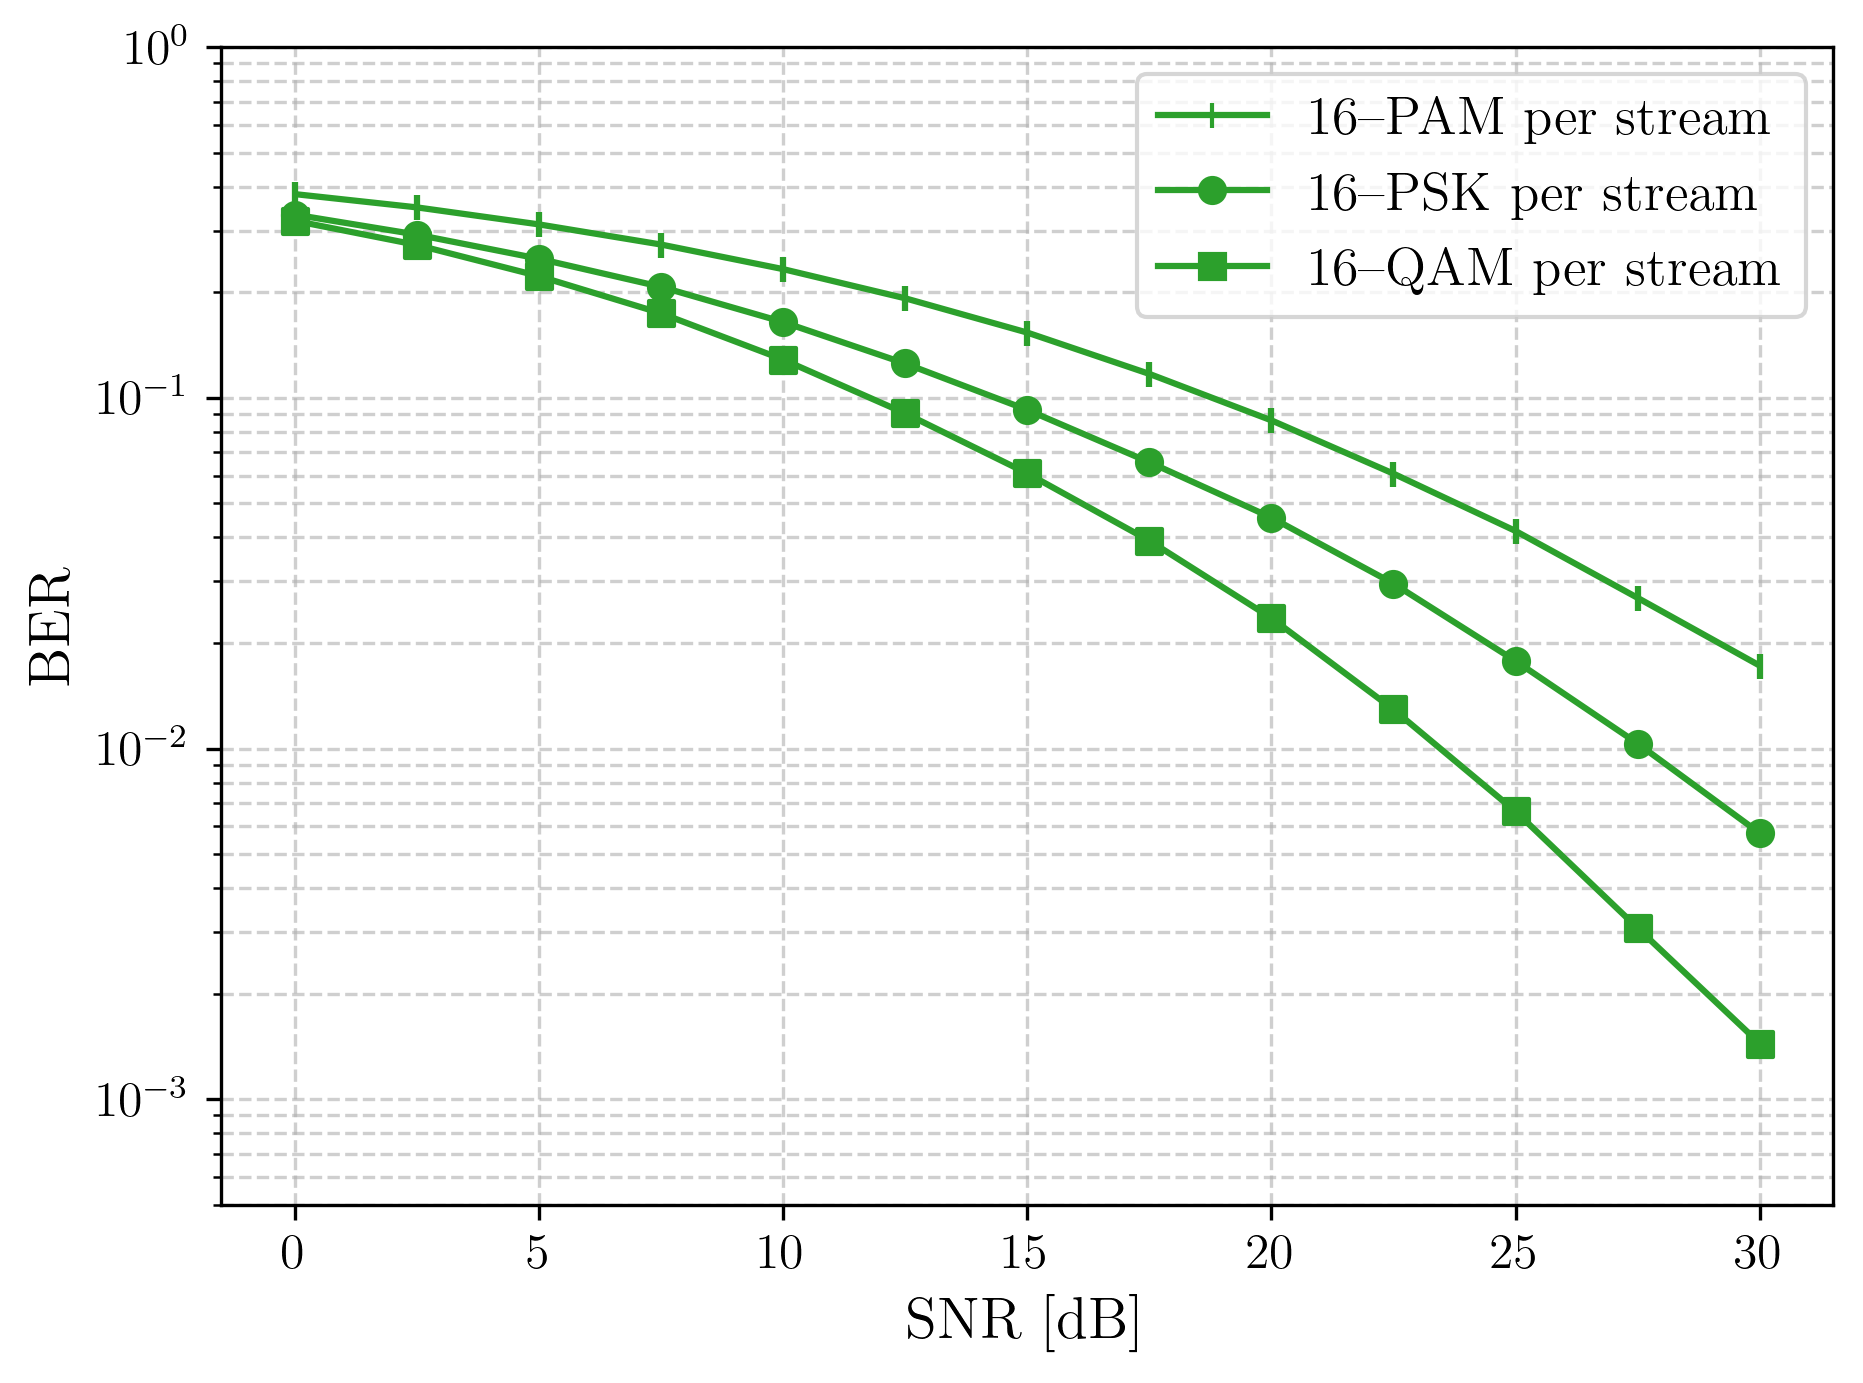
\includegraphics[width=0.55\linewidth]
    {figures/background_material/03_su_mimo_precoding/impact_constellation/2x2_fixed_ba_ber_vs_snr.png}
    \caption[System performance with fixed bit allocation]
    {\ac{BER} as a function of \ac{SNR} for three \ac{SU}-\ac{MIMO} systems with $2$ transmit and $2$ receive antennas, each using different modulation constellations on each stream: 16--\ac{PAM}, 16--\ac{PSK}, and 16--\ac{QAM}.}
    \label{fig:impact_constellation_2x2_fixed_ba_ber_vs_snr}
\end{figure}

As established in Section~\ref{section:maximum_information_rate_design}, the maximum information rate design is particularly relevant in adaptive modulation systems, where the number of bits per symbol is not fixed but adapted to the instantaneous capacity of each eigen subchannel.
Specifically, the bit allocation on subchannel $i$ is set to the largest even integer not exceeding its capacity.
Figure~\ref{fig:adaptive_ba_4x4_QAM_optimal_pa_r_100} illustrates the resulting bit allocations for a $4 \times 4$ system at two different \ac{SNR} values.
At low \ac{SNR}, the waterfilling solution concentrates almost all power on the strongest eigen subchannel, which is the only one capable of supporting a non-zero bit allocation.
Because waterfilling maximizes the mutual information without accounting for the discrete nature of the bit allocation, a small amount of power is still directed to the weaker subchannels.
Since their capacities fall below the $2$-bit threshold, however, their bit allocations remain zero and the corresponding power is wasted.
Jointly optimizing the power and bit allocation to avoid this inefficiency has been studied in~\cite{mercury_waterfilling, practical_bit_loading}, but is not considered in this dissertation.
At high \ac{SNR}, more subchannels become active and support higher-order constellations, increasing the total \ac{IBR}.

\begin{figure}[htb]
    \centering
    \begin{subfigure}[c]{0.495\textwidth}
        \centering
        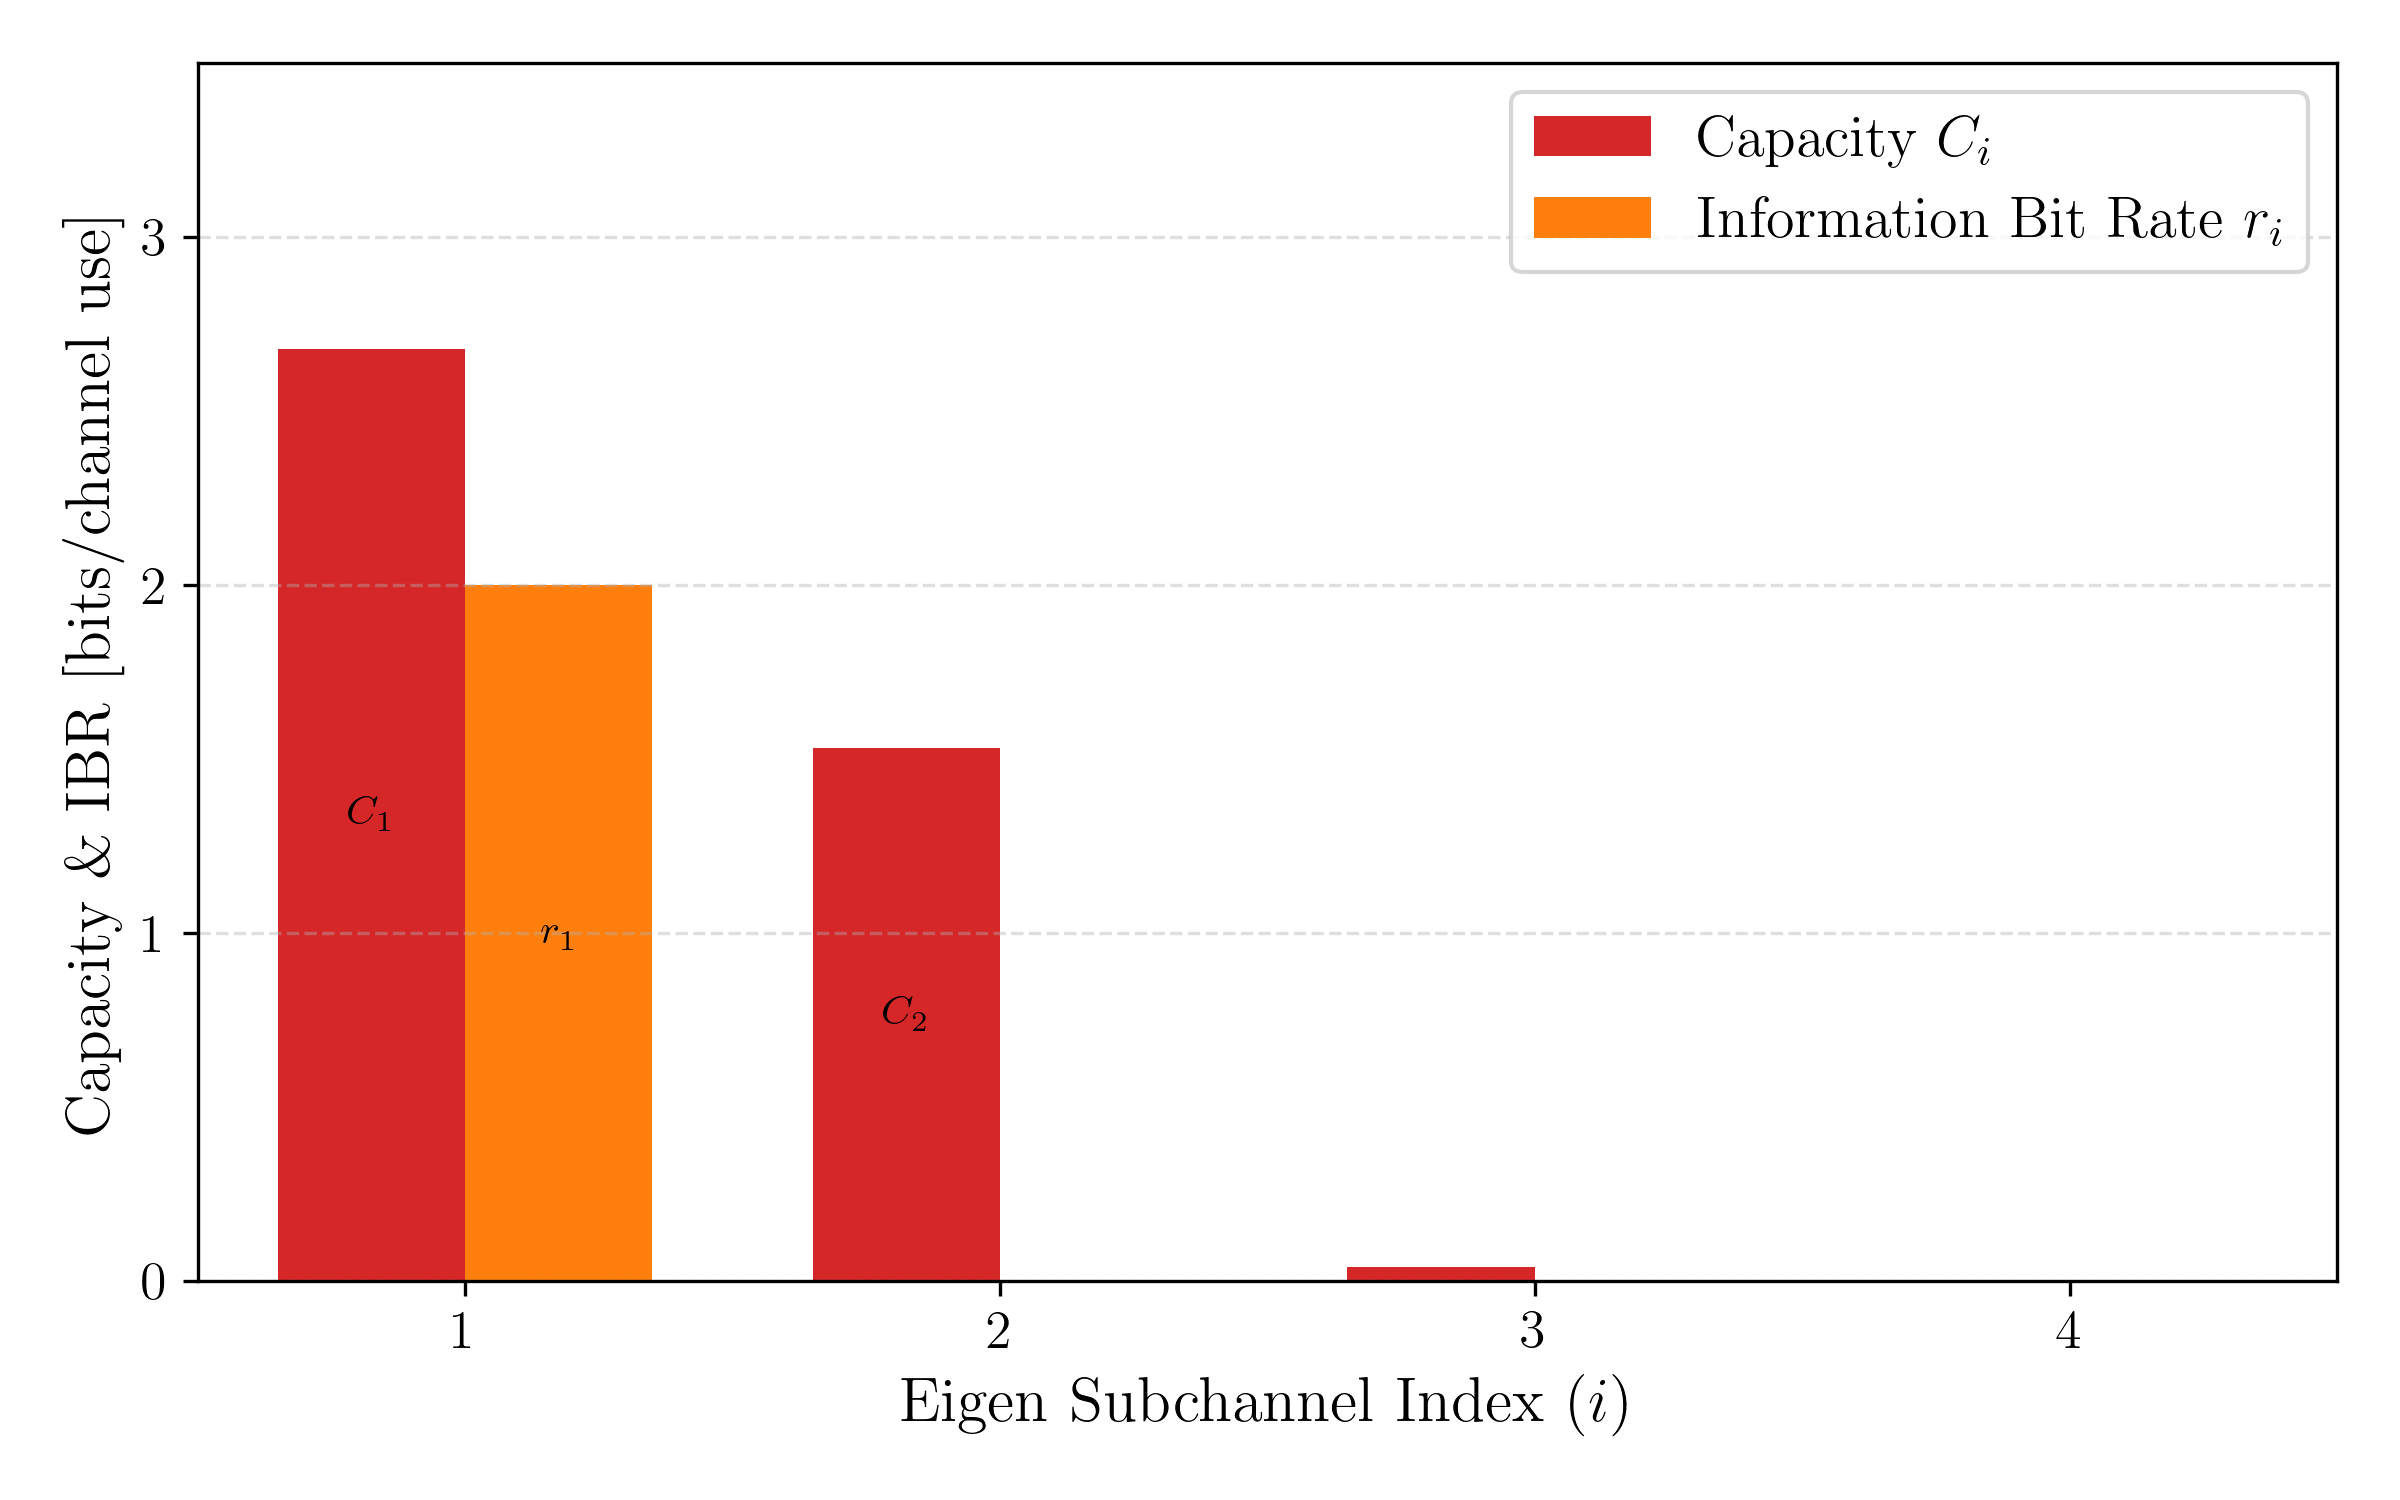
\includegraphics[width=\linewidth]
        {figures/background_material/03_su_mimo_precoding/adaptive_ba/4x4_QAM_optimal_pa_r_100_snr_0dB.png}
        \caption{$0 \, \mathrm{dB}$}
        \label{subfig:adaptive_ba_4x4_QAM_optimal_pa_r_100_snr_0dB}
    \end{subfigure}
    \hfill
    \begin{subfigure}[c]{0.495\textwidth}
        \centering
        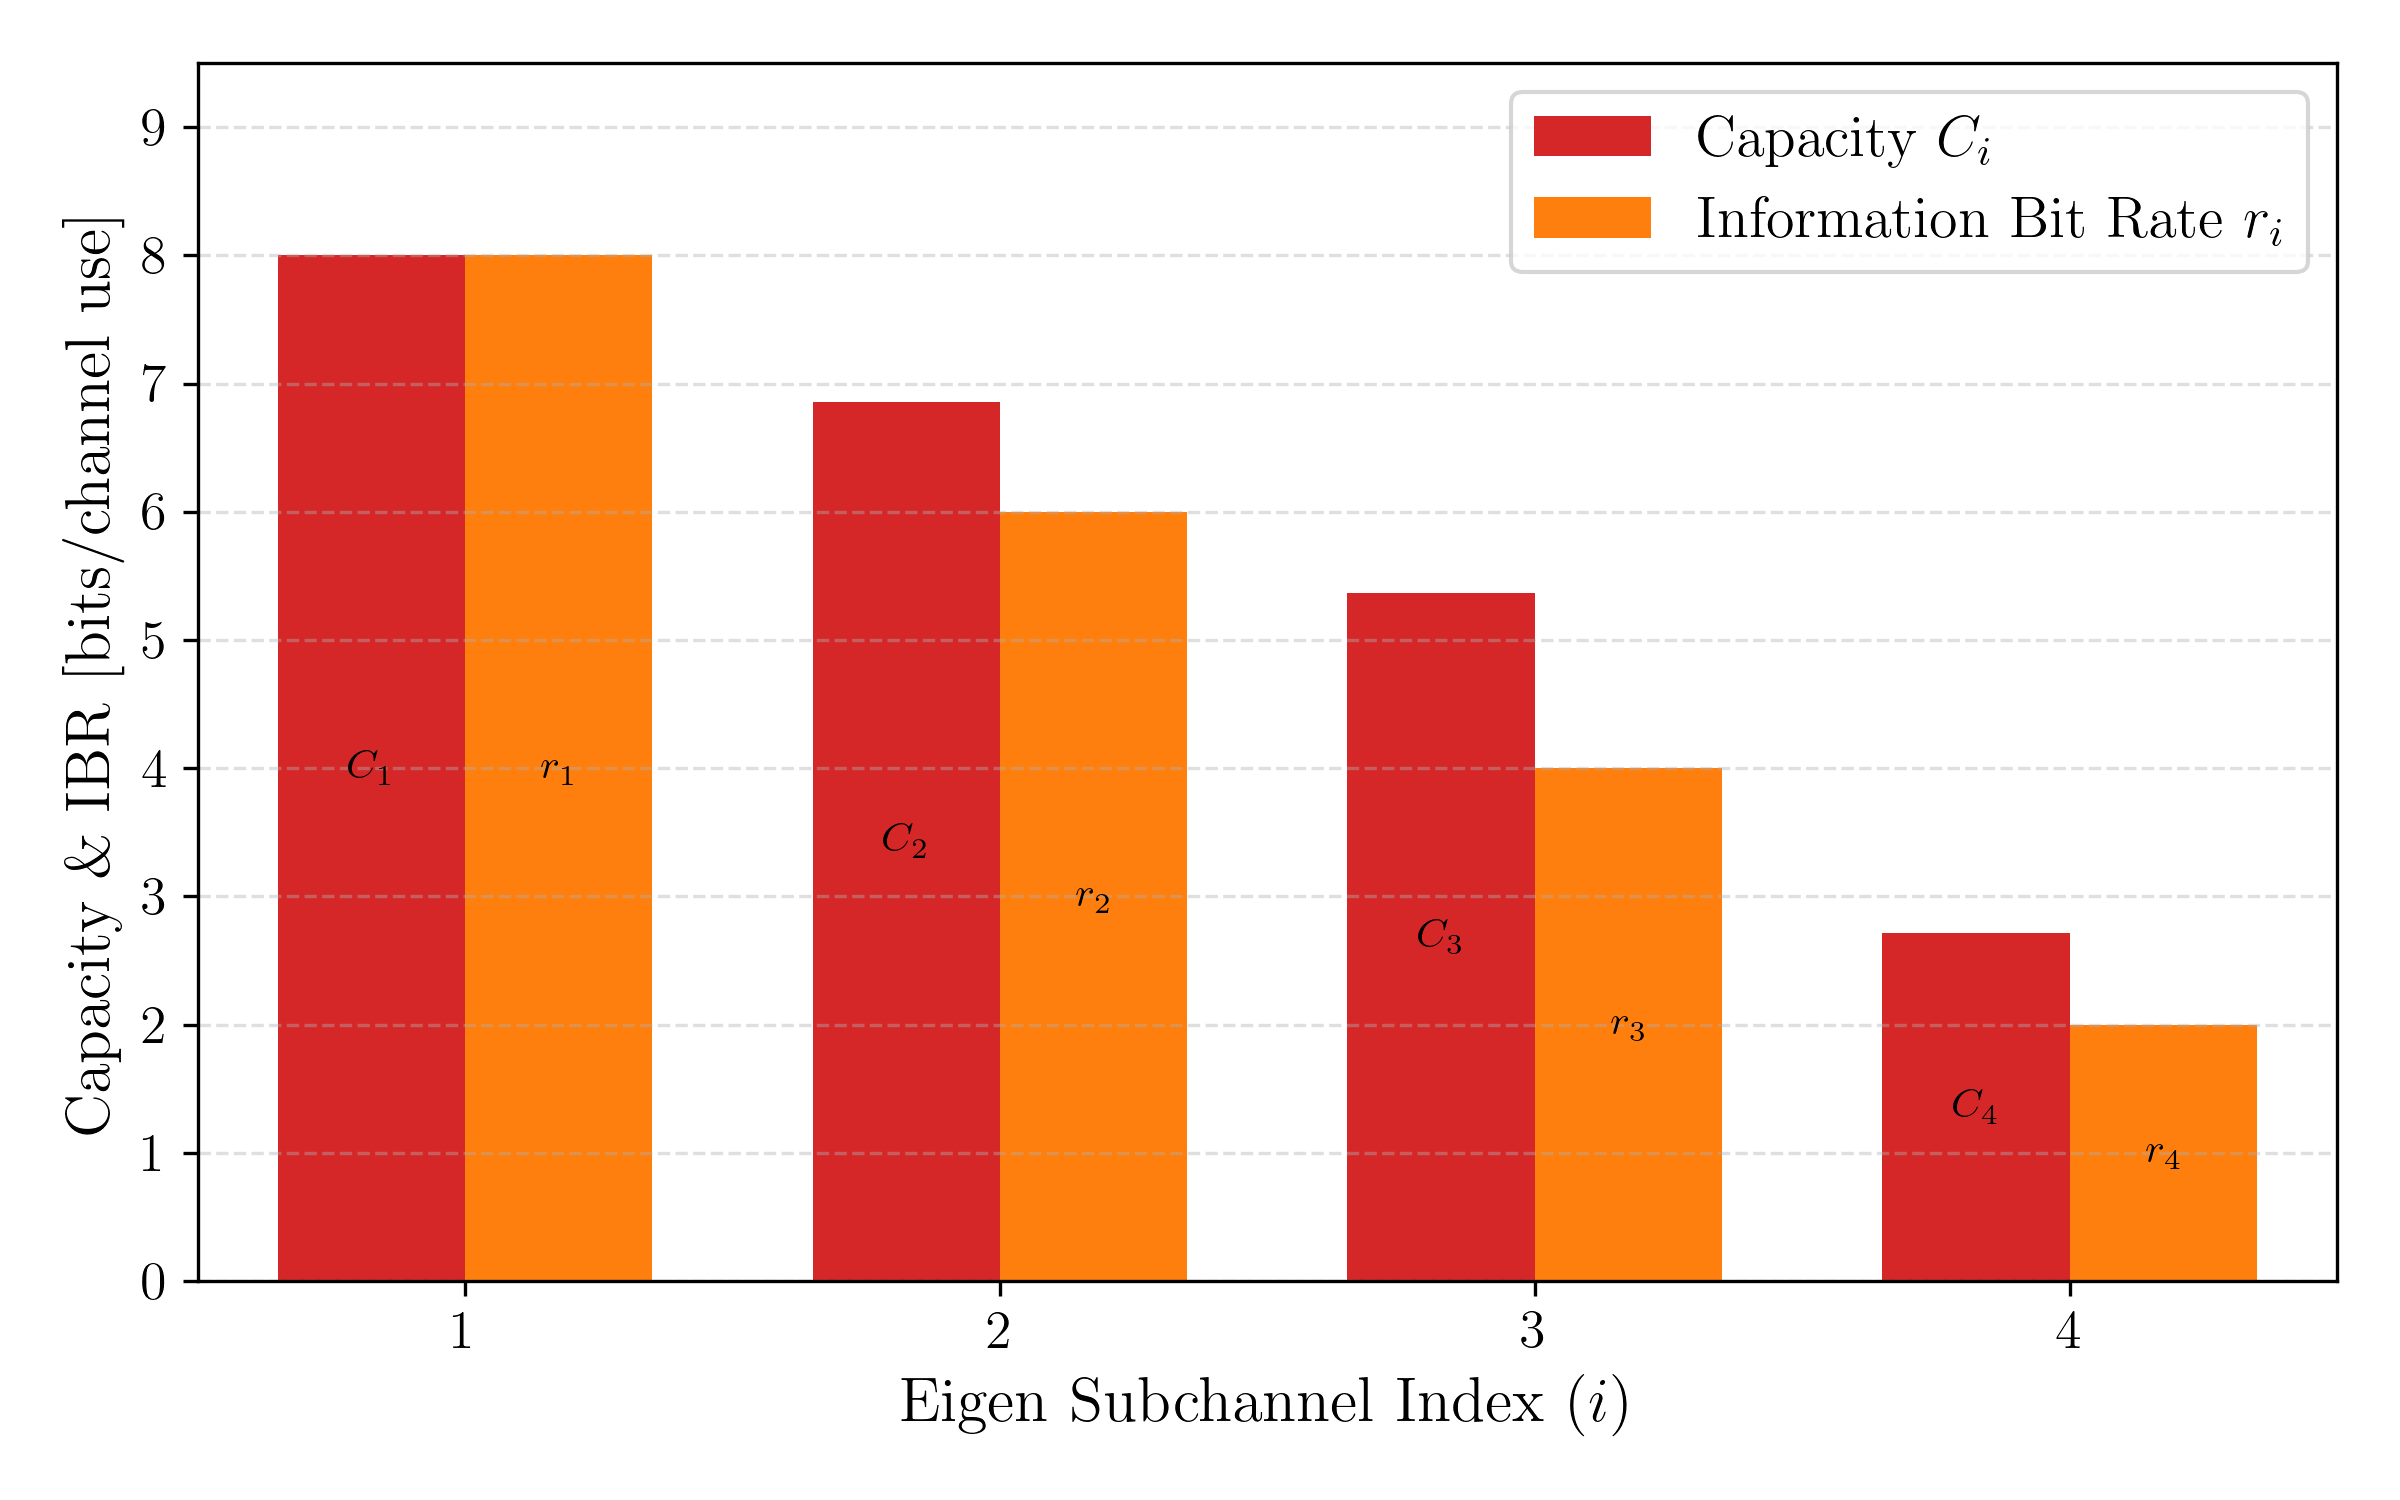
\includegraphics[width=\linewidth]
        {figures/background_material/03_su_mimo_precoding/adaptive_ba/4x4_QAM_optimal_pa_r_100_snr_20dB.png}
        \caption{$20 \, \mathrm{dB}$}
        \label{subfig:adaptive_ba_4x4_QAM_optimal_pa_r_100_snr_20dB}
    \end{subfigure}
    \caption[Adaptive bit allocation in different SNR regimes]
    {Adaptive bit allocation in different \ac{SNR} regimes for a system with $4$ transmit and $4$ receive antennas. The number of bits per symbol on each stream is the largest even integer not exceeding the capacity of the corresponding eigen subchannel.}
    \label{fig:adaptive_ba_4x4_QAM_optimal_pa_r_100}
\end{figure}

Figure~\ref{fig:impact_constellation_4x4_adaptive_ba} shows the \ac{BER} and \ac{IBR} as a function of \ac{SNR} for this adaptive bit allocation strategy.
In contrast to the fixed bit allocation case, the \ac{BER} remains approximately constant across the entire \ac{SNR} range, while the \ac{IBR} increases steadily with \ac{SNR}, as expected.

\begin{figure}[htb]
    \centering
    \begin{subfigure}[c]{0.495\textwidth}
        \centering
        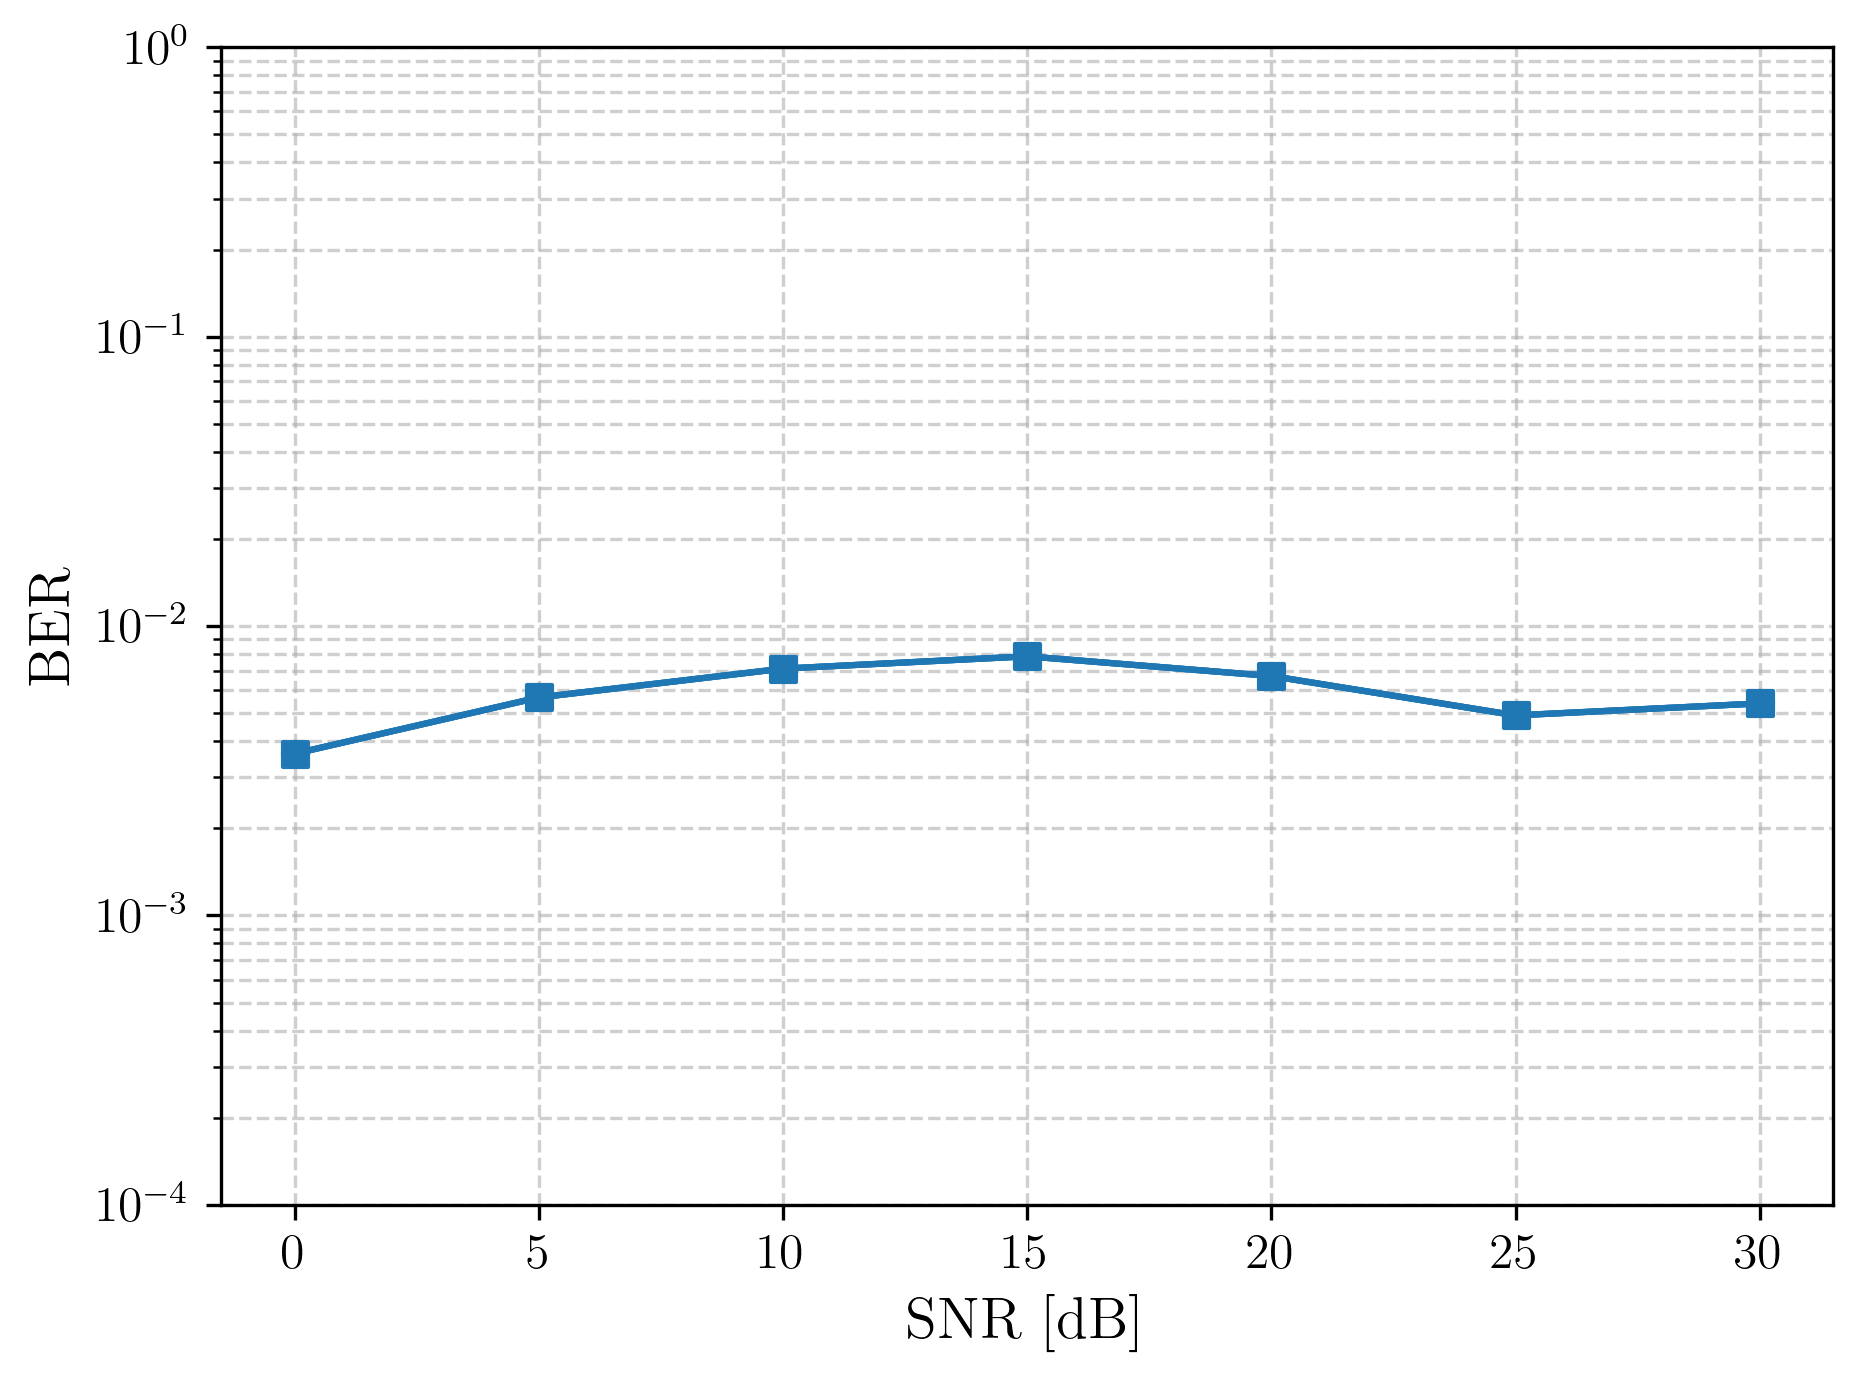
\includegraphics[width=\linewidth]
        {figures/background_material/03_su_mimo_precoding/impact_constellation/4x4_adaptive_ba_ber_vs_snr.png}
        \caption{}
        \label{subfig:impact_constellation_4x4_adaptive_ba_ber_vs_snr}
    \end{subfigure}
    \hfill
    \begin{subfigure}[c]{0.495\textwidth}
        \centering
        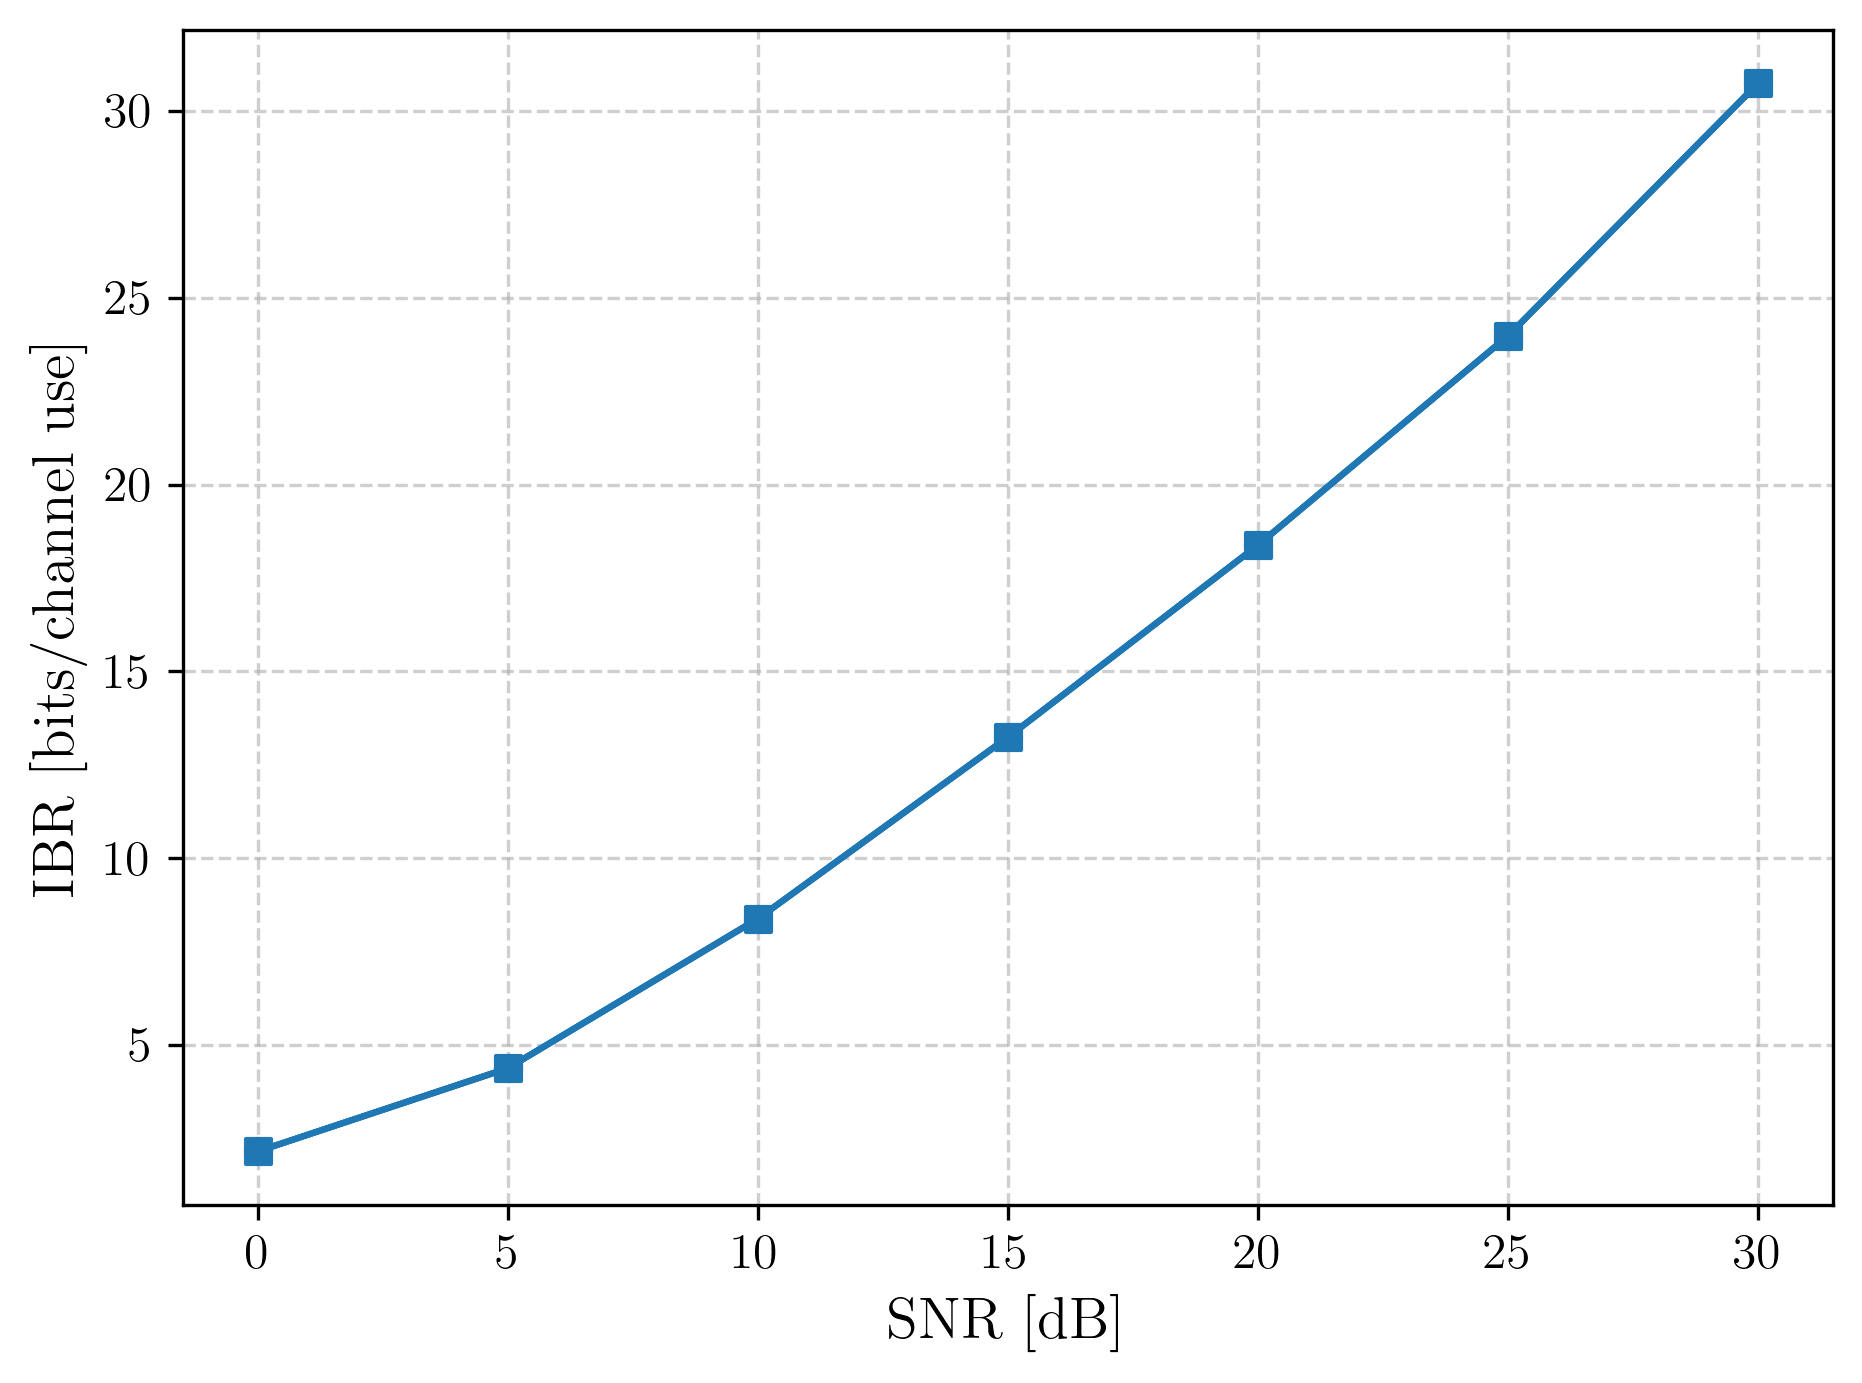
\includegraphics[width=\linewidth]
        {figures/background_material/03_su_mimo_precoding/impact_constellation/4x4_adaptive_ba_ibr_vs_snr.png}
        \caption{}
        \label{subfig:impact_constellation_4x4_adaptive_ba_ibr_vs_snr}
    \end{subfigure}
    \caption[System performance with adaptive bit allocation]
    {System performance with adaptive bit allocation for a system with $4$ transmit and $4$ receive antennas. The \ac{BER} and \ac{IBR} are shown as a function of \ac{SNR}.}
    \label{fig:impact_constellation_4x4_adaptive_ba}
\end{figure}

\subsection{Impact of the Data Rate}
\label{subsection:impact_of_information_bit_rate}
% =========================================
%    Impact of the Data Rate
% =========================================

The previous subsection assigned to each eigen subchannel the largest even number of bits not exceeding the subchannel capacity, so that the system operated at approximately the maximum achievable rate.
In practice, however, it may be preferable to transmit at a lower rate in exchange for a reduced \ac{BER}.
To quantify this trade-off, we introduce a rate factor $r_f \in (0, 1]$ that specifies which fraction of the subchannel capacity is used for transmission.
The bit allocation on subchannel $i$ is then generalized to the largest even integer not exceeding $r_f \, C_i$, where $C_i$ denotes the instantaneous capacity of that subchannel.
The case $r_f = 1$ recovers the maximum-rate allocation of the previous subsection.

\begin{figure}[bht]
    \centering
    \begin{subfigure}[c]{0.495\textwidth}
        \centering
        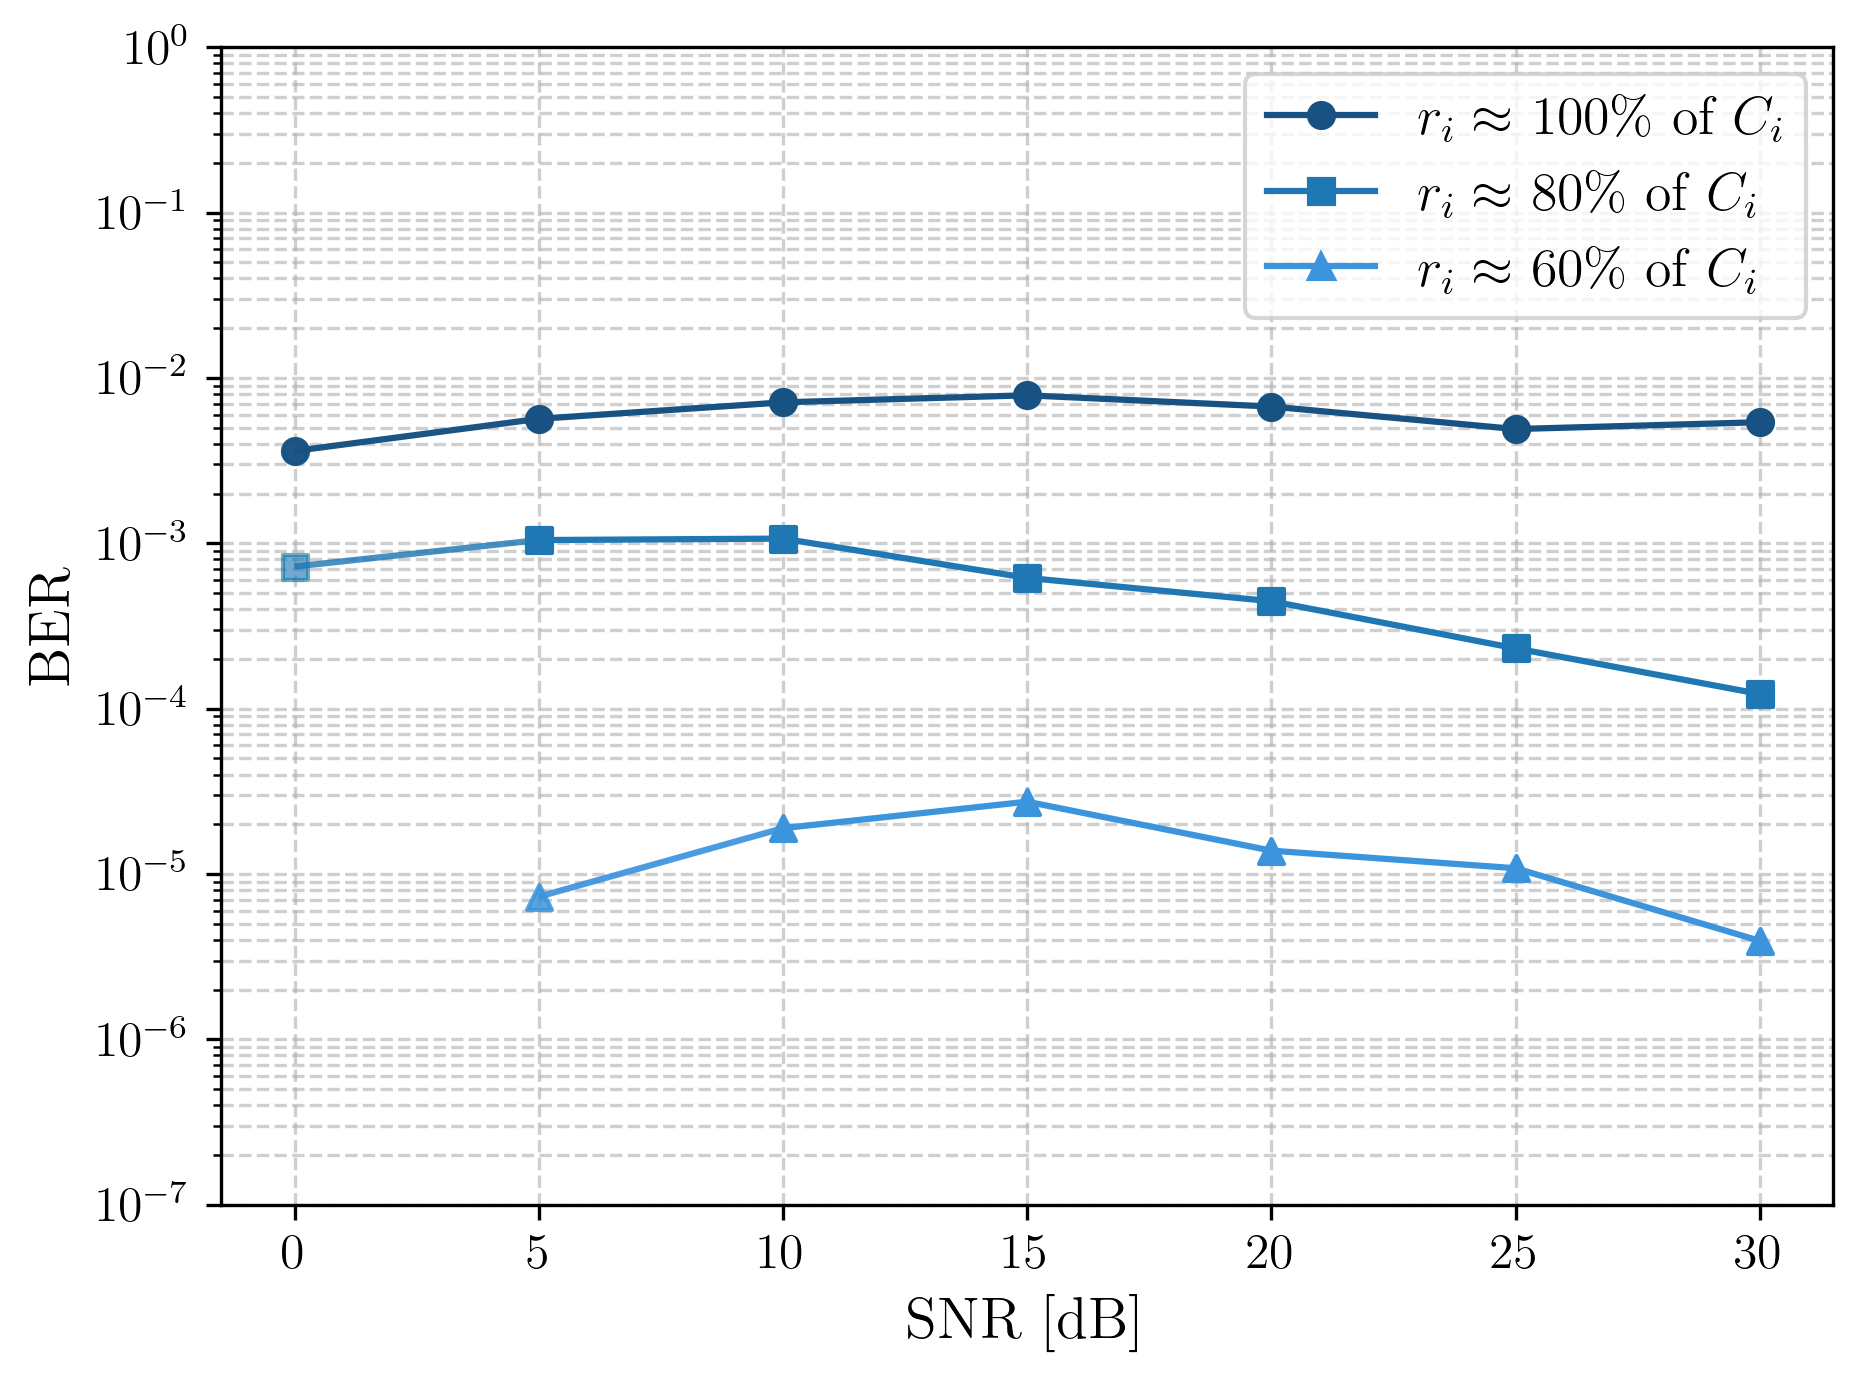
\includegraphics[width=\linewidth]
        {figures/background_material/03_su_mimo_precoding/impact_ibr/4x4_adaptive_ba_ber_vs_snr.png}
        \caption{}
        \label{subfig:impact_ibr_4x4_adaptive_ba_ber_vs_snr}
    \end{subfigure}
    \hfill
    \begin{subfigure}[c]{0.495\textwidth}
        \centering
        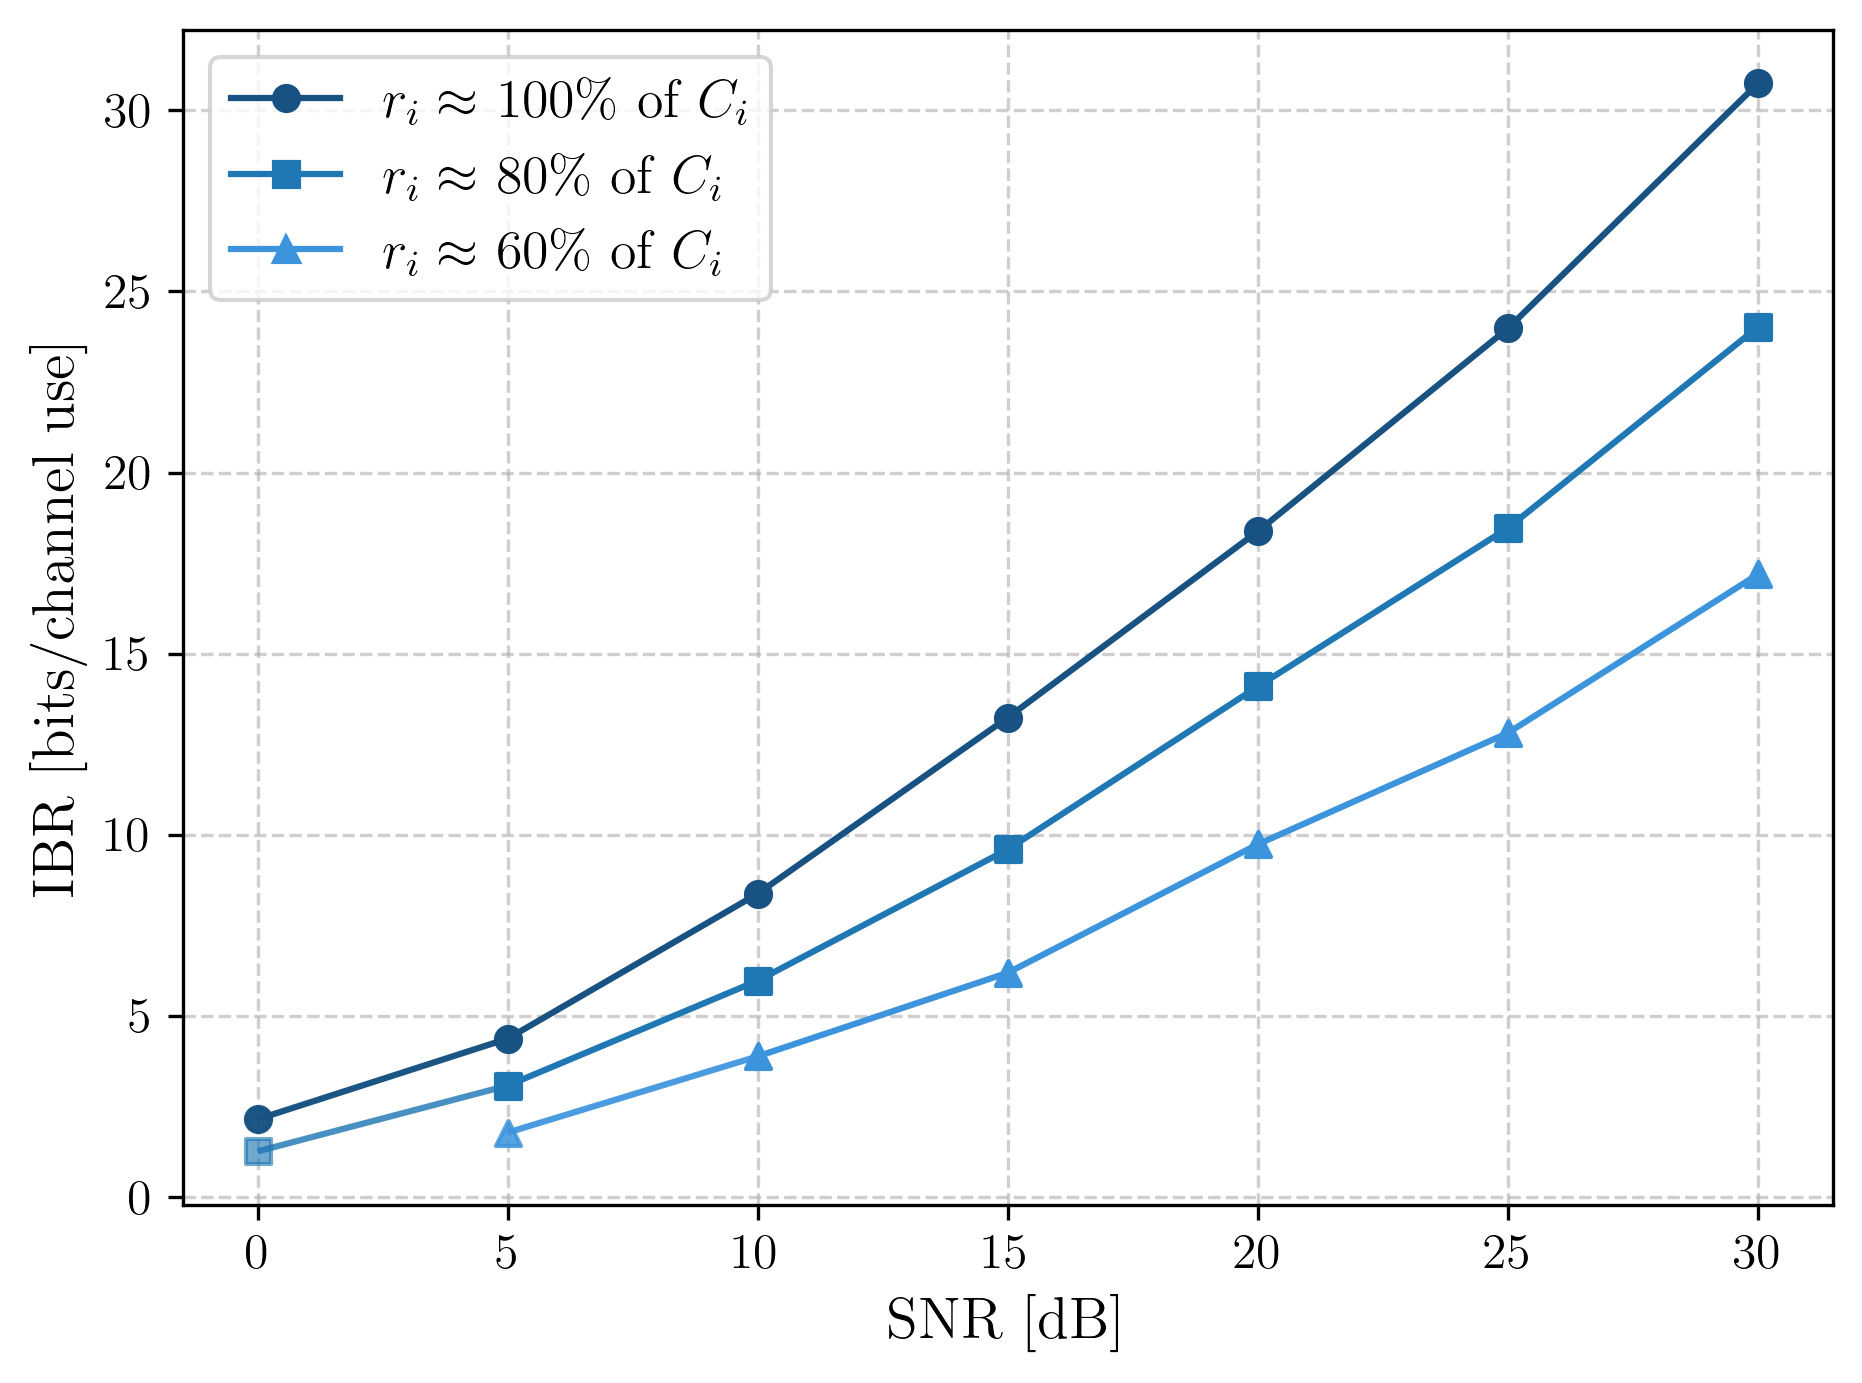
\includegraphics[width=\linewidth]
        {figures/background_material/03_su_mimo_precoding/impact_ibr/4x4_adaptive_ba_ibr_vs_snr.png}
        \caption{}
        \label{subfig:impact_ibr_4x4_adaptive_ba_ibr_vs_snr}
    \end{subfigure}
    \caption[Impact of the IBR on the system performance (adaptive bit allocation)]
    {Illustration of the impact of the data rate on the system performance for a system with $4$ transmit and $4$ receive antennas using adaptive bit allocation. The (a) \ac{BER} and (b) \ac{IBR} are shown as a function of \ac{SNR}, for three different rate factors.}
    \label{fig:impact_ibr_4x4_adaptive_ba}
\end{figure}

Figure~\ref{fig:impact_ibr_4x4_adaptive_ba} shows the \ac{BER} and \ac{IBR} as a function of \ac{SNR} for several values of $r_f$ on a $4 \times 4$ system.
As expected, reducing $r_f$ lowers the \ac{IBR}, because fewer bits are assigned to each subchannel.
At the same time, the \ac{BER} decreases, since the chosen modulation order moves further below the subchannel capacity and the link operates with a larger margin.
This illustrates an important trade-off between throughput and reliability: operating below capacity sacrifices data rate in exchange for improved error performance.

For completeness, Figure~\ref{fig:impact_ibr_2x2_fixed_ba_ber_vs_snr} shows the analogous experiment under fixed bit allocation on a $2 \times 2$ system, where the same modulation order is applied on all eigen subchannels across the entire \ac{SNR} range.
The behavior is consistent: a smaller constellation size yields a lower \ac{BER} at any given \ac{SNR}.
The slope of the \ac{BER} curve is essentially unchanged by the constellation order.

\begin{figure}[htb]
    \centering
    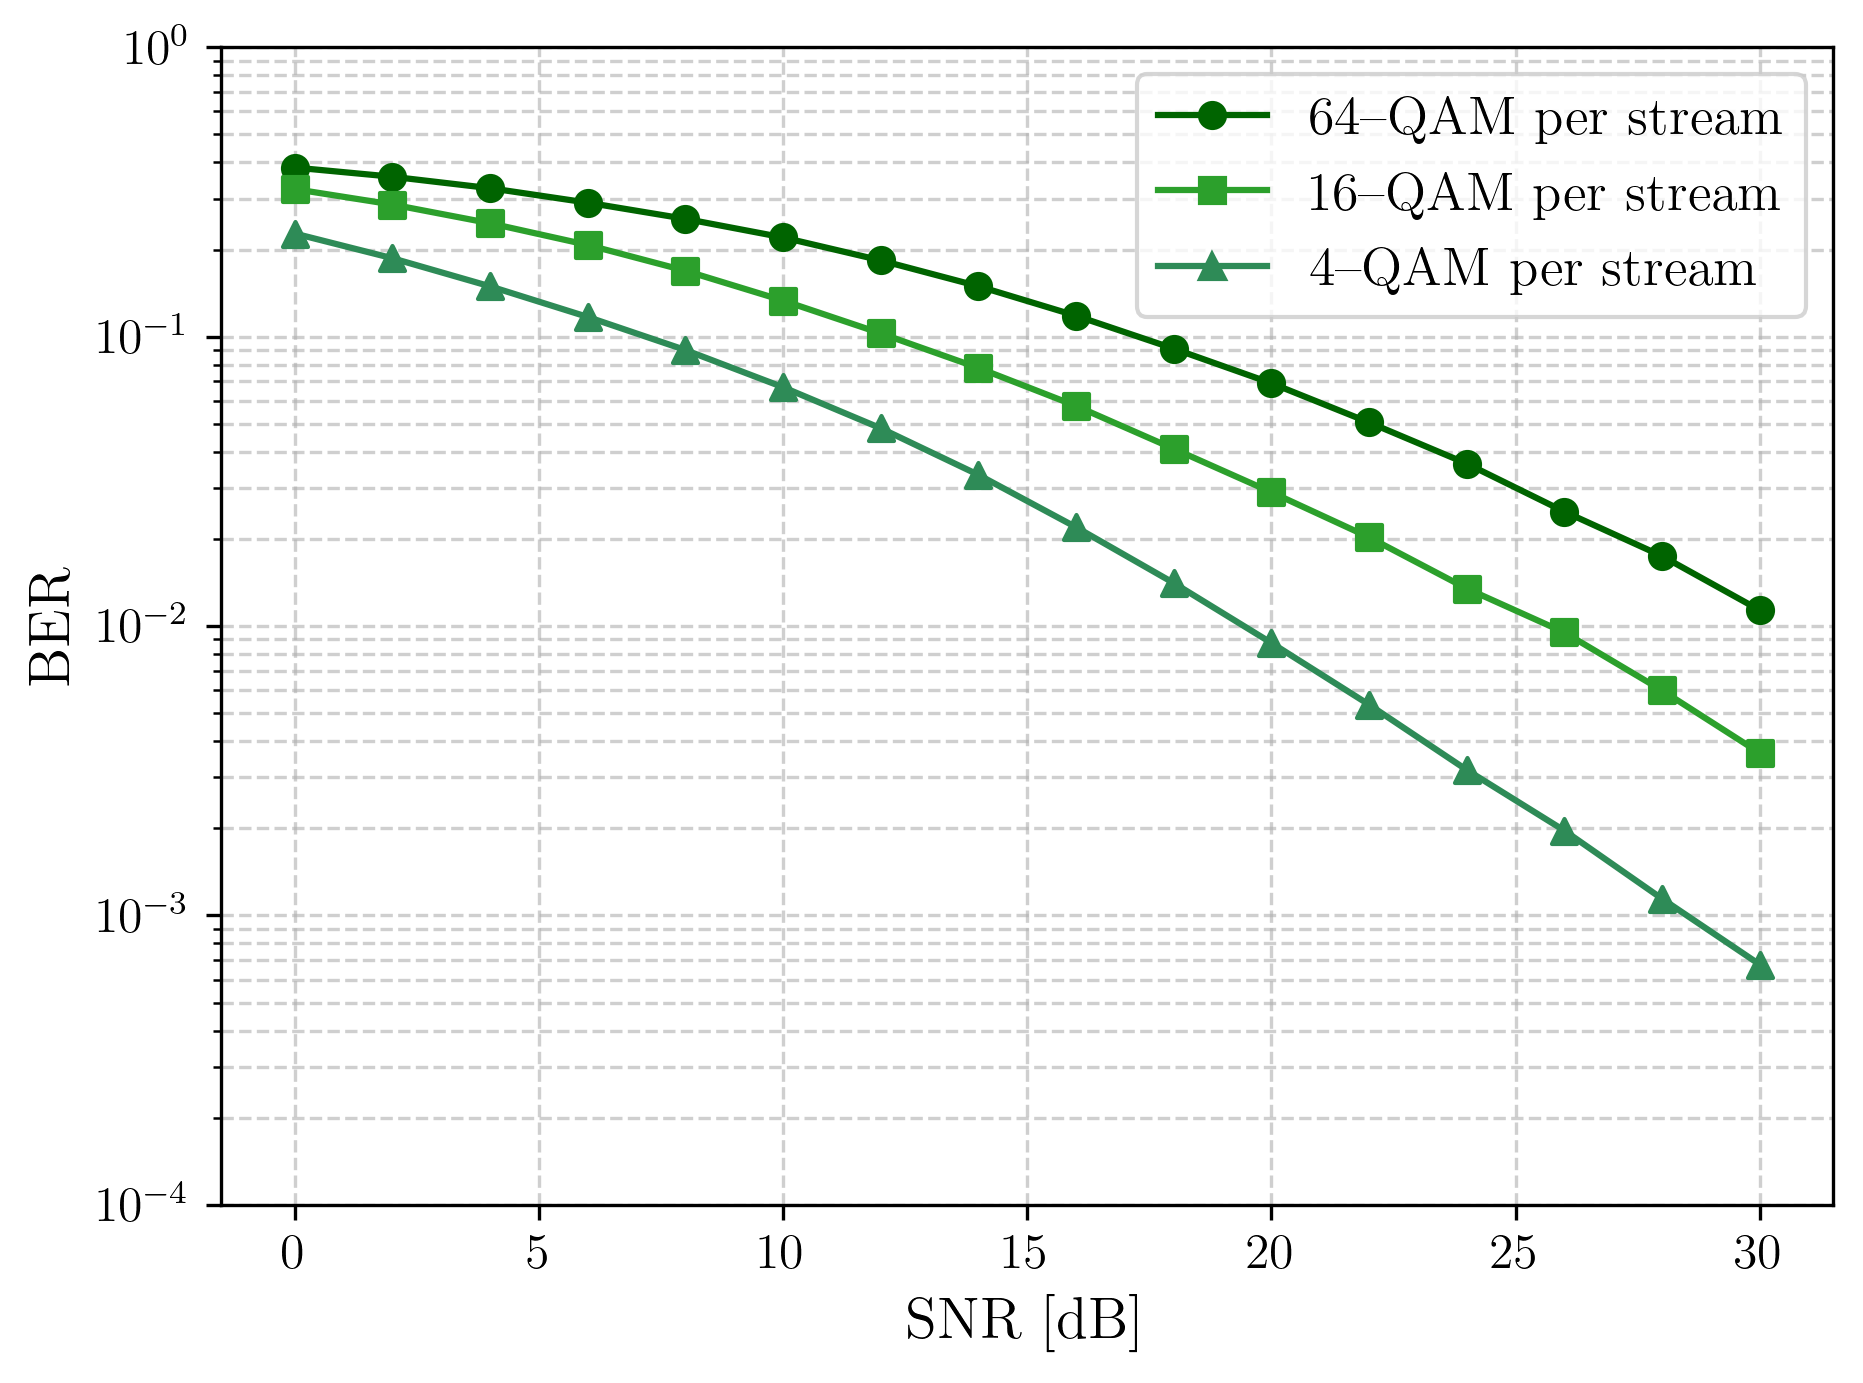
\includegraphics[width=0.55\linewidth]
    {figures/background_material/03_su_mimo_precoding/impact_ibr/2x2_fixed_ba_ber_vs_snr.png}
    \caption[Impact of the IBR on the system performance (fixed bit allocation)]
    {Illustration of the impact of the data rate on the system performance for a system with $2$ transmit and $2$ receive antennas using fixed bit allocation. The \ac{BER} is shown as a function of \ac{SNR} for three different modulation orders.}
    \label{fig:impact_ibr_2x2_fixed_ba_ber_vs_snr}
\end{figure}

\subsection{Impact of the Antenna Count}
\label{subsection:impact_of_antenna_count}
% =====================================
%    Impact of the Antenna Count
% =====================================


This subsection examines how the number of transmit and receive antennas affects system performance, keeping the rate factor fixed at $r_f = 1$.
Figure~\ref{fig:impact_antennas_variable_ibr_4x4_adaptive_ba} shows the \ac{BER} and \ac{IBR} as a function of \ac{SNR} for several antenna configurations.
The \ac{BER} remains approximately constant across all configurations, consistent with the behavior observed in Section~\ref{subsection:bit_allocation_strategies}.
By contrast, the maximum achievable rate, and thus the \ac{IBR}, varies markedly with antenna count.
Three distinct effects can be observed.

\begin{figure}[htb]
    \centering
    \begin{subfigure}[c]{0.495\textwidth}
        \centering
        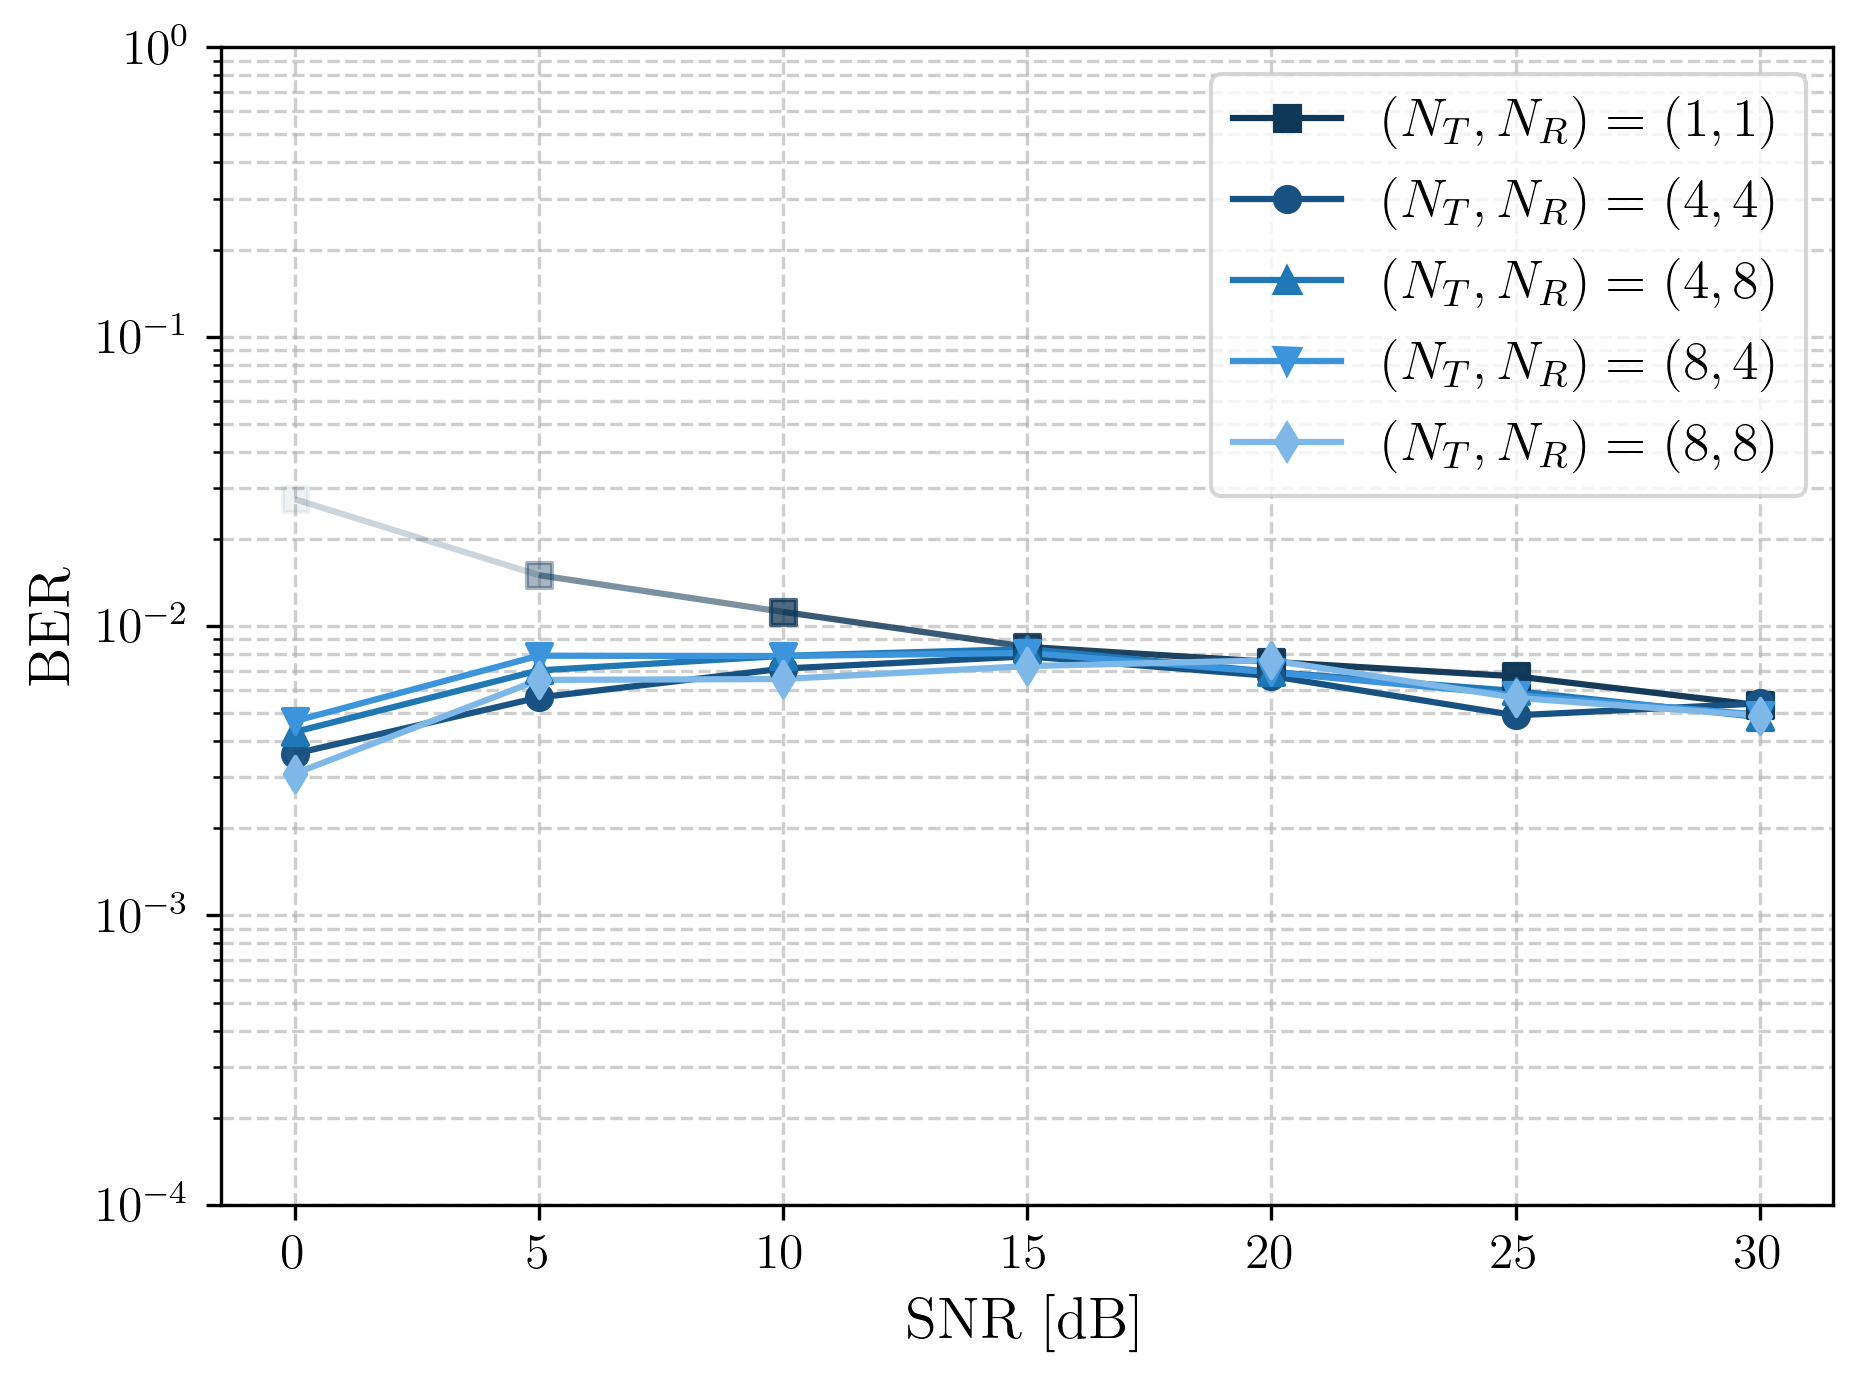
\includegraphics[width=\linewidth]
        {figures/background_material/03_su_mimo_precoding/impact_antennas/variable_ibr_ber_vs_snr.png}
        \caption{}
        \label{subfig:impact_antennas_variable_ibr_4x4_adaptive_ba_ber_vs_snr}
    \end{subfigure}
    \hfill
    \begin{subfigure}[c]{0.495\textwidth}
        \centering
        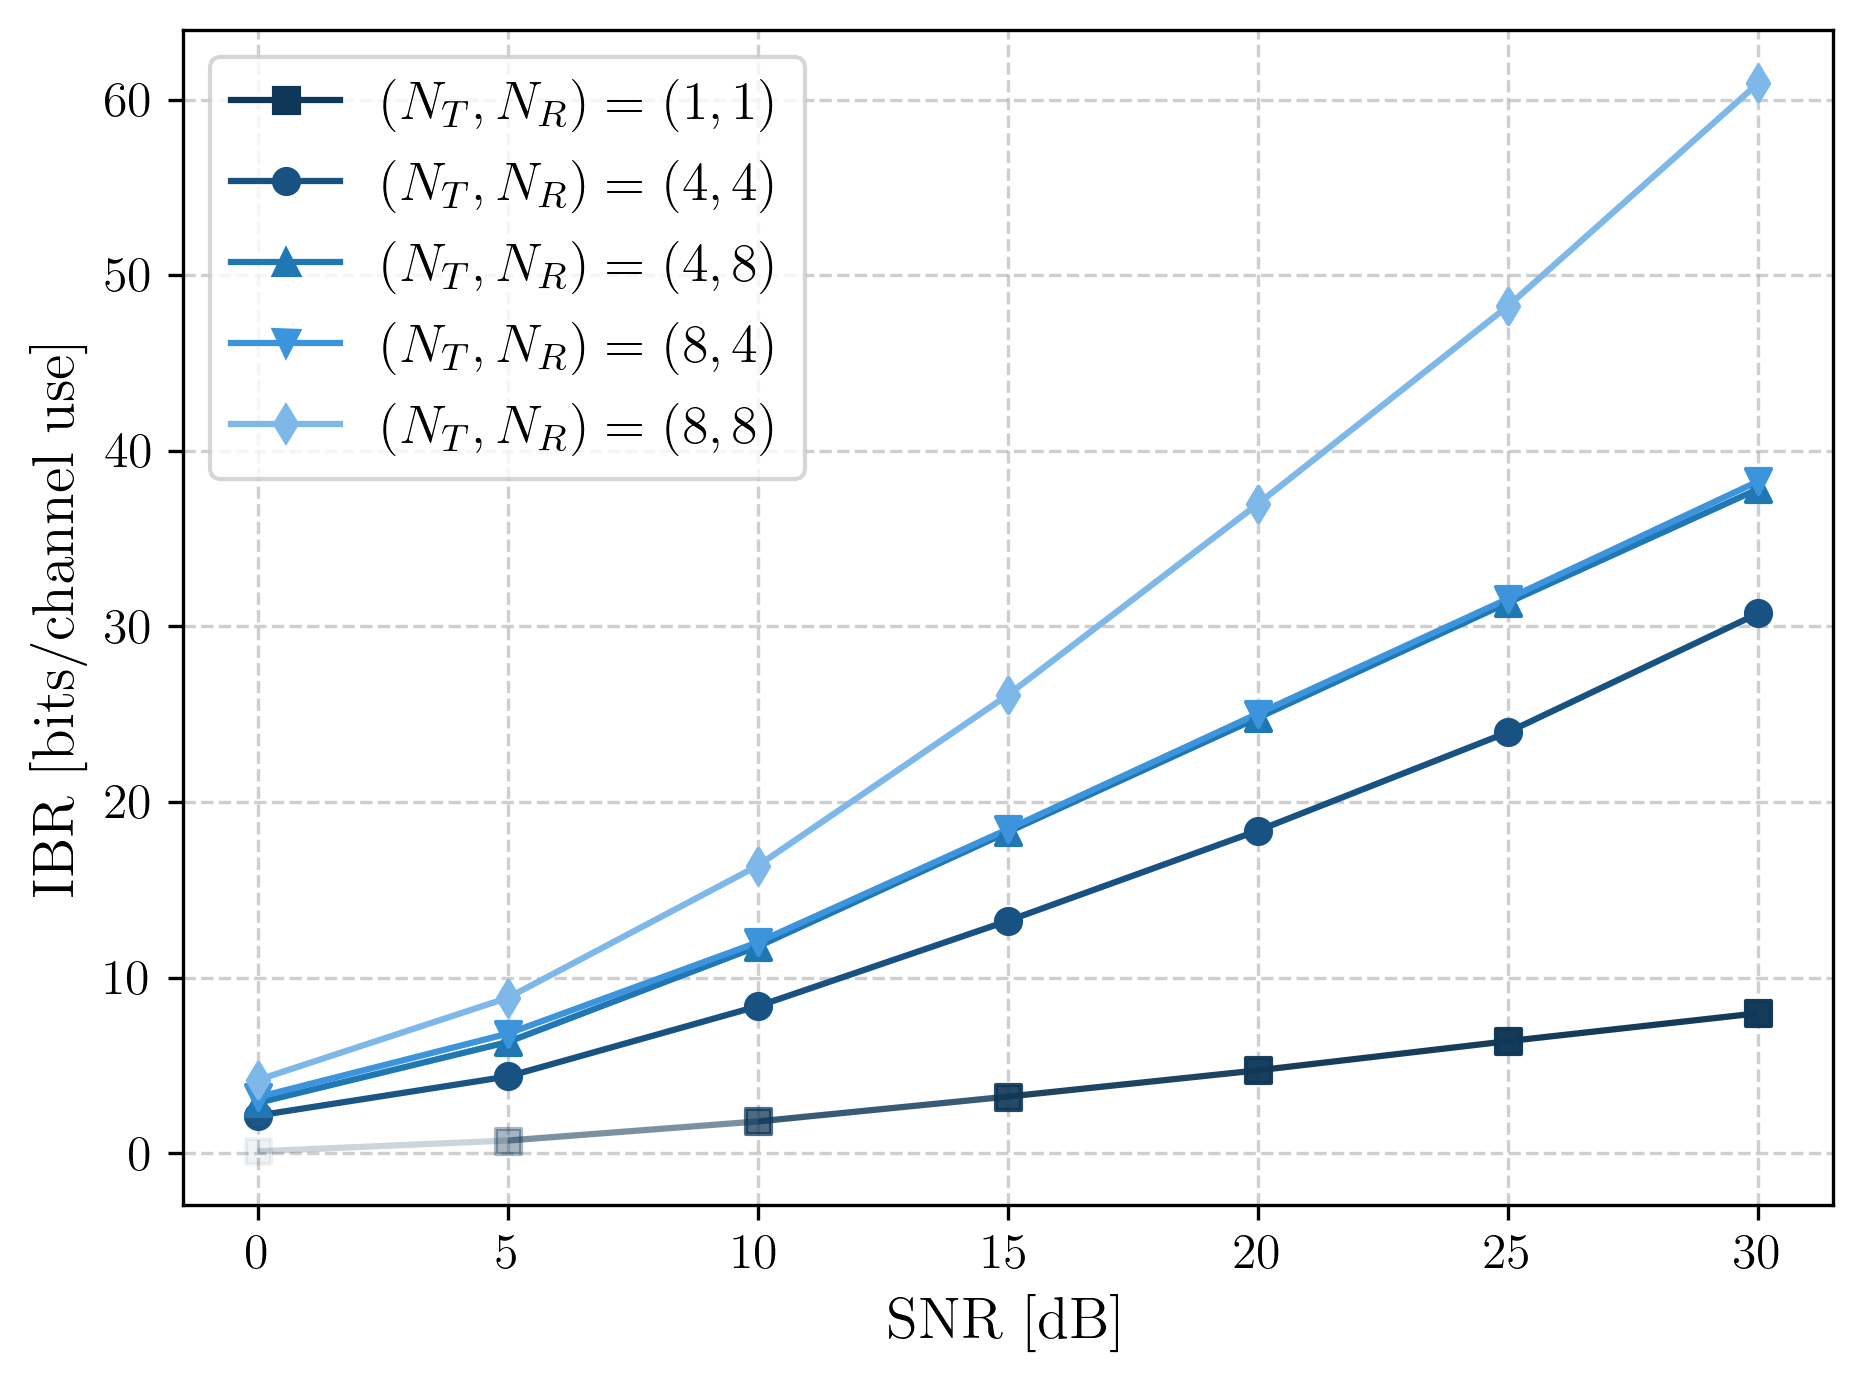
\includegraphics[width=\linewidth]
        {figures/background_material/03_su_mimo_precoding/impact_antennas/variable_ibr_ibr_vs_snr.png}
        \caption{}
        \label{subfig:impact_antennas_variable_ibr_4x4_adaptive_ba_ibr_vs_snr}
    \end{subfigure}
    \caption[Impact of the antenna count on the system performance (constant BER comparison)]
    {Illustration of the impact of the antenna count on the system performance for a system using adaptive bit allocation. The (a) \ac{BER} and (b) \ac{IBR} are shown as a function of \ac{SNR}, for five different antenna configurations.}
    \label{fig:impact_antennas_variable_ibr_4x4_adaptive_ba}
\end{figure}

The first effect is a change in the slope of the \ac{IBR} curve, which is determined by $\min(N_T, N_R)$.
This follows directly from the channel rank: for an i.i.d. Rayleigh fading channel, $R_H \leq \min(N_T, N_R)$, so the number of parallel eigen subchannels cannot exceed the smaller antenna count.
Consequently, adding antennas on both sides creates additional parallel streams and therefore increases the slope of the maximum achievable rate in function of the \ac{SNR}

The second effect is a vertical upward shift of the \ac{IBR} curve when antennas are added only on the side with a larger antenna count while $\min(N_T, N_R)$ remains unchanged.
This shift occurs because, for a fixed smaller dimension, the expected values of the squared singular values of an $N_R \times N_T$ i.i.d. Gaussian matrix increase with the larger dimension~\cite{singular_values_distribution}.
The eigen subchannels thus experience better average channel conditions, yielding a higher \ac{IBR} at the same \ac{SNR} while leaving the slope unchanged.

Finally, configurations with the same $\min(N_T, N_R)$ and the same total number of antennas show no performance difference when the excess antennas are placed at the \ac{TX} or at the \ac{RX}.
This symmetry follows since $\mathbf{H}\mathbf{H}^{\mathsf{H}}$ and $\mathbf{H}^{\mathsf{H}}\mathbf{H}$ have the same non-zero eigenvalues, so the singular-value distribution of an $N_R \times N_T$ i.i.d. Rayleigh channel is identical to that of its transpose.

As in the previous subsection, the rate--reliability trade-off also applies here.
Figure~\ref{fig:impact_antennas_variable_ber_4x4_adaptive_ba} illustrates this by adjusting the rate factor of each configuration so that all systems achieve approximately the same \ac{IBR} at each \ac{SNR}.
Under this equal-rate comparison, systems with more antennas consistently achieve lower \ac{BER}, because the additional spatial degrees of freedom support the same throughput with larger margins on the individual eigen subchannels.

\begin{figure}[htb]
    \centering
    \begin{subfigure}[c]{0.495\textwidth}
        \centering
        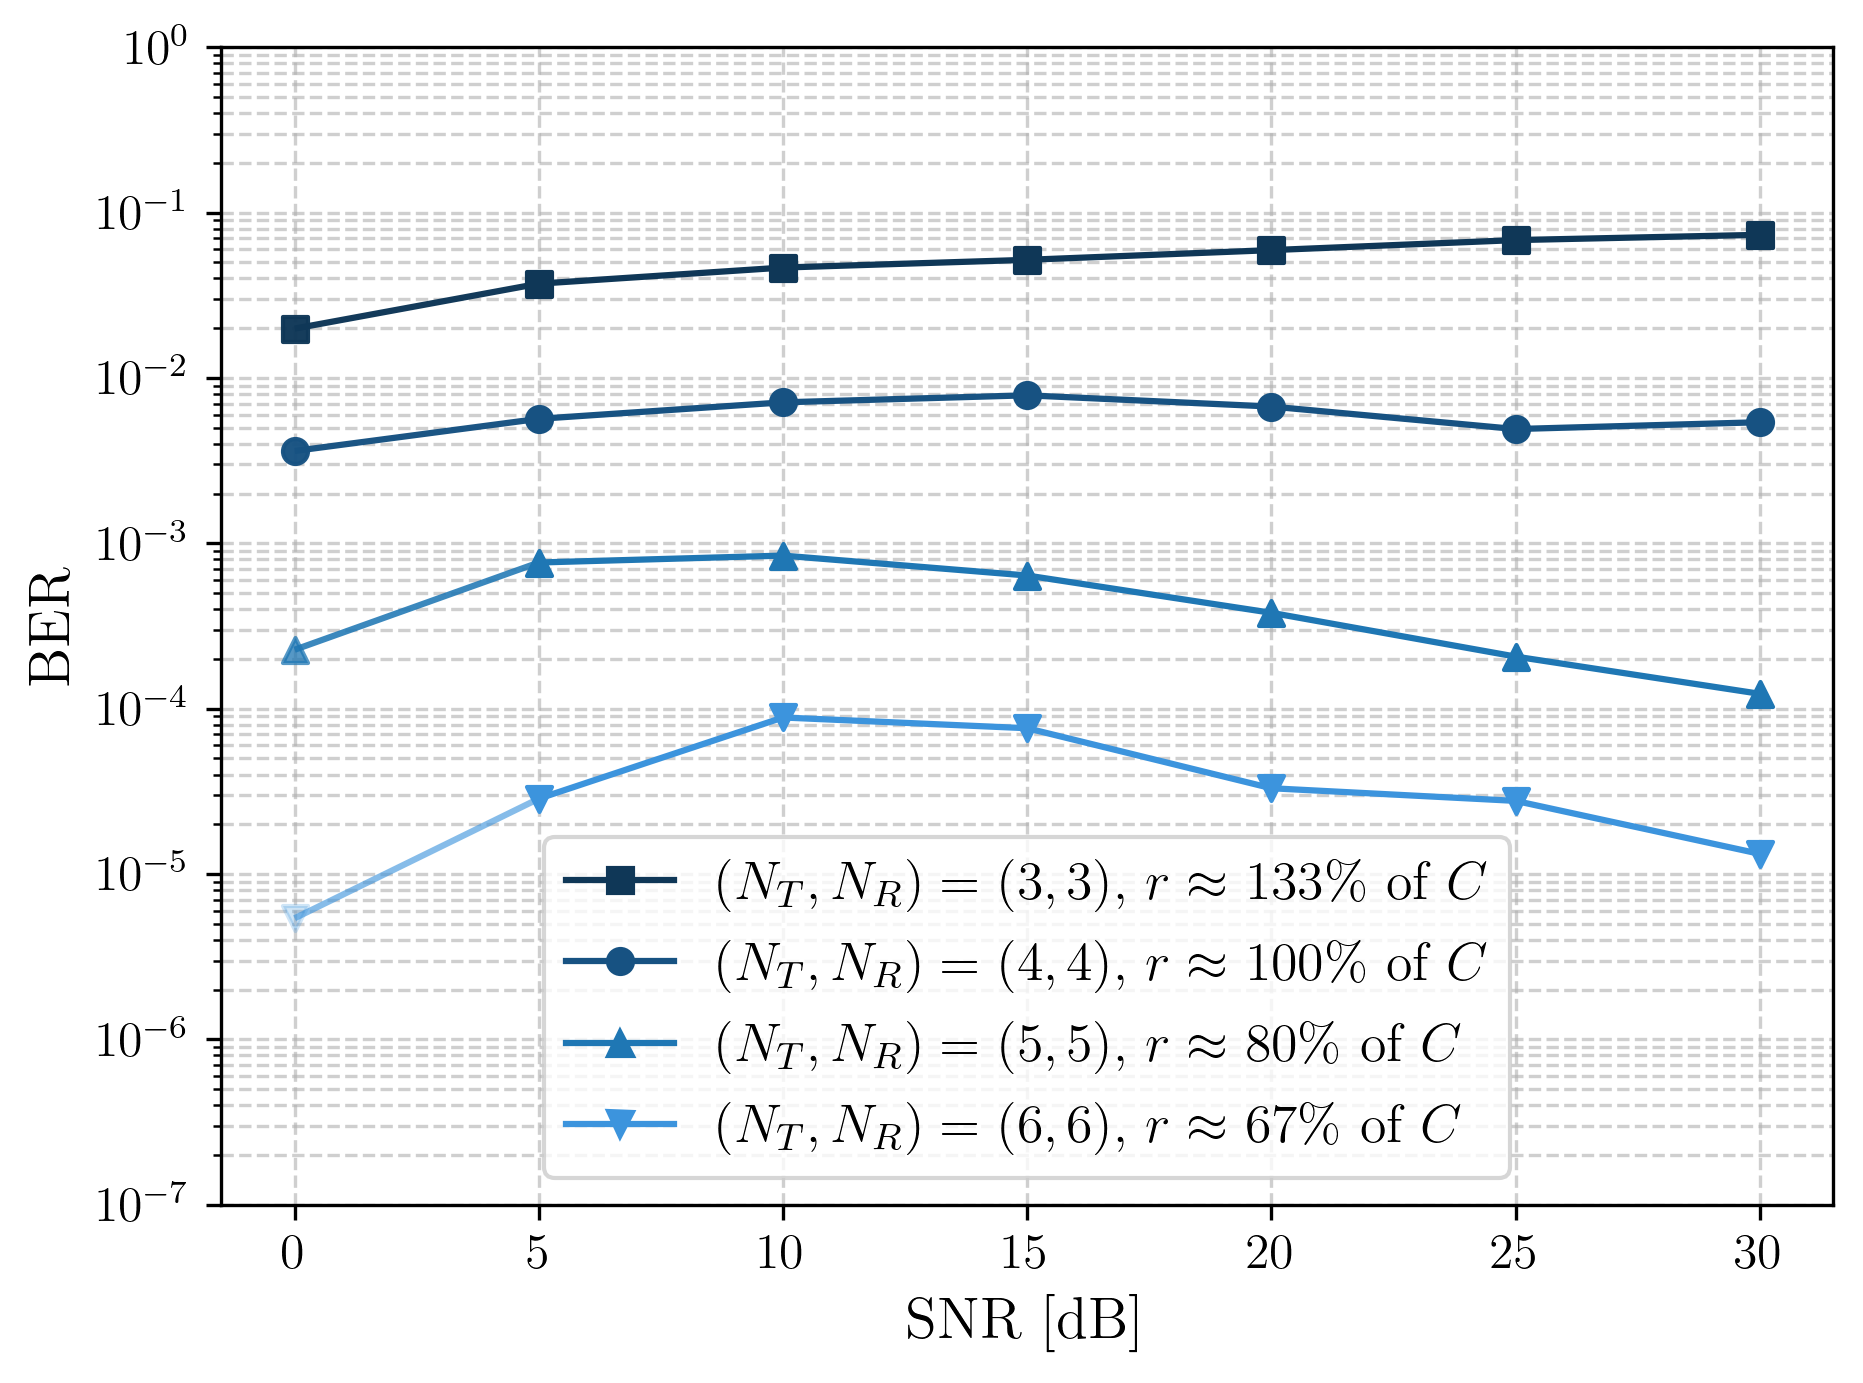
\includegraphics[width=\linewidth]
        {figures/background_material/03_su_mimo_precoding/impact_antennas/variable_ber_ber_vs_snr.png}
        \caption{}
        \label{subfig:impact_antennas_variable_ber_4x4_adaptive_ba_ber_vs_snr}
    \end{subfigure}
    \hfill
    \begin{subfigure}[c]{0.495\textwidth}
        \centering
        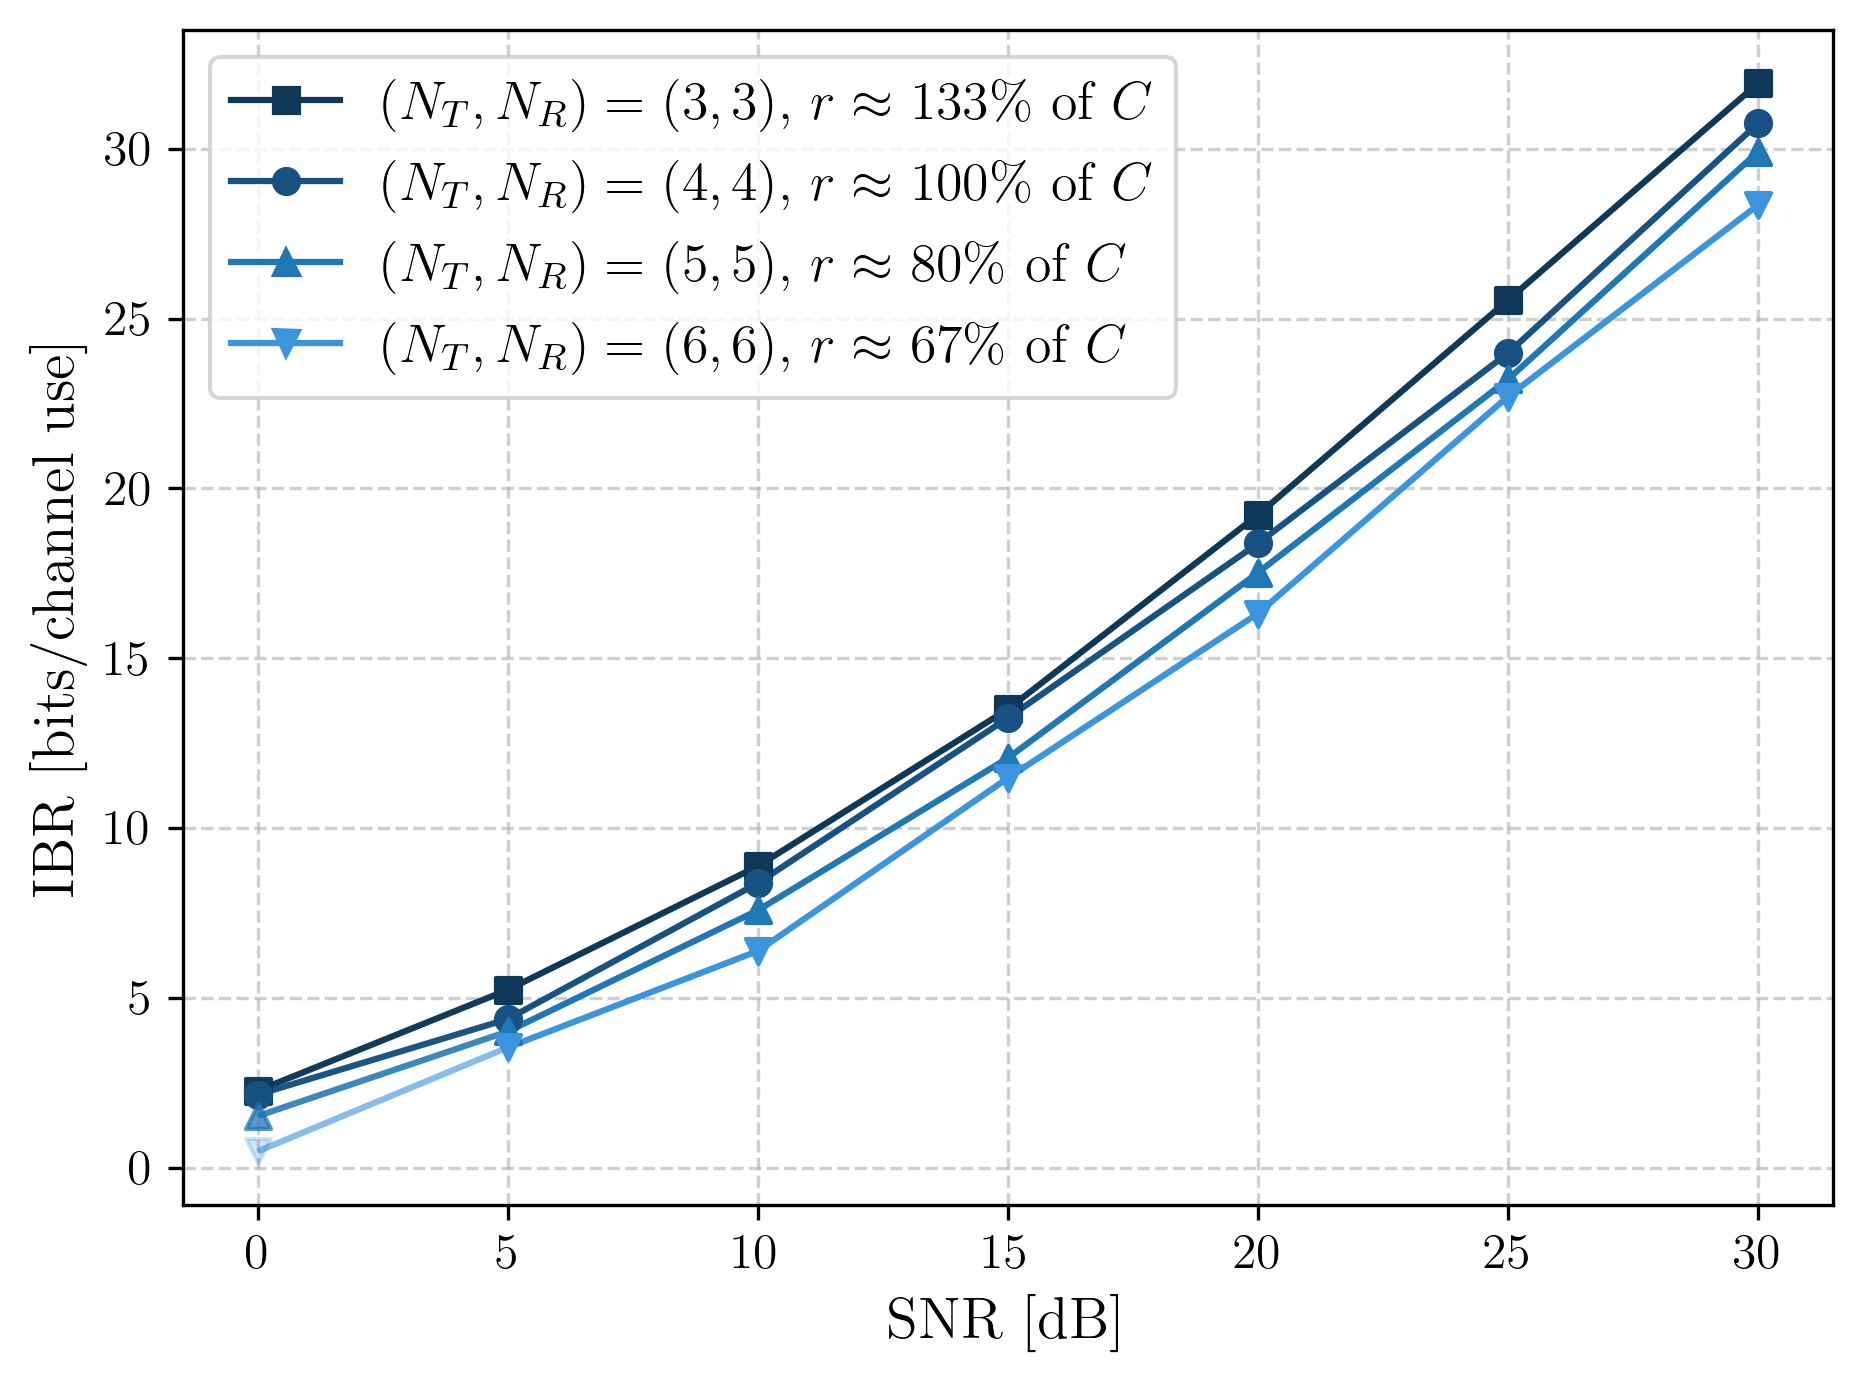
\includegraphics[width=\linewidth]
        {figures/background_material/03_su_mimo_precoding/impact_antennas/variable_ber_ibr_vs_snr.png}
        \caption{}
        \label{subfig:impact_antennas_variable_ber_4x4_adaptive_ba_ibr_vs_snr}
    \end{subfigure}
    \caption[Impact of the antenna count on the system performance (constant IBR comparison)]
    {Illustration of the impact of the antenna count on the system performance for a system adaptive bit allocation. The (a) \ac{BER} and (b) \ac{IBR} are shown as a function of \ac{SNR}, for five different antenna configurations. The rate factor of each configuration is adjusted so that all systems achieve approximately the same \ac{IBR} at each \ac{SNR}.}
    \label{fig:impact_antennas_variable_ber_4x4_adaptive_ba}
\end{figure}

In summary, equipping both the \ac{TX} and \ac{RX} with more antennas enables either higher throughput or higher reliability, at the cost of increased hardware complexity and computational load.

\subsection{Analytical Validation}
\label{subsection:analytical_results}
% ===============================
%    Analytical Validation
% ===============================

As established in Section~\ref{subsection:optimal_precoder_design}, the \ac{SVD}-based precoder and combiner decouple the \ac{SU}-\ac{MIMO} channel into $R_H$ parallel eigen subchannels, each of which can be treated as an independent \ac{SISO} link.
This decomposition enables an analytical evaluation of the total system \ac{BER}.

Because the number of transmitted bits can differ across eigen subchannels, the total \ac{BER} is computed as a weighted average of the subchannel \acp{BER}, with weights proportional to the corresponding \acp{IBR}:
\begin{equation}
\label{eq:analytical_ber_su_mimo}
    \mathrm{BER} = \frac{1}{\mathrm{IBR}} \sum_{i=1}^{R_H} \mathrm{IBR}_i \, \mathrm{BER}_i.
\end{equation}

The \ac{BER} on each eigen subchannel equals the \ac{BER} of a scalar \ac{AWGN} channel.
For subchannel $i$, the effective signal power is determined by the allocated transmit power scaled by the corresponding subchannel gain, while the noise power remains unchanged.
Although the subchannel gains are random variables~\cite{singular_values_distribution}, they are treated as fixed within each analytical evaluation, and the resulting \ac{BER} is then averaged over multiple channel realizations.
The \ac{BER} of a general scalar \ac{AWGN} channel is derived in Appendix~\ref{appendix:analytical_ber} under the union upper bound and the nearest-neighbour approximation.

Figure~\ref{fig:analytical_validation} compares the analytical expressions with the simulated \ac{BER} curves for a $4 \times 4$ system under adaptive and fixed bit allocation.
In both cases, the nearest-neighbour approximation and the union upper bound closely track the simulation results, which validates the simulation implementation.

\begin{figure}[htb]
    \centering
    \begin{subfigure}[c]{0.495\textwidth}
        \centering
        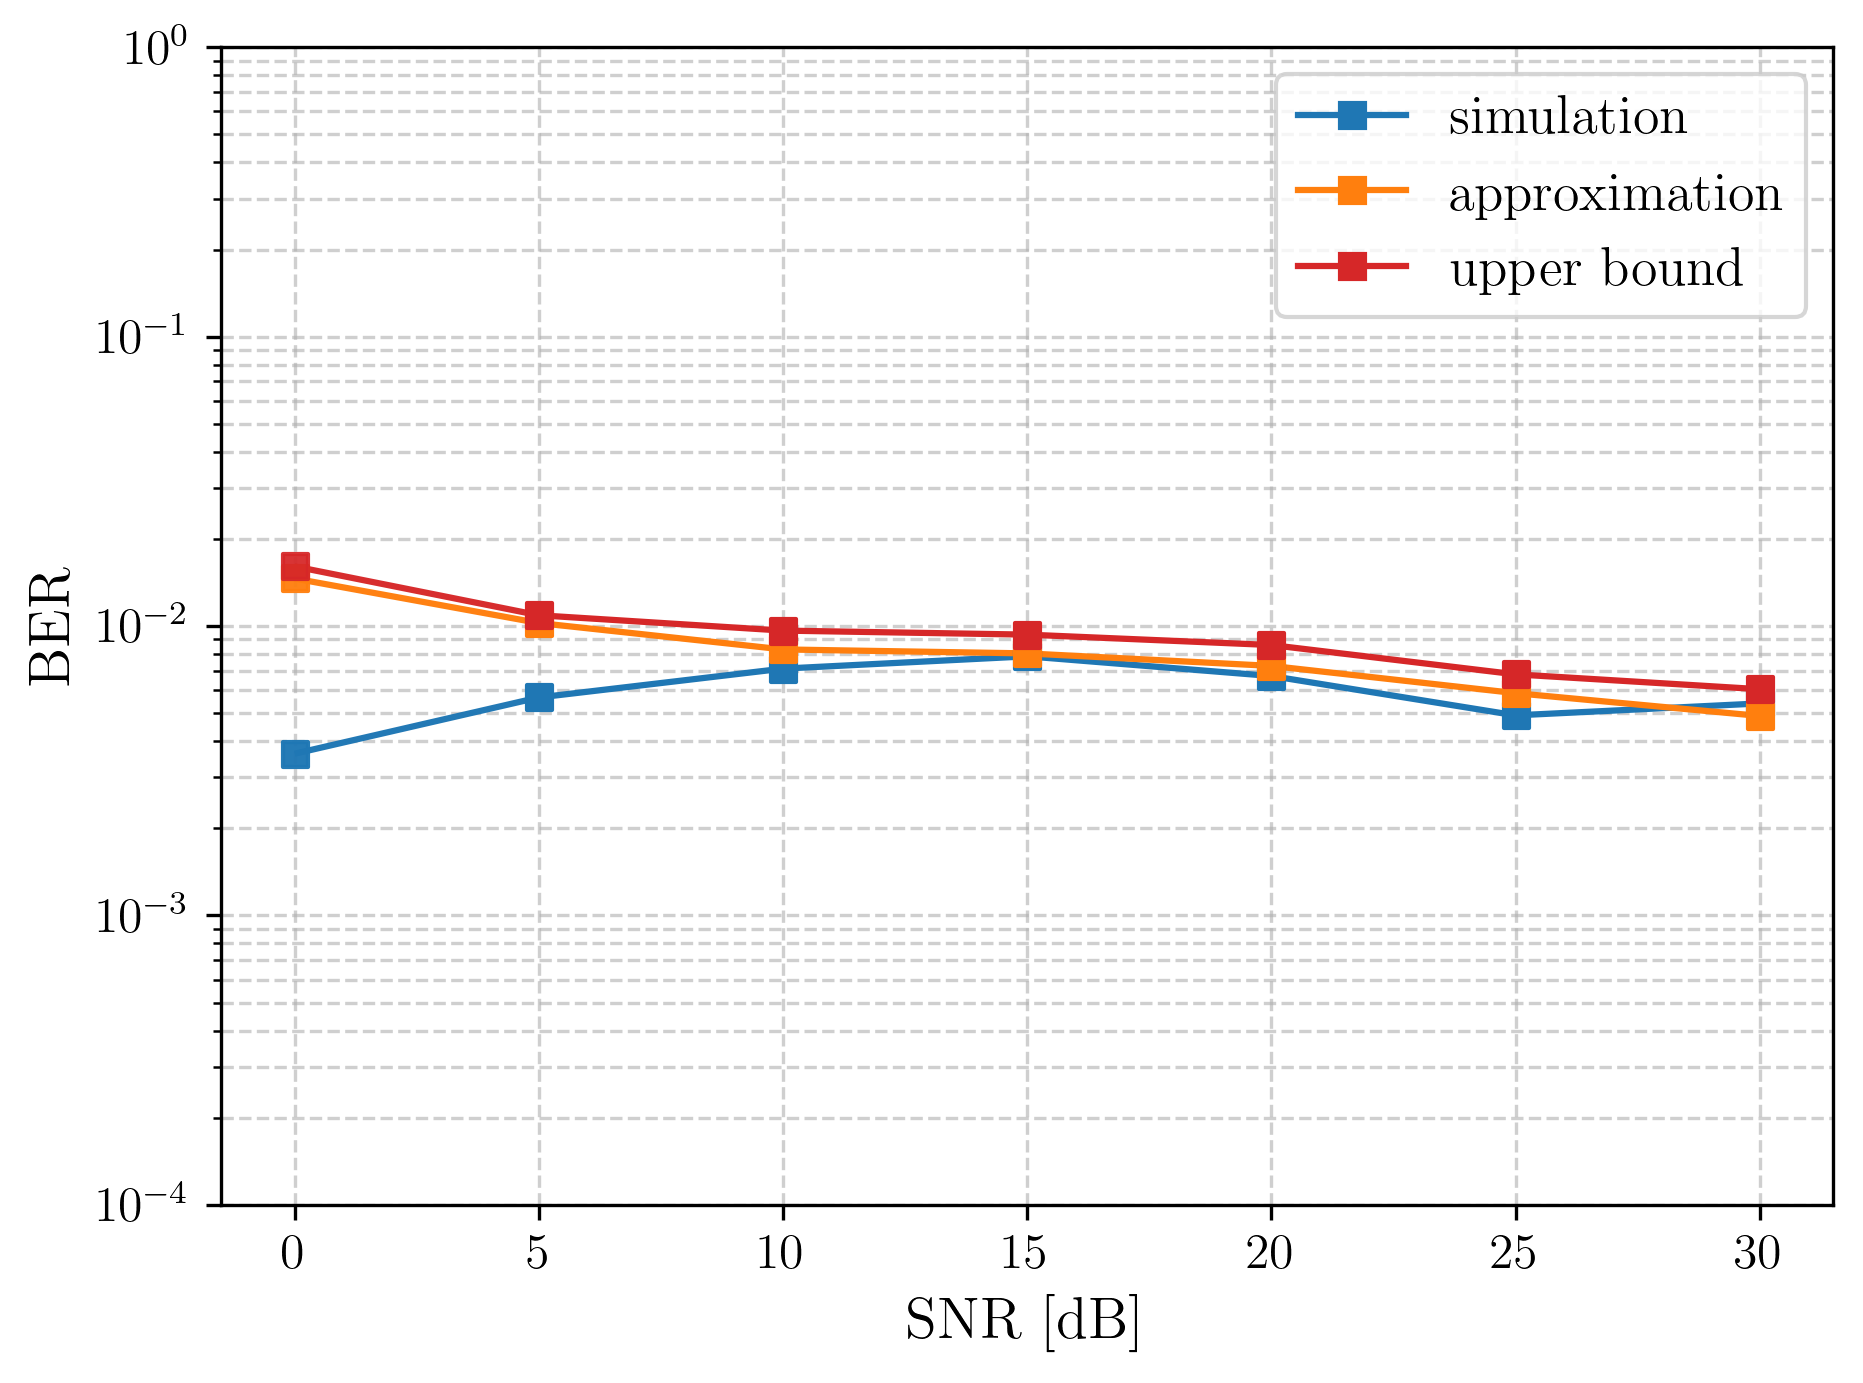
\includegraphics[width=\linewidth]
        {figures/background_material/03_su_mimo_precoding/analytical_validation/adaptive_ba_ber_vs_snr.png}
        \caption{adaptive bit allocation}
        \label{subfig:analytical_validation_adaptive_ba_ber_vs_snr}
    \end{subfigure}
    \hfill
    \begin{subfigure}[c]{0.495\textwidth}
        \centering
        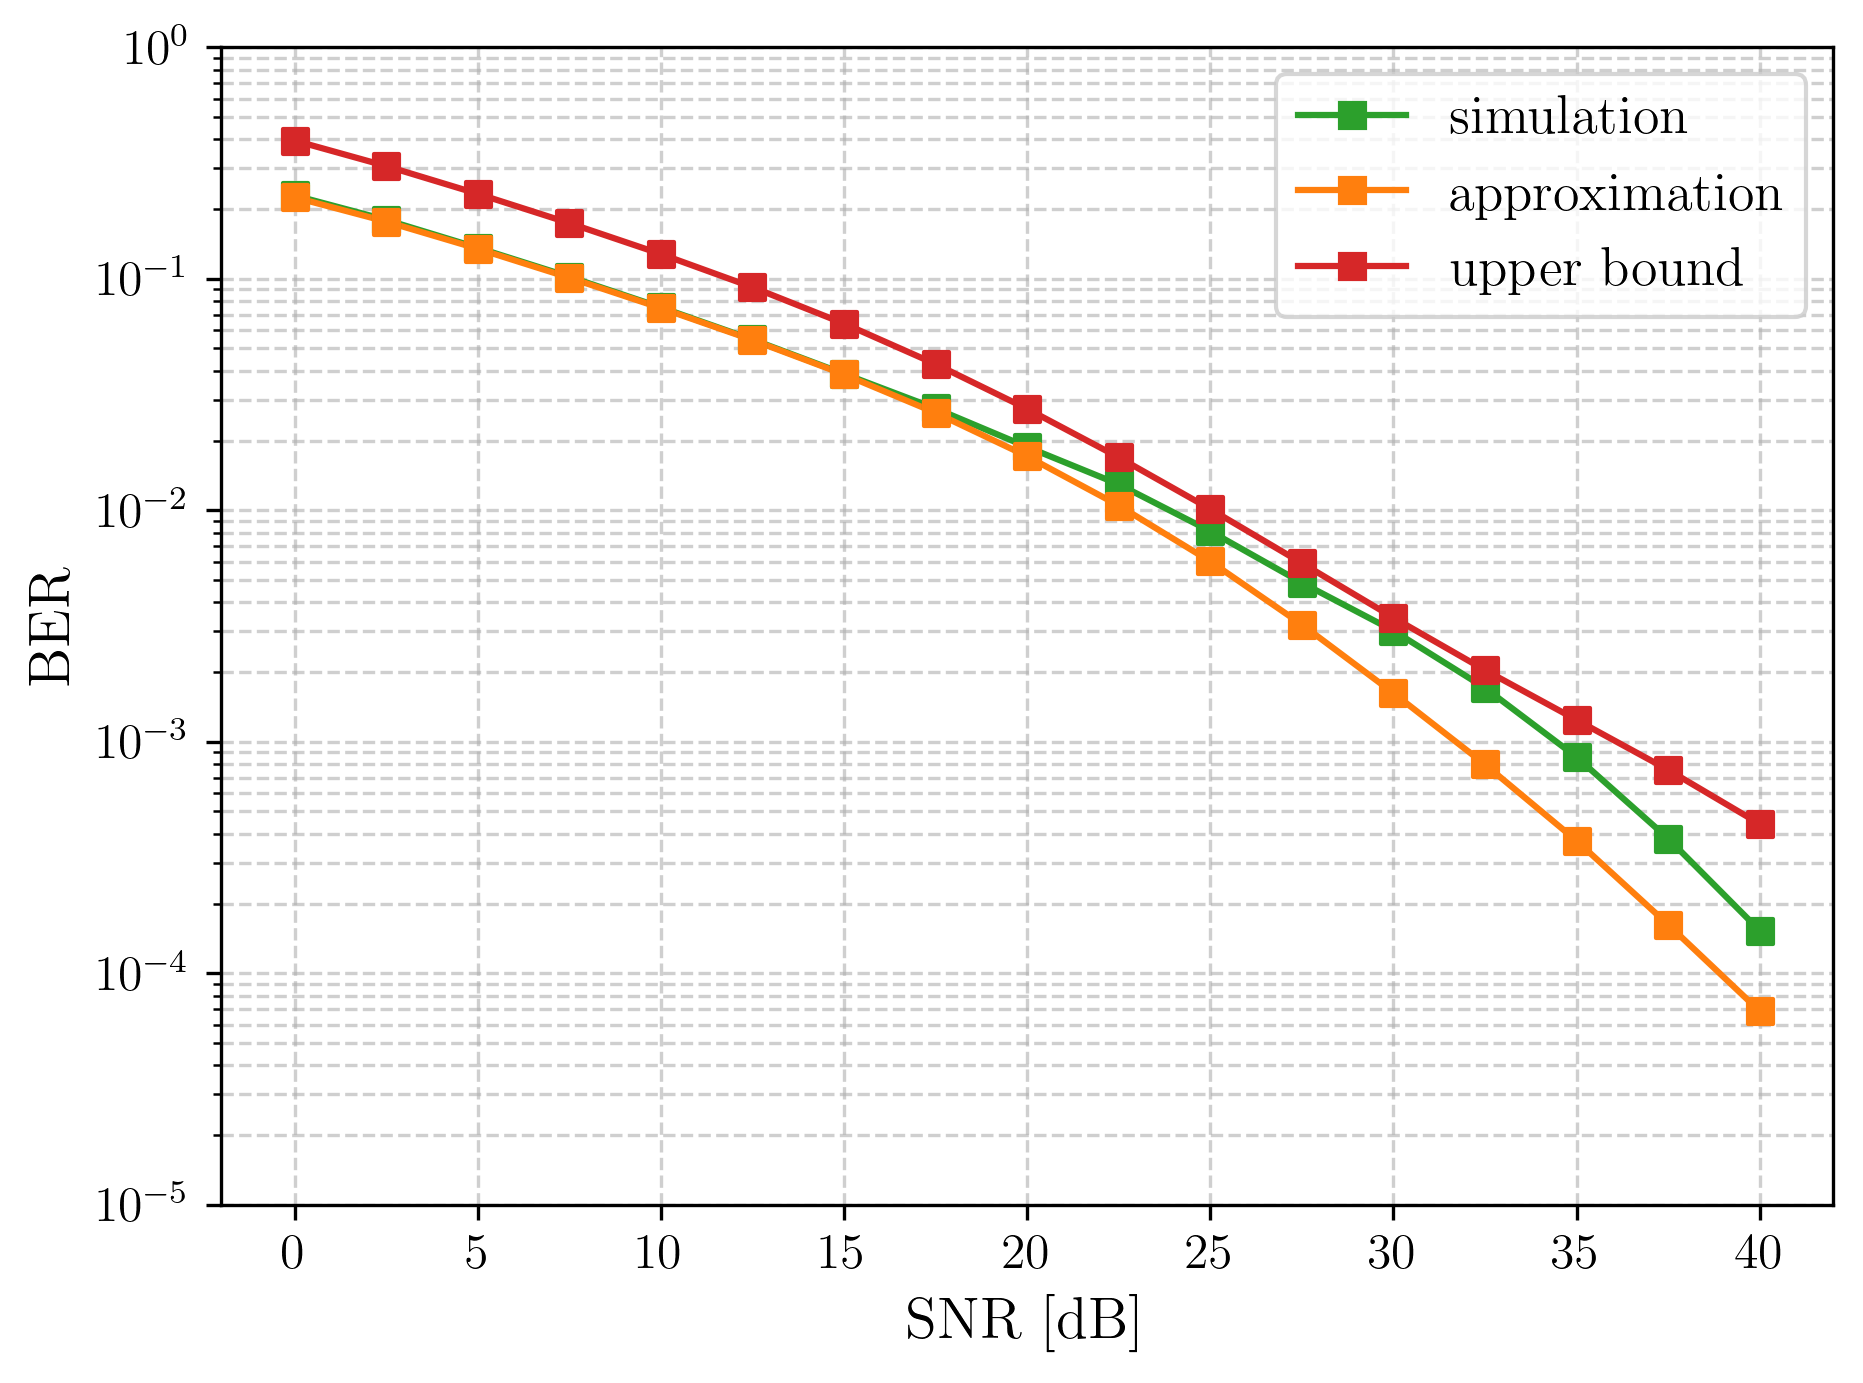
\includegraphics[width=\linewidth]
        {figures/background_material/03_su_mimo_precoding/analytical_validation/4x4_4QAM_fixed_ba_ber_vs_snr.png}
        \caption{fixed bit allocation}
        \label{subfig:analytical_validation_fixed_ba_ber_vs_snr}
    \end{subfigure}
    \caption[Analytical validation of the system performance]
    {Analytical validation of the system performance simulation results for a system with $4$ transmit and $4$ receive antennas. The \ac{BER} is shown as a function of \ac{SNR} for two different bit allocation strategies: (a) adaptive bit allocation with a unit rate factor; and (b) fixed bit allocation, where all subchannels use 4--\ac{QAM} across the entire \ac{SNR} range. In both cases, the simulation results are compared with the union upper bound and nearest neighbour approximation derived in Appendix~\ref{appendix:analytical_ber}.}
    \label{fig:analytical_validation}
\end{figure}
